\chapter{Indirect detection}
\label{chapter:indirect}
\index{Indirect detection}

Indirect Detection (ID) experiments search for the signal illustrated in fig.\fig{DMIDcartoon}:
Dark Matter particles pair-annihilate (or decay) in the galactic halo or outside it, and this results in Standard Model particles that can be detected by looking for an excess in the cosmic ray fluxes measured on Earth (or near it), above the presumed astrophysical contribution. 
This chapter focuses mainly on the `classic' indirect detection signals of
DM particles in the GeV to TeV mass range, typically (but not necessarily) in the WIMP class. 
The same concepts, however,  apply also to lower and higher DM masses, as well as to many different classes of DM candidates. 
We will thus try to keep most of the discussion as broad as possible.

\medskip

The flux of cosmic rays that originates from DM is primarily determined by either the DM annihilation cross section or the DM decay rate. 
An important benchmark for the indirect detection searches is the DM annihilation cross section that leads to the observed cosmological
DM abundance in the case of a thermal freeze-out, see
eq.\eq{sigmavcosmo}.
The size of the expected signal also depends on other aspects of DM: its spatial distribution is particularly important.
The signal rate tends to be higher from regions where DM is expected to be the densest, such as the center of our Galaxy, the inner halo of our Galaxy, nearby galaxies dominated by Dark Matter, the center of the Sun, the center of the Earth...  
However, some of these promising regions (notably the Galactic Center) are also the most complicated ones from the point of view of the underlying astrophysics.
The best detection opportunities might therefore not come from the targets with the highest DM content,
but rather from those with the most favourable signal over background ratio.

The best detection opportunity also depends on the specific cosmic ray species under investigation.
For charged cosmic rays, for instance, it is typically better to focus on antimatter particles (positrons, anti-protons, anti-deuterons\ldots) since they are less likely to be produced in the astrophysical processes 
than the corresponding matter particles.\footnote{See, e.g., ref.~\cite{galCRplots} for comparative plots.} 
This explains why DM studies often concentrate on anti-protons rather than on more  abundant protons: in typical DM models both are produced in equal quantities (in the absence of any model specific matter-antimatter violations), but the astrophysical background is smaller for anti-protons. 

This brings us to the important role the astrophysical backgrounds play in indirect detection: 
the general strategy in indirect detection is to search for a `bump' (an excess) in the spectrum of cosmic rays on top of a background that is assumed to be a power-law in the energy of incoming cosmic ray particles. This power law behaviour is motivated by the  basic acceleration mechanisms of charged particles in astrophysical environments. 
In the real cases, however, the situation is often more complicated: one often encounters deviations from the power-law behaviour, spectral breaks, unexpected bump-like contributions from astrophysical sources,... Several examples that we discuss in detail in chapter \ref{chapter:anomalies} illustrate well how the searches work in practice.


\medskip 

\begin{figure}[!t]
\begin{center}
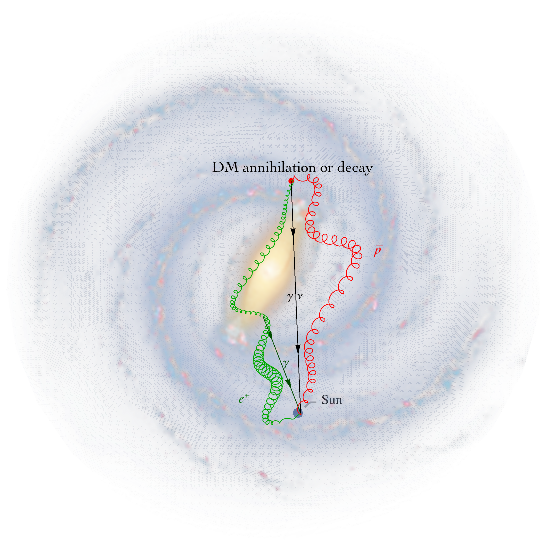
\includegraphics[width=0.47\textwidth]{figs/IndirectDetectionCartoon}\qquad
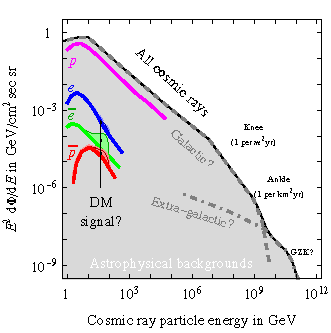
\includegraphics[width=0.42\textwidth]{figs/IndirectDetectionSpectrumCartoonNew}  
\end{center}
\caption[Indirect Detection cartoon]{\em\label{fig:DMIDcartoon} {\bfseries Cartoon of indirect detection}:
DM annihilations or decays in the Milky Way produce SM particles that reach the observer in a solar system,
possibly producing an excess in the energy spectrum of cosmic rays over the observed astrophysical background.}
\end{figure}



In general terms, the particles that are produced by DM annihilations/decays and that we hope to detect are all the stable Standard Model species: photons, neutrinos, positrons, anti-protons, anti-deuterium and maybe even more exotic anti-nuclei such as anti-helium (plus electrons, protons and light nuclei, which are however disfavored by their   more abundant astrophysical backgrounds, as mentioned above).
Each of these messengers possesses distinct advantages and disadvantages, when considered as DM signals:
\begin{itemize}
\item[$\circ$] {\bf High-energy photons ($\gamma$-rays)}  propagate freely in the galactic environment,\footnote{In the extragalactic/cosmological environment, on the other hand, absorption can occur. See section \ref{sec:cosmogammas}.} so that the information about DM lies both in their energy spectrum and in the angular distribution.\footnote{Photon {\em polarization} has also been considered as possible signal of DM  \cite{gammapolarization}. Photons from DM can exhibit a net circular polarization in specific models, such as the decaying asymmetric DM,  DM annihilations that violate P and CP symmetries, DM interactions with ambient cosmic rays, etc. Detecting polarization of high energy photons is, however, very challenging experimentally.} 
However, since DM is electrically neutral it typically produces photons only via subdominant mechanisms, e.g., via loops involving charged particles, or as an ancillary radiation. The photon flux is thus expected to be somewhat suppressed and often model-dependent. 
Since these photons are produced directly in the microphysical processes involving DM, with no interactions with the environment, they are referred to as the {\em prompt $\gamma$-rays}. 

The typically considered sources are very diverse: the area around the galactic center, dwarf galaxies, other nearby galaxies, galaxy clusters or the entire distribution of DM in the Universe (see section \ref{sec:IDgamma}).

\item[$\circ$] {\bf Low-energy photons (X-rays, radio waves)} 
can be produced by the electrons and positrons originating from DM, when these undergo additional interactions (e.g.,\ photons emitted in inverse Compton scattering, synchrotron emission, or bremsstrahlung). 
Such photons constitute a DM signal, but are `doubly indirect', since they depend on the astrophysical
environment that reprocesses the $e^\pm$. Because of this, there are additional uncertainties due to the strength of the magnetic field, the gas density, etc. 
The photons of this type are referred to as the {\em secondary radiation}. 

The low energy photons are, however, not limited to just the secondary production. The $X$-rays and other low energy radiation can also arise directly from the decays of light DM particles with masses in the keV to MeV range, e.g.,\ in models of DM as sterile neutrinos, or in the evaporation of PBH DM.

\item[$\circ$] {\bf Positrons} diffuse in the galactic magnetic fields, which randomizes their directions, so that they do not directly track back to the DM distribution. The information about DM therefore lies only in the energy spectrum. 
However, the latter is significantly affected by the fact that positrons, while propagating through the Galaxy, lose energy through various mechanisms such as 
synchrotron emission, Coulomb scattering, ionization, bremsstrahlung and Inverse Compton (IC) scattering processes. Furthermore, below a few GeV the solar activity distorts their spectrum, and below $\sim$1 GeV it deflects them away, so that they cannot even penetrate into the solar system. 
High-energy positrons coming from the nearby regions of the Galaxy are less affected by diffusion and losses, offering in principle a cleaner access to potential DM contributions to the flux. 


\item[$\circ$] {\bf Electrons}. Similar comments as for positrons apply also to the DM produced electrons,  with the disadvantage of a higher astrophysical background. The advantage, on the other hand, is that at high energies  it is easier to measure the total $e^- + e^+$ flux rather than the positron flux alone.

\item[$\circ$] {\bf Anti-protons} diffuse in the galactic magnetic fields, which randomizes their directions.
Unlike $e^\pm$, they undergo negligible energy losses, up to some scatterings on matter in the galactic plane.
This means that even far-away regions of the Galaxy contribute to the anti-proton flux  measured on Earth, and therefore
its magnitude 
has significant astrophysical uncertainties.
Because of the limited energy losses, the spectral shape is somewhat preserved and thus the information about DM lies also in it. However, compared to $e^\pm$ case, the anti-proton spectra for different DM annihilation/decay channels are more self-similar and thus carry less discriminating power (see section \ref{DMspectra}).
The solar activity again distorts the spectrum below a few GeV and deflects anti-protons away from the solar system for energies below a fraction of a GeV.

\item[$\circ$] {\bf Anti-deuterons}. Nuclei of anti-deuterium can be synthesised via the coalescence of an anti-proton and an anti-neutron produced in the DM annihilation or decay process. The expected yield is very small. On the other hand, the astrophysical background is also expected to be small and, notably, is expected to peak in a range of energies different from the one typical of a  DM signal, thanks to the differing kinematics of the two production mechanisms. The propagation of anti-deuterons in the galactic environment is analogous to anti-protons. Heavier anti-nuclei, such as anti-helium, can be produced in a completely analogous way, with the important penalty of a much more suppressed flux, due to the need for more anti-nucleons to coalesce.

\item[$\circ$] {\bf Neutrinos} propagate freely in the Galaxy and can also propagate through the dense matter of the Earth and of the Sun,
up to multi-TeV energies.
The small interaction cross sections make the detection of neutrinos more difficult than, e.g., of gamma rays. Furthermore, the neutrino energy can often be reconstructed only partially because they are measured indirectly via the detection of charged particles (e.g.\ up-going muons) produced by a neutrino interacting in the material of a neutrino telescope, or in the rock or water or ice surrounding it. 
On the other hand, the  neutrino interaction cross section increases with energy, thus partly compensating the decrease in flux for larger DM masses.
Possible sources of neutrinos from DM are the same as those for photons, but in addition, also the center of the Sun and, less promising, the Earth.
 
\end{itemize}

Pioneering works have proposed these different messengers as a promising avenue for DM discovery already starting in the late-1970's~\cite{PioneersDMID}. 
Gamma rays from annihilations were first considered in Gunn et al.~(1978), Stecker (1978), and Zeldovich et al.~(1980),\footnote{The specific case of gamma ray lines was first discussed in Srednicki, Theisen and Silk (1986) and in Bergstrom and Snellman (1988), in \cite{sharpfeatures}.} and then revisited in Ellis et al.~(1988). 
Anti-protons were first discussed in Silk \& Srednicki (1984), Stecker et al.~(1985) and then more systematically in Ellis et al.~(1988), Rudaz \& Stecker (1988), Stecker \& Tylka (1989). 
Positrons were discussed in Silk \& Srednicki (1984), Ellis et al.~(1988), Rudaz \& Stecker (1988), Turner \& Wilczek (1990). 
Anti-deuterons have been first discussed in \arxivref{hep-ph/9904481}{Donato et al.~(2000} and \arxivref{0803.2640}{2008}), \arxivref{astro-ph/0510722}{Baer \& Profumo (2005)}, 
\arxivref{0908.1578}{Kadastik et al.~(2010)}.
The similar case of anti-helium was first considered in \arxivref{1401.2461}{Carlson et al.~(2015)} and \arxivref{1401.4017}{Cirelli et al.~(2015)}. 
Radio-waves from synchrotron radiation from DM were first explored in Berezinsky et al.~(1992), Berezinsky et al.~(1994), \arxivref{hep-ph/0002226}{Gondolo (2000)}, \arxivref{astro-ph/0101134}{Bertone et al.~(2001)} and later in \arxivref{astro-ph/0402588}{Aloisio et al.~(2004)}. 
Cosmological gamma rays were first discussed in Gunn et al.~(1978) and Stecker (1978), but then systematically reconsidered in \arxivref{astro-ph/0105048}{Bergstrom et al.~(2001)} and \arxivref{astro-ph/0207125}{Ullio et al.~(2002)}. 
Inverse Compton gamma rays from DM have only been  considered relatively recently as a possible signal 
(see e.g.\ \arxivref{astro-ph/0403528}{Baltz \& Wai (2004)}, \arxivref{0811.3641}{Cholis et al.~(2009)}, \arxivref{0812.0522}{Zhang et al.~(2009)}), 
and similarly for bremsstrahlung gamma rays in \arxivref{1307.7152}{Cirelli et al.~(2013).}  
Neutrinos from the center of the Sun and the Earth were first considered by Gould (1987)~\cite{DMnu}.

\medskip

The first step in computing the indirect detection signals is to calculate the spectra of SM particles as they emerge from DM annihilation or decay, i.e., the spectra at production. These are discussed in section~\ref{DMspectra}, in a model-independent way. 
The spectra at production then have to be convoluted with the information about the source (the  distribution of DM, in the Galaxy or elsewhere, as well as the distributions of gas, light and magnetic fields for the secondary radiation) and on the propagation of the SM particles in the astrophysical environments. These aspects are covered in sections \ref{sec:IDgamma} to \ref{sec:boost}. 
More precisely, in section~\ref{sec:IDgamma} we discuss the basic observables for prompt $\gamma$-rays, and in section~\ref{sec:neutrinosID} for neutrinos. 
In section~\ref{sec:e+e-} we discuss electrons and positrons, including, in particular, their propagation in the Galaxy, while in section~\ref{anti-protons} we discuss anti-proton fluxes and their propagation, and in section~\ref{sec:antideuterons} a similar case of anti-deuterons and anti-helium.
Section~\ref{sec:secondary photons} is dedicated to the computation of fluxes of secondary radiation: inverse Compton $\gamma$-rays, bremsstrahlung $\gamma$-rays and synchrotron radiation. 
Section~\ref{sec:boost} discusses which modifications of the formalism are needed in order to take into account several possible sources of enhancements.


The rest of the chapter can be read in two different ways. On the one hand, after section~\ref{sec:boost} the reader might want to jump directly to section~\ref{sec:IDstatus}, 
where we review the current status of the searches in the field, mostly in terms of constraints on DM annihilations/decays. 
(The existing anomalies and possible signals of detection are  covered in chapter \ref{chapter:anomalies}.) Alternatively, one can continue with sections~\ref{sec:DMnu} to~\ref{sec:BBNconstraints}, which contain a variety of other indirect constraints on DM, before moving to section~\ref{sec:IDstatus}. 
Section~\ref{sec:DMnu} deals with neutrinos from the Sun or the Earth: they require a separate treatment that is distinct from our discussion of galactic cosmic rays, both in terms of spectra at production and in terms of the peculiar propagation in celestial bodies, including oscillations. Section~\ref{sec:DMinstars} discusses DM annihilations/decays that occur inside astrophysical objects.
Section~\ref{sec:cosmoconstraints} describes the impact of
DM annihilations/decays during the so-called dark ages of cosmology, i.e.,~on the CMB and on reionization.
Section~\ref{sec:BBNconstraints} gives constraints on DM due to Big Bang Nucleosynthesis.
Finally, section~\ref{sec:UDM:indirect} reviews astrophysical searches for ultralight DM. 

\smallskip

While, as already mentioned above, this chapter is mostly oriented toward the indirect detection of GeV to TeV particle DM~\footnote{For this range of masses, most of the tools and the results in this chapter can be reproduced with the {\tt PPPC4DMID}~\cite{PPPC4DMID}.}, most of the discussion of the underlying physics remains  relevant also for other ID signals, e.g., sub-GeV particle DM (its status is discussed in section~\ref{sec:IDconstraints}), cosmic rays from evaporating Primordial Black Holes (see section~\ref{sec:PBHs}), or $X$-rays from decaying sterile neutrino DM (see e.g.~section~\ref{sec:3.5keV}).



\section{Energy spectra at production}\index{Indirect detection!energy spectra}
\label{DMspectra}

\begin{figure}[!t]
\begin{center}
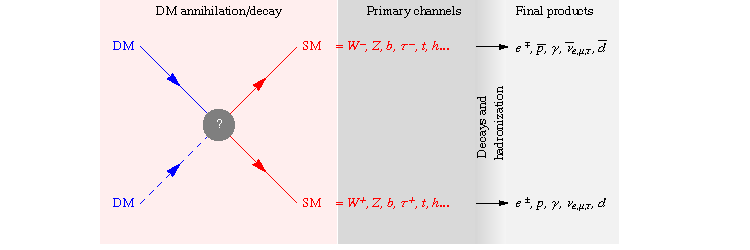
\includegraphics[width=0.9\textwidth]{figs/IDscheme} 
\end{center}
\caption[Indirect Detection scheme]{\em\label{fig:IDscheme} {\bfseries DM Indirect Detection}: the general schematic, illustrating the generation of primary particle spectra.}
\end{figure}


DM particles pair-annihilate (or decay) in astrophysical environments, thereby creating SM particles that then undergo the processes of decay, showering and hadronization. The end result are fluxes of stable SM particles  ($e^\pm,\bar p, \bar d, \gamma,  
\nubarnu_{e,\mu,\tau}$) that can be searched for in cosmic rays as a signal of DM. The whole process is succinctly represented in fig.~\ref{fig:IDscheme}.

\medskip

For many phenomenological analyses, it is useful to compute such fluxes in a model independent way: in the first step one assumes that the DM annihilations or decays produce a SM final state that is a particle--antiparticle pair (e.g.,~$W^+W^-$, $b \bar b$, $\mu^+\mu^-$,\ldots). These are referred to as the {\em primary (annihilation/decay) channels}. For each primary channel one can then calculate the spectra of stable SM particles derived after all the intermediate unstable particles are decayed. 
In any specific DM model the total spectrum is then simply given by a linear sum of contributions from the
 individual primary channels, weighted by the corresponding branching ratios (BRs), dictated by the DM model,
\beq
\frac{dN_{\mbox{\tiny SM}}}{dE} = \left\{
\begin{array}{ll}
\displaystyle  
 \sum_{\rm prim} \frac{\langle  \sigma v\rangle_{\rm prim}}{\langle  \sigma v\rangle_{\rm tot}} \frac{dN_{\mbox{\tiny SM}}^{\rm prim}}{dE} \equiv 
 \sum_{\rm prim} {\rm BR}_{\rm prim} \frac{dN_{\mbox{\tiny SM}}^{\rm prim}}{dE} & {\rm (DM~annihilation),} \\[3mm]
\displaystyle  
\sum_{\rm prim} \frac{\Gamma_{\rm prim}}{\Gamma_{\rm tot}} \frac{dN_{\mbox{\tiny SM}}^{\rm prim}}{dE} \equiv 
\sum_{\rm prim} {\rm BR}_{\rm prim} \frac{dN_{\mbox{\tiny SM}}^{\rm prim}}{dE} & {\rm (DM~decay).}
\end{array}
\right
.
\label{eq:primaryflux}
\eeq
Here $dN_{\mbox{\tiny SM}}^{\rm prim}/{dE}$ is the energy spectrum of cosmic rays produced for a single annihilation into a particular primary channel
(here, $^{\rm prim}$ denotes the primary channel and {\tiny SM} refers to any of the stable cosmic ray SM particles). For instance, $dN_\gamma^W/dE$ is the spectrum of photons produced in a single DM DM $\to W^+W^-$  annihilation. 
The branching ratios are explicitly defined in terms of $\langle  \sigma v\rangle_{\rm prim}$ and $\Gamma_{\rm prim}$, the thermally averaged annihilation cross section and the decay rate for the selected primary channel, while $\langle  \sigma v\rangle_{\rm tot}$ and $\Gamma_{\rm tot}$ denote the corresponding total quantities.
Note that, since DM is cold, the DM annihilation (decay) can be assumed to occur essentially at rest. Each of the two primary particles therefore has the total energy equal to the mass of the DM particle (half of the DM mass). 

In the remainder of this section we work within the above model-independent framework, assuming dominance of two body final states. This does leave aside the possibilities of 3-body or $n$-body annihilations/decays, the annihilations/decays via intermediate states, as well as the annihilations/decays which do not produce a particle-antiparticle pair but rather a combination of different particles in the final state (e.g., the DM$\to W^\pm \tau^\mp$ decay, relevant for gravitinos), etc.\footnote{We will consider some peculiar model-dependent spectra of gamma rays in section~\ref{sec:modeldepgammas}.}  
In some of these cases, the fluxes can be computed by properly combining the model independent building blocks discussed above. In general, however, a dedicated computation has to be performed.

The exhaustive list of primary channels in the model independent approach consists of:
\beq 
\begin{array}{ll}
e^+e^-,\ 
\mu^+\mu^-,\ 
\tau^+\tau^-,\ 
\nu_e \bar\nu_e, \ 
\nu_\mu \bar\nu_\mu, \ 
\nu_\tau \bar\nu_\tau, \\[3mm]
q \bar q, \ 
c \bar c, \ 
b \bar b, \  
t \bar t, \ 
\gamma \gamma,\ 
g g,  \\[3mm]
W^+ W^-,\ 
ZZ,\ 
 hh, \\[3mm]
\end{array}
\label{eq:primarychannels}
\eeq
where  $q ={u,d,s}$ denotes a light quark\footnote{The light quarks are treated collectively since they lead to very similar spectra, at least for $M \gtrsim$ few GeV.} and $h$ is the Standard Model Higgs boson. Some channels (such as $\gamma \gamma$, $\nu\bar\nu$, $gg$) are `unusual' as they are often suppressed in many models (in particular, since DM is neutral, its $\gamma\gamma$ yield is generically expected to be suppressed and as a consequence the 3-body and higher-order effects mentioned above can become relevant), however, from a model-independent point of view they are as viable as any other.



The primary particles' decays, showerings and hadronizations are dictated by the SM physics.  In most studies the predictions for this part are obtained using one of the Monte Carlo simulation programs designed for collider physics \cite{MonteCarlosforDM,PPPC4DMID,CosmiXs}, appropriately modified to take into account the fact that particles that are considered stable on collider scales (such as muons or neutrons) have enough time to decay in the cosmological environments.\footnote{
In Monte Carlo generators the $s$-wave non-relativistic DM DM annihilation is modeled using the equivalent process: the decay of 
 resonance $X$ that has twice the DM mass, $M_{X} = 2M$, 
 and decays into the appropriate pair of Standard Model particles.
 }
{\tt Pythia} is often the default choice, and is also at the base of the results presented here. {\tt Herwig} has also been employed in the literature, while {\tt Geant4} has been used for the specific case of annihilations/decays happening in the dense matter of the Sun, as we will discuss in section~\ref{sec:DMnu}.
The algorithms implemented in {\tt Herwig}, {\tt Pythia}, and other codes, differ both in the treatment of parton showers as well as hadronization. The difference in the predictions due to a choice of the numerical tool thus gives us some estimate of theoretical uncertainties. In most cases these are of the order of 20\%~\cite{PPPC4DMID,MonteCarlosforDM},
although larger discrepancies can appear in some specific cases. 
It is also important to remember that the above tools 
have been designed and tuned for the energies typical in collider physics (GeV-TeV). Extrapolations to lower or higher energies (i.e.,~lighter or heavier DM) in general
reduce the reliability of the results. Recently, there were thus several dedicated efforts  aimed at extending the predictions for spectra in the directions of light and heavy DM~\cite{codeslowEhighE}. 

\begin{figure}[!t]
\begin{center}
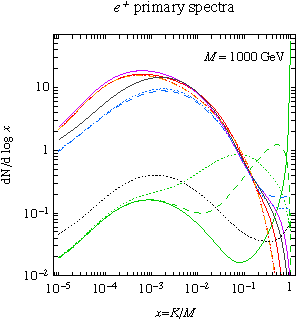
\includegraphics[width=0.26 \textwidth]{figs/spectraproduction_positrons}  ~
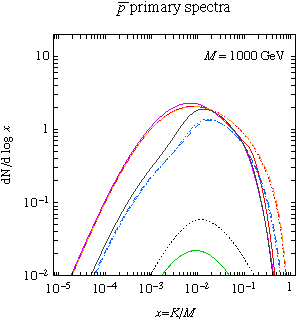
\includegraphics[width=0.26 \textwidth]{figs/spectraproduction_pbar}  ~
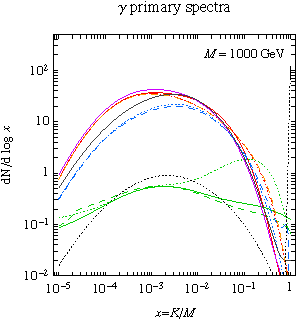
\includegraphics[width=0.26 \textwidth]{figs/spectraproduction_gamma}  ~
\raisebox{0.02\textwidth}{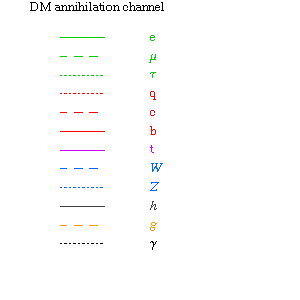
\includegraphics[width=0.15 \textwidth]{figs/spectraproduction_legenda}}
\end{center}
\caption[Indirect Detection spectra at production]{\em\label{fig:spectraatproduction} Examples of {\bfseries primary cosmic ray spectra} from DM annihilations, for DM with a mass of $1 \TeV$, and for different primary channels. The spectra are expressed as a function of $x=K/M$, where $K$ is the kinetic energy of the indicated final state particle.}
\end{figure}

\smallskip

The end product of simulations are the DM produced fluxes of energetic cosmic rays $e^\pm,\bar p, \bar d, \gamma, \nubarnu_{e,\mu,\tau}$. Selected examples of these {\em primary cosmic ray spectra} are illustrated in fig.~\ref{fig:spectraatproduction}. The spectra vary significantly between different primary channels (different SM particles first produced in the DM annihilation/decay). However, they all exhibit a `bump-like' shape, marked by a high-energy cutoff at the DM particle mass and a gently diminishing tail at lower energies, potentially accompanied by additional humps.


It is instructive to examine qualitatively a few cases, and reconstruct the origins of different features appearing in the spectra. Let us start with the DM DM $\to W^+W^-$ annihilations and the induced $e^+$ spectra (dashed blue line in the left panel in fig.~\ref{fig:spectraatproduction}). The  $W$'s can decay leptonicaly ($W^\pm \to \ell^\pm \nubarnu_{\ell}$) or hadronicaly ($W^\pm \to q \bar q^\prime$). The leptonic $W^\pm \to e^\pm \nubarnu_{e}$ decays directly produce the high-energy electrons or positrons that can, for appropriate kinematical configurations, carry almost all of the energy released in the process. This corresponds to the `wedge'  in the spectrum at $x \sim 1$, visible in the dashed blue line. A similar feature is present for the spectra of neutrinos (not shown in the figure). The leptonic $W^\pm$ decays into muons and taus produce, upon further decay of these heavy leptons, more $e^\pm$: since in these cases a significant part of the energy is carried away by the neutrinos, the resulting $e^\pm$ will contribute to the $x<1$ part of the spectrum. The hadronic $W^\pm$ decays produce energetic quarks: they, in turn, decay, fragment and hadronize, producing a host of low energy particles that ultimately decay generating low energy $e^\pm$. They contribute to the prominent hump in the spectra at $x \ll 1$. 

In the $\gamma$-ray spectra (right panel in fig.~\ref{fig:spectraatproduction}), one sees another wedge at $x \sim 1$ for the $W$ primary channel. This corresponds to hard photons radiated by the charged $W^\pm$ (this feature is not present for the $Z$ primary channel). The prominent bump at $x \ll 1$ corresponds to all the photons produced in the subsequent cascades, notably the decays of light mesons created during hadronization (e.g.,~$\pi^0 \to \gamma \gamma$). 



As another example, let us consider the case of DM DM $\to e^+e^-$ annihilations (solid green line in the left panel in fig.~\ref{fig:spectraatproduction}). In the $e^+$ spectrum we can easily recognize the expected $x=1$ spike, smeared towards lower $x$ by final state radiation. The wide bump around $x\sim 10^{-3}$ might be surprising at first sight: it is due to electroweak emissions (discussed in section \ref{sec:EWemissions} below). 

The $\bar p$ spectra (middle panel in fig.~\ref{fig:spectraatproduction}) exhibit a more self-similar shape, largely independent from the primary channel. Anti-protons are produced at the end of the hadronization process, which `washes away' the peculiarities related to the initial particles, where only the purely leptonic primary channels are distinct from the rest. 
The small production of $\bar p$ from the purely leptonic $e^+e^-$ and $\mu+\mu^-$ channels is due to electroweak emissions, while $\tau^+\tau^-$ also has hadronic decay modes.

Similar considerations allow to understand many of the qualitative features of the other spectra as well. 

\subsection{Production of light nuclei} \index{Indirect detection!light nuclei}
\label{DMspectraDbarHe}
Antideuterons (and antihelium nuclei) deserve a separate discussion~\cite{antiD}. Antideuterons can be produced via the fusion of a $\bar p  \bar n$ pair, a process usually described by a simple `coalescence model'. The idea behind this approach is very simple: the anti-nucleons produced in the DM annihilation/decay process can merge to form an anti-nucleus, if the difference in their momenta is less than a certain threshold, the effective quantity called the coalescence momentum $p_{\rm coal}$. The value of $p_{\rm coal}$ is a free parameter of the model that has to be determined from a comparison with the experimental data, for instance from the $e^+e^- \to \bar d X$ collider reactions (here, $\bar d$ denotes an anti-deuteron, and $X$ inclusively any other  final state). The na\"ive estimate $p_{\rm coal} \approx \sqrt{m_N \, B_d} \approx 46$ MeV, with $m_N$ the nucleon mass 
and $B_d = 2.2$ MeV  the deuteron binding energy, is not too far from the typically adopted values for $p_{\rm coal}$, which range from 66 to 226 MeV.

One way of implementing the above prescription is to take the Monte-Carlo-produced spectra of $\bar p$ and $\bar n$ discussed above (they are typically equal, barring unusual isospin violation) and combine them using the coalescence prescription. One can show that the resulting $\bar{d}$ spectrum then reads
\begin{equation}
 \frac{dN_{\bar{d}}}{dT_{\bar{d}}}=\frac{4\pi}{3}p_{\rm coal}^{3}\frac{m_{\bar{d}}}{m_{\bar{n}}m_{\bar{p}}}\frac{1}{\sqrt{T_{\bar{d}}^{2}+2m_{\bar{d}}T_{\bar{d}}}}\left(\frac{dN_{\bar{p}}}{dT_{\bar{p}}}\right)_{T_{\bar{p}}=\sfrac{T_{\bar{d}}}{2}}
 \left(\frac{dN_{\bar{n}}}{dT_{\bar{n}}}\right)_{T_{\bar{n}}=\sfrac{T_{\bar{d}}}{2}},
 \label{eq:antiD}
\end{equation}
where $T$ denotes the kinetic energy. This formula shows 
that the $\bar d$ yield depends significantly on the value of $p_{\rm coal}$. The $\bar d$ spectrum is also  `doubly suppressed' with respect to the already small $\bar p$ and $\bar n$ spectra: as a rule of thumb, the $\bar d$ yield is found to be a factor of ${\cal O}(10^{-5})$ smaller than the $\bar p$ one.

The above procedure assumes, however, that the events are spherically symmetric, i.e.,~an isotropic emission of the anti-nucleons from the DM annihilation/decay process. This assumption is violated in processes in which the anti-nucleons are produced from boosted initial particles. For instance, for DM DM $\to W^+W^-$ and for a large DM mass, the anti-nucleons are produced in the boosted back-to-back jets produced by the $W^\pm$, enhancing the probability of having  $\bar p \bar n$ pairs with small momentum difference. In order to have the correct prediction for the $\bar d$ yields, the details of the angular distribution of the anti-nucleons in the final state, together with possible (anti-)correlations between them, must be taken into account. 
This has to be done by computing the $\bar d$ spectrum numerically, enforcing the coalescence prescription on an event-by-event basis in the Monte Carlo itself. This feature is included in {\tt Pythia} since v8.240.

Identical considerations apply to the anti-helium production \cite{Antihelium}, in its two possible isotopic forms, $^3\overbar{\rm He}$ and $^4\overbar{\rm He}$. 
Each additional coalescing anti-nucleon brings an additional factor of $dN/dT$, while in the naive formula in eq.~(\ref{eq:antiD}) the $p_{\rm coal}^3$ factor is replaced by $p_{\rm coal}^{3(A-1)}$, where $A$ is the mass number. The final yield can be expected to be suppressed by an additional factor of ${\cal O}(10^{-5})$ per added anti-nucleon: in practice, only $^3\overbar{\rm He}$ may be produced in non-negligible amounts. 
Its coalescence can proceed from either a $\bar p \bar p \bar n$ or a $\bar p \bar n \bar n$ triplet. In the former case the $^3\overbar{\rm He}$ is formed directly, but the efficiency is suppressed by Coulombian repulsion between the two anti-protons. In the latter case, $^3\overbar{\rm He}$ is the result of the formation of an anti-tritium that subsequently decays into a $\overbar{\rm He}$ in a process that, given the typical propagation scales, can be considered to be instantaneous. 
In the simulations, the coalescence prescription needs to be generalized appropriately: one can require that all the three differences among the anti-nucleon momenta in the rest frame of the center of mass are smaller than $p_{\rm coal}$, or that the three momenta lie inside a minimum bounding sphere in momentum space with a diameter determined by $p_{\rm coal}$. 
In practice, the differences in the yields obtained using different prescriptions are small, compared to other uncertainties. 

The value of $p_{\rm coal}$ is hard to establish, given the scarcity of the $\overbar{\rm He}$ collider data. One option is to determine it from the $p_{\rm coal}$ value for $\bar d$  by scaling it with the binding energy as $p_{\rm coal}^{\rm He} \approx \sqrt{B_{\rm He}/B_{d}} \ p_{\rm coal}^{d}$. The  values typically adopted in the literature therefore span  a large range $p_{\rm coal}^{\rm He} \approx 200-400\,{\rm MeV}$. 
More sophisticated methods than the coalescence prescription have also been put forward and employed in the recent literature. 





\subsection{Electroweak emissions} 
\label{sec:EWemissions}

\begin{figure}[!t]
\begin{center}
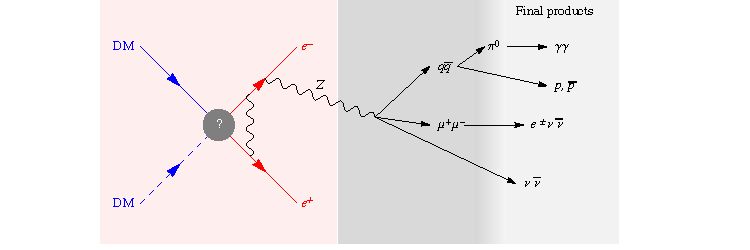
\includegraphics[width=0.85 \textwidth]{figs/IDschemeEWcorr}
\end{center}
\caption[EW corrections scheme]{\em \small \label{fig:EWscheme} {\bfseries Illustration of electroweak corrections}, for the case of a primary annihilation into $e^+e^-$. In the absence of any electroweak emissions, the resulting primary cosmic ray spectrum would 
consist of just the $e^+e^-$ pair, i.e.,~a delta function at $x = K/M =1$ in the $e^\pm$ spectrum. The emission of a weak boson (a $Z$ in this case), as well as the accompanying virtual boson exchange (vertex correction), modify the spectrum. The $Z$ decays, which then gives 
lower energy $e^\pm$, as well as other particle species. 
The hadronic decays of the gauge boson produce quarks that hadronize into, among other things, anti-protons, which can therefore emerge from a purely leptonic DM channel.}
\end{figure}


Among the different processes occurring after the production of primary particles, the electroweak emissions are particularly relevant. 
This term denotes the radiation of  $W$ or $Z$ electroweak gauge bosons from outgoing particles. (The $W$ and $Z$, of course, subsequently decay.)
This emission is a higher order process with respect to the 2-body annihilation/decay and is therefore suppressed by an additional weak coupling. However,
such bremsstrahlung corrections are enhanced by one or more powers of $\ln (M /M_W)$ logarithms, which become large for $M \gg M_W$, compensating the suppression. 
Consequently, the electroweak emissions have only recently been identified as significant for DM indirect detection~\cite{EWbrem}, particularly as interest in TeV DM masses has grown. 
For instance, these effects were absent in {\tt Pythia} versions prior to v8.176 (2013). 
This prompted the authors of \cite{PPPC4DMID} to add them, working at single emission order, including vertex corrections, by `post-processing' the {\tt Pythia} output.
Subsequent {\tt Pythia} versions have gradually incorporated these effects, including higher order corrections.
 Furthermore, these effects have been explicitly addressed in more recent codes~\cite{CosmiXs,codeslowEhighE}, including those developed to study extremely heavy DM.




Phenomenologically, the effects of the electroweak radiation can be particularly relevant for the leptonic and 
$\gamma\gamma$ primary channels. 
The emissions of $W$'s and $Z$'s, and their subsequent decays, lead to additional particles in the final state, and can therefore modify significantly the flux of $\gamma$'s  and $e^\pm$ at lower energies, $E\ll M$. 
Moreover, the $W/Z$ radiation leads to a $\bar p$ contribution, which would have been absent in the leptonic and $\gamma\gamma$ primary channels, were the electroweak corrections to be neglected. This also holds true for the neutrino primary channels, 
where the electroweak emissions result in nonzero $e^\pm$'s, $\gamma$, and $\bar p$ primary ray spectra. 

There are other instances where the electroweak corrections are important. For instance, the annihilation rates of Majorana DM particles into light fermions are helicity suppressed. Inclusion of the electroweak emissions lifts the suppression, and allows the annihilation to proceed in an $s$-wave, implying a much larger cross section and modified spectra. It is also good to keep in mind that the EW emission can occur from the final state particles, from the internal states running in the loop, or even from the  initial DM states, if DM is part of an EW multiplet (its neutral component)~\cite{EWbrem}.



\section{Gamma rays}\index{Indirect detection!$\gamma$}\index{$\gamma$}
\label{sec:IDgamma}

In this section, we examine the calculation of observables related to prompt gamma rays produced in DM annihilations/decays. We defer the discussion of secondary radiation, which can also have energy in the domain of gamma rays, to section  \ref{sec:secondary photons}.

\smallskip

To search for photon signals from DM  there are a number of varied {\em ``best targets''}. Ideally, these are regions with high DM densities or regions with low astrophysical `backgrounds', resulting in a favorable signal-to-noise ratio. The demarcation between the two requirements is not clear cut: environmental factors may render certain regions more suitable than others, despite comparable DM densities and backgrounds.

Typically, the experimental focus is on:
\begin{itemize}
\item[$\circ$] 
{\bf The Milky Way Galactic Center (GC)}, or small regions around or just outside it, often referred to as the Galactic Center Halo (GCH).
\item[$\circ$] 
{\bf Wide regions of the Galactic Halo (GH)},  up to several tens of degrees wide in latitude and longitude, and away from the Galactic plane. The average DM density is lower in these regions than it is close to the GC. However, the astrophysical contribution is also much lower, since this is heavily concentrated in the Galactic plane. The GH regions are also promising for the detection of the secondary radiation, given that the DM-produced CRs have less competition from the  CRs of astrophysical origin than they do in the Galactic plane. 
\item[$\circ$] 
{\bf Globular clusters (GloCs)}, i.e., dense agglomerates of stars with the total mass of order $10^5 \, M_\odot$, 
embedded in the Milky Way galactic halo or in the subhalo of dwarf galaxies.\footnote{The differentiation between a (large) GloC and a (small) dwarf galaxy is nuanced; typically, the former exhibits greater density, an abundance of stars, and proximity to Earth.
} 
The DM content (and its distribution) in GloCs 
is still subject to debate~\cite{DMinGloC}. 
The interest in GloCs stems from four key aspects:
i) they could have originated from a primordial DM sub-halo, possibly retaining some trapped DM;
ii) the density of baryonic matter could generate a DM concentration via attraction, enhancing DM annihilation flux, and even have an effect on the DM halo of the host galaxy;
iii) they are closer than dwarf galaxies and would therefore lead to a brighter DM annihilation flux on Earth; 
iv) they might host an Intermediate Mass Black Hole (IMBH), which could also significantly enhance the DM annihilation flux. 
\item[$\circ$] 
{\bf Subhalos of the GH.} The positions of subhalos are, however, unknown a priori. See the discussion in section~\ref{sec:asphericalcow}.
\item[$\circ$] {\bf Satellite galaxies of the Milky Way,} often of the dwarf spheroidal (dSph) class, such as Sagittarius, Segue 1, Draco, and several others. These satellite galaxies are star deprived and are believed to be DM dominated. See the discussion in section~\ref{sec:dwarfs}.
\item[$\circ$] {\bf Large scale structures in the relatively nearby Universe,} such as the galaxy clusters: 
the Virgo, Coma, Fornax, and Perseus clusters, as well as several others. 
In such larger objects the DM particles have  higher velocities on average, so that these are good probes of DM with velocity-suppressed $p$- or $d-$wave annihilations~\cite{2304.10301}.
\item[$\circ$] {\bf The entire Universe,} by measuring  the {\em cosmological} flux of redshifted $\gamma$-rays at the position of the Earth, and originating from DM annihilations in all the halos along the line of sight, spanning the complete recent history of the Universe. 
This flux is often termed as `extragalactic', though one needs to be careful not to confuse it 
with the flux from specific large structures located outside our galaxy, and mentioned in the previous item. 
Alternatively, it is described as `isotropic' (IGRB, Isotropic Gamma-Ray background), though it is only nearly isotropic (see section \ref{sec:correlations}). 
\end{itemize}
In the rest of this section,  we will discuss the main quantities related to gamma-ray observations from these various targets.

\subsection{$\gamma$ from the Milky Way}\index{Milky Way!indirect detection}\index{$\gamma$!from the Milky Way}
\label{sec:IDgammaMW}
The {\em differential flux of photons} from a given angular direction $d\Omega$, produced by the annihilations of self-conjugated DM particles (e.g.\ Majorana fermions) inside the Milky Way, is given by
\beq 
\label{gammaflux}
\frac{d \Phi_\gamma}{d\Omega\,dE} = \frac{1}{2}\frac{r_\odot}{4\pi} \left(\frac{\rho_\odot}{M }\right)^2  J \, \langle \sigma v\rangle 
\frac{dN_\gamma}{dE}  ,\qquad
J = \int_{\rm l.o.s.} \frac{ds}{r_\odot} \left(\frac{\rho(r(s,\theta))}{\rho_\odot}\right)^2 \qquad {\rm (DM~annihilation)},
\eeq
while for a decaying DM we have, similarly, 
\beq 
\label{gammafluxdec}
\frac{d \Phi_\gamma}{d\Omega\,dE} = \frac{r_\odot}{4\pi} \frac{\rho_\odot}{M } D \, \Gamma
\frac{dN_\gamma}{dE}  ,\qquad
D = \int_{\rm l.o.s.} \frac{ds}{r_\odot} \frac{\rho(r(s,\theta))}{\rho_\odot}  \qquad {\rm (DM~decay).}
\eeq
The radial coordinate $r$, measured from the GC, is given by $r(s,\theta)=(r_\odot^2+s^2-2\,r_\odot\,s\cos\theta)^{1/2}$, while $\theta$ is the aperture angle between the direction of the line of sight (l.o.s., parametrized by variable $s$) and the axis linking the Earth to the GC.
The total energy spectrum of photons produced by DM annihilations/decays, denoted as $dN_\gamma/dE$, is computed in eq.~(\ref{eq:primaryflux}).
If DM is not composed of self-conjugate particles (e.g., if DM particle is a Dirac fermion), then $\sigma v$ in eq. \eqref{gammaflux} must be averaged over DM particles and antiparticles. 
In practice this means that the expression in eq. \eqref{gammaflux} has to be divided by an additional factor of 2, if only particle-antiparticle annihilations are present.
It is also important to note that the above formalism, especially the simple definition of the $J$ factor determined solely by the DM density profile, holds true only when the annihilation cross section is
position independent. If this is not the case, the annihilation cross section must be included as part of the integrand inside the l.o.s.~integral. In particular, if the annihilation cross section is velocity-dependent, which, for instance, happens for $p$-wave or Sommerfeld enhanced annihilations, the calculation of the total flux must include the full DM velocity distribution (see e.g.~\arxivref{2110.09653}{Boucher et al.~(2022)}~\cite{Boucher:2021mii}).

\begin{figure}[!t]
\begin{center}
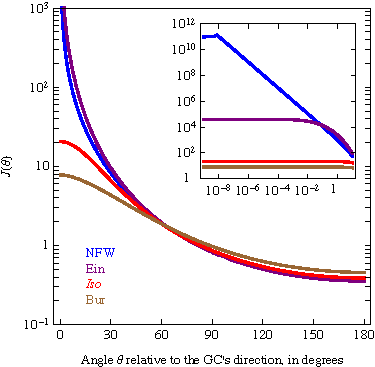
\includegraphics[width=0.48 \textwidth]{figs/Jthetaann} \quad 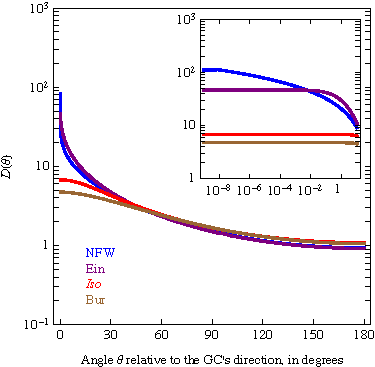
\includegraphics[width=0.48 \textwidth]{figs/Jthetadec}
\end{center}
\caption[Line-of-sight integral $J(\theta)$ and $D(\theta)$]{\em \small \label{fig:Jtheta} $\boldsymbol{J(\theta)}$ {\bfseries for annihilating} (left) {\bfseries and} $\boldsymbol{D(\theta)}$ {\bfseries for decaying} (right) {\bfseries Dark Matter}, for different DM profiles introduced in section \ref{sec:DMdistribution}, with the color coding given in the legend (from bottom to top in the inset: Burkert, Isothermal, Einasto, NFW).}
\end{figure}


\index{J factor@$J$ annihilation factor}\index{D factor@$D$ decay factor}
The  ${\mb J}$ {\bf factor} in eq.~(\ref{gammaflux}) and the ${\mb D}$ {\bf factor}  in eq.~(\ref{gammafluxdec}) include appropriate factors of $r_\odot$ and $\rho_\odot$ (the Sun--GC distance and the DM density at the location of the Sun, see section~\ref{sec:MilkyWay}) to make them dimensionless.\footnote{Alternatively, sometimes two analogous factors are defined, the DM annihilation factor ${\mathcal J} = \int_{\rm l.o.s.} \rho^2(r) = r_\odot \rho_\odot^2\, J$, having units of GeV$^2$/cm$^5$, and the DM decay factor ${\mathcal D} = \int_{\rm l.o.s.} \rho(r) = r_\odot \rho_\odot \, D$, having units of GeV/cm$^2$.} We work in the limit of a spherically symmetric DM halo, so that $J (\theta)$ and $D (\theta)$
 are invariant under rotations around the Sun--GC axis, and therefore depend only on the aperture angle $\theta$. 
 Fig.~\ref{fig:Jtheta}   shows the values of $J$ and $D$ factors  
as functions of $\theta$ for a number of plausible galactic DM  profiles, which were discussed in section~\ref{sec:DMdistribution}. Since the $J$ factor depends quadratically on the DM density (compared to the linear dependence in the $D$ factor), this translates to a larger sensitivity to the DM density profile. 


\medskip


Eq.s (\ref{gammaflux}) and (\ref{gammafluxdec}) are useful if one needs the flux of gamma rays from a given direction. More often often than not, one needs instead the flux integrated over a solid angle $\Delta \Omega$, for example, the window of observation or the resolution of the telescope. The $J$ factor is then replaced by the {\em integrated $J$ factor} for such a region,  defined simply as $J (\Delta \Omega) =  \int_{\Delta \Omega} J\, d\Omega$. One can also define the {\em average $J$ factor} as $\bar J (\Delta \Omega) = \left( \int_{\Delta \Omega} J\, d\Omega \right) /\Delta \Omega$. Analogous expressions hold also for the integrated and average $D$ factors.
The following simple formul\ae\ hold for representative solid angle regions, symmetric around the GC: a disk of aperture $\theta_{\rm max}$ centered around the GC; an annulus  centered around the GC, $\theta_{\rm min} < \theta < \theta_{\rm max}$; and a generic region defined in terms of the galactic latitude $b$ and longitude $\ell$,\footnote{The galactic polar coordinates ($d,\ell,b$) are defined as
\beq x = d \cos \ell \cos b,\qquad y = d\sin \ell \cos b,\qquad  z = d \sin b\label{eq:galcoord}\eeq
where the Earth is located at $\vec x = 0$ (such that $d$ is the distance from the Earth);
the GC is located at $x=r_\odot$, $y=z=0$; and the Galactic plane corresponds to $z\approx 0$.
Consequently, $\cos \theta= x/d = \cos b \cdot \cos \ell$.} 
\beq
\begin{array}{llll}
& \displaystyle \Delta \Omega= 2 \pi \int_0^{\theta_{\rm max}} d\theta\, \sin \theta, \quad & \displaystyle \bar J = \frac{2 \pi}{\Delta \Omega} \int d\theta\, \sin \theta\, J(\theta), \quad  &{\rm (disk)} \\[4mm]
& \displaystyle \Delta \Omega= 2 \pi \int_{\theta_{\rm min}}^{\theta_{\rm max}} d\theta\, \sin \theta, \quad & \displaystyle \bar J = \frac{2 \pi}{\Delta \Omega} \int d\theta\, \sin \theta\, J(\theta), \quad & {\rm (annulus)} \\[4mm]
& \displaystyle \Delta \Omega= 4 \int_{b_{\rm min}}^{b_{\rm max}} \int_{\ell_{\rm min}}^{\ell_{\rm max}} db\, d\ell\, \cos b, \quad & \displaystyle \bar J = \frac{4}{\Delta \Omega} \iint db\, d\ell\, \cos b\, J(\theta(b,\ell)), \quad & (b\times \ell\ {\rm region}). 
\end{array}
\label{eq:formulaeJfactors}
\eeq
Completely analogous formul\ae\ hold for the case of DM decay. 


\subsection{$\gamma$ from dwarf galaxies}
\label{sec:IDgammadSphs}\index{Dwarf galaxies!indirect detection}\index{$\gamma$!from dwarf galaxies}
The same formalism applies  to dwarf satellite galaxies \cite{Jdwarfs} (discussed in section~\ref{sec:dwarfs}). 
One defines the integrated ${\mathcal J}$ and ${\mathcal D}$ factors, omitting the factors of $r_\odot$ and $\rho_\odot$ used for the MW case in eq.s \eqref{gammaflux} and \eqref{gammafluxdec}. These encode 
the $\gamma$ emissions produced along the line of sight, pointing from Earth towards the dwarf galaxy, and within a small disk (of aperture $\theta^\star$) that contains  the source. The $\gamma$ flux at the position of the Earth is thus given by
\beq\label{eq:JdSph}
\frac{d \Phi_\gamma}{dE_\gamma} =\frac{dN_\gamma}{dE_\gamma} \frac{1}{4\pi} \left\{\begin{array}{lll}
 {\mathcal J}_{\rm dSph} \, \langle \sigma v\rangle /2M^2 &
 {\mathcal J}_{\rm dSph} = 2\pi \int_0^{\theta^\star} d\theta \, \sin \theta \int_{\rm l.o.s.}ds\, \rho^2(s) & \hbox{(DM annihilation),}\\[0.5ex]
 {\mathcal D}_{\rm dSph} \, \Gamma /M &
 {\mathcal D}_{\rm dSph} = 2\pi \int_0^{\theta^\star} d\theta \, \sin \theta \int_{\rm l.o.s.} ds\,\rho(s) & \hbox{(DM decay)}.
 \end{array}\right.\eeq
As before, the photon flux depends quadratically (linearly) on the DM profile in the dwarf galaxy, $\rho$, for DM annihilations (decays). 
The  DM profile is determined
via stellar kinematical data. Since stars are scarce in these DM dominated systems, the determination of the DM profile is one of the most critical points and the dominant source of uncertainty. 
In some extreme cases, e.g.~the Segue I or Leo IV ultrafaint dwarfs, discarding a single star in the sample of tracers associated with a given galaxy can modify significantly its reconstructed  DM content and DM density profile, and change the extracted ${\mathcal J}_{\rm dSph}$ and ${\mathcal D}_{\rm dSph}$  even by orders of magnitude. In many other cases, however, the impact is much more limited, essentially since the whole source is included in the observed disk. 
\index{J factor@$J$ annihilation factor}\index{D factor@$D$ decay factor}
 
Another subtle point is the choice of the maximum angle of integration $\theta^\star$, i.e., the aperture of the cone inside which one assumes to be collecting the DM signal from the dwarf. Several choices have been discussed and adopted in the literature: 
(i) $\theta^\star = \theta_{\rm max}$, where $\theta_{\rm max}$ is the position of the outermost star that can be associated with the dwarf; 
(ii) $\theta^\star = \theta_{\rm HL}$, the angle corresponding to the half-light radius as defined in section~\ref{sec:dwarfs}; 
(iii) $\theta^\star = \theta_{\rm c}$, where the critical angle $\theta_{\rm c}$ is defined in terms of the half-light radius of the dwarf $r_{\rm HL}$ and its distance $d$ as $\theta_{\rm c} = 2 \, r_{\rm HL}/d$ (for annihilation) and $\theta_{\rm c} = r_{\rm HL}/d$ (for decay), which is a definition that has been shown to 
minimize the systematic uncertainties, e.g.,~the ones related to the non-sphericity of the halo; 
(iv) $\theta^\star$ corresponding to a fixed universal value, irrespective of the size and the distance of the dwarf, with a typical choice $\theta^\star = 0.5^\circ$. 
Table \ref{tab:dwarfs} lists determinations of ${\mathcal J}_{\rm dSph}$ and ${\mathcal D}_{\rm dSph}$ for most of the Milky Way dwarf satellites. 
In the table 
we report the values for $\theta^\star =0.5^\circ$, using the most recent determinations available in the literature, and refer the reader to dedicated studies for more details \cite{Jdwarfs}. 

Note that, since the line of sight to satellite galaxies passes through the DM halo of the Milky Way, the latter will also contribute to the total integral. Depending on the position of the satellite galaxy and on the assumptions on the galactic DM profile, this contribution can be negligible or dominant (see, e.g.,~\arxivref{1504.02048}{Bonnivard et al.\ (2015)} \cite{Jdwarfs} for some examples). 



\subsection{Cosmological $\gamma$}\index{Indirect detection!$\gamma$!cosmological}\index{$\gamma$!cosmological}
\label{sec:cosmogammas}

In the case of the {\em cosmological $\gamma$-ray flux} \cite{cosmogammas}, the calculation of the flux perceived on Earth grows more complex for two main reasons: the need to account for `cosmological dimming' caused by the expansion of the universe, and the fact that, in contrast to the galactic environment, the absorption of gamma rays cannot be overlooked over cosmologically large distances.

The differential flux of cosmological gamma rays at redshift $z$ is given by 
\begin{equation}
\label{eq:EGflux}
\frac{d\Phi_{{\rm cosmo}\gamma}}{dE_\gamma}
=  \frac{1}{E_\gamma}  \int\limits_z^{\infty}dz' \frac{j_{{\rm cosmo}\gamma}(E'_\gamma ,z')}{H(z')(1+z')}\left(\frac{1+z}{1+z'}\right)^3
\ e^{-\tau(E_\gamma,z,z')},
\end{equation}
where $E'_\gamma =E_\gamma  (1+z')/(1+z)$ is the energy of a photon at redshift $z'$, such that it has energy $E_\gamma$ at redshift $z$.
The denominator $H(z')(1+z')$  converts the redshift interval into a proper distance interval (the integral can be thought of as integrating over time all the past photon emissions, and then converting it into redshift). 
Here, $H(z)$ is the Hubble rate, see appendix~\ref{app:Cosmology}.
The factor $[(1+z)/(1+z')]^3$ accounts for the cosmological dimming of intensities due to the dilution of the number density of emitted photons.

The function $\tau(E_\gamma,z,z')$ is the optical depth encountered by a $\gamma$-ray between the emission redshift $z'$ and the collection redshift $z$, resulting in the absorption factor $e^{- \tau}$. The absorption occurs due to several kinds of interactions between the $\gamma$-ray and the diffuse intergalactic gas and light. 
Roughly ranked by importance as the $\gamma$-ray energy increases, these interactions include: 
photoionization, Compton scattering and pair production on the intergalactic gas; photon-photon scattering and photon-photon pair production on the extragalactic background light (EBL), which consists of UV, optical and infrared light emitted by stars\footnote{Scattering on solar light is also relevant and introduces a local anisotropy, see \arxivref{2211.03807}{S.~Balaji (2022)} in \cite{gammarayabsorption}, although the effect is very small.},  and the far-infrared light emitted by dust particles reprocessing stellar light, as well as photon-photon interactions on the CMB.
We do not review all these processes here but 
instead refer the reader to the relevant extensive literature \cite{gammarayabsorption,PPPC4DMID}. As a rule of thumb, the universe is mostly transparent for MeV photons, even if they are emitted at very high redshifts. Photons with keV and GeV energy are instead totally absorbed if emitted at $z\gtrsim 100$, and partially absorbed for lower $z$. TeV photons are absorbed if emitted at $z\gtrsim 0.1 - 10$, depending on the EBL details, and 10 TeV photons are totally absorbed unless emitted locally.

\smallskip

Eq.\eq{EGflux} is useful if one is interested in the impact of gamma-rays at the redshift $z$, e.g.~
for calculating the energy deposition in the intergalactic medium from all the annihilations or decays that occurred at earlier times.
For gamma rays observations at the present time, i.e.~$z=0$, eq.\eq{EGflux} simplifies to 
\begin{equation}
\label{eq:EGfluxtoday}
\frac{d\Phi_{{\rm cosmo}\gamma}}{dE_\gamma} = \frac{1}{E_\gamma} \int\limits_0^{\infty}dz' \frac{ j_{{\rm cosmo}\gamma}(E'_\gamma,z') }{H(z')(1+z')^{4}} \, e^{-\tau(E_\gamma,z')}.
\end{equation}
The function  $j_{{\rm cosmo}\gamma}$ encodes gamma-ray emissivity for annihilating or decaying DM:
\begin{equation}
\label{jEGprompt}
j_{{\rm cosmo}\gamma}(E'_\gamma,z') = E'_\gamma \frac{dN_\gamma}{dE'_\gamma} \begin{cases}
\displaystyle  B(z') \langle \sigma v \rangle  [{\bar{\rho}_{\rm DM}(z')}/{M }]^2 /2 \,   
& \text{(DM annihilation)},\\[4mm]
\displaystyle \Gamma \,  \bar{\rho}_{\rm DM}(z') /M & \text{(DM decay)},
\end{cases}
\end{equation}
where $dN_{\gamma}/dE'_\gamma$ is the spectrum of the prompt photons in eq.~(\ref{eq:primaryflux}),
and $\bar{\rho}_{\rm DM}(z) = (1.26 \ {\rm keV} / {\rm cm}^{3})(1+z)^3$ is the average cosmological DM density,
see eq.\eq{OmegaDMh2}. 
The `boost factor' $B(z)$ 
accounts for the enhancement in the rate of DM annihilations due to DM clustering compared to
a homogeneous universe: this will be further discussed 
in section \ref{sec:astroboost} below. 



\subsubsection{Auto-correlations and cross-correlations of the cosmological  ${\mb \gamma}$ flux}
\label{sec:correlations}
In a first approximation the cosmological $\gamma$-ray flux from DM can be considered isotropic. However, 
it also has a subdominant intrinsic anisotropic component, since it is produced by large-scale DM structures that are distributed anisotropicaly throughout the Universe
(see section \ref{sec:linear:inhom}).
This characteristic can be used as a tool to search for DM and, if no signal is detected, to impose constraints
~\cite{crosscorrelations}. 
\index{Cross-correlations in the DM photon flux}

The underlying idea is to search for spatial correlations between two emissions related to DM. 
Beyond the cosmological $\gamma$-ray flux, DM can also emit lower-energy photons, such as $X$-rays or radio-waves,  through secondary processes like inverse Compton scattering or synchrotron radiation (see section \ref{sec:secondary photons}). Additionally, DM can be traced through its gravitational effects. These include the gravitational weak-lensing signal (cosmic shear, see section \ref{sec:bullet}) produced by DM large structures, the clustering in the distribution of galaxies (which correlates with the presence of DM), and the 21\,cm emission of hydrogen gas clouds, whose positions also trace the presence of DM.

One can therefore search for: 
(i) {\bf Autocorrelations of electromagnetic emissions from DM:} This includes autocorrelations in the cosmological $\gamma$-ray flux or radio flux, 
and is akin to analyses performed on the 
CMB (see section~\ref{sec:CMB}). 
Detecting a non-zero autocorrelation due to DM would shed light on the distribution of DM on very large scales. 
 By comparing the observed signal with the signal predicted using realistic DM distributions, one could impose significant constraints on DM properties, such as the annihilation cross-section or the decay rate
(see, e.g.,~\arxivref{1112.4517}{Fornengo et al.~(2011)}~\cite{crosscorrelations}).
(ii) {\bf Cross-correlations between two electromagnetic signals:} These correlations include radio-$\gamma$, radio-$X$ and $X$-$\gamma$ cross-correlations. 
(iii) {\bf Cross-correlations between electromagnetic emissions and gravitational tracers:} Examples include~$\gamma$-shear, $\gamma$-galaxy or $\gamma$-21cm cross-correlations. Strategy (iii) is  particularly interesting, because it would relate an unambiguous manifestation of DM being an elementary particle (its electromagnetic emission) with a direct probe of the DM's existence in the Universe through its gravitational effects.

\begin{figure}[t]
$$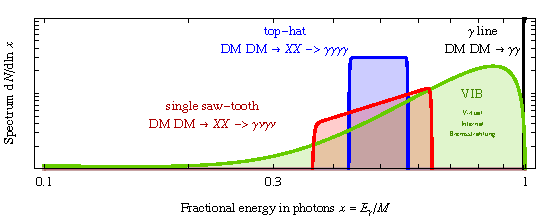
\includegraphics[width=0.75\textwidth]{figs/DMphotonSpectra}$$
\caption[Prompt $\gamma$ spectra]{\em\label{fig:DMphotonSpectra} 
Illustration of notable $\gamma$-ray {\bfseries spectral features} possibly produced by DM annihilation or decays. }
\end{figure}


\subsection{Sharp spectral features in prompt $\gamma$-rays}\label{sec:modeldepgammas}
The annihilations (or decays) of DM particles in specific channels or in specific models can generate distinct, sharp features in the spectra of the produced gamma-rays~\cite{sharpfeatures}. These features are potentially useful for detection because they can be easily distinguished from the predicted astrophysical  background,
especially since, unlike charged cosmic rays, the features in the gamma-ray spectra are not deformed by astrophysical propagation. 
In this subsection, we focus on DM annihilation for the sake of simplicity, but a completely analogous discussion would apply to the case of DM decay, with corresponding adjustments to the $\gamma$-ray energies.

\medskip

The simplest of these features is a {\bf gamma-ray line}, i.e.,~a monochromatic spectrum with a fixed energy, depicted by the black line in fig.~\ref{fig:DMphotonSpectra}. Such a line can be produced, for example, by the process DM DM $\to \gamma \gamma$. 
Since the DM particles are almost at rest in the galactic and cosmological environments (being cold), they possess negligible kinetic energy, and thus the emitted line is at the energy
\beq
E_\gamma = M.
\eeq
For heavy DM the electroweak emissions (see section \ref{sec:EWemissions}) smear the peak of the `delta function', and, more importantly, introduce an additional continuum at $E_\gamma \ll M $. 
These effects are visible in the example spectrum in fig.~\ref{fig:spectraatproduction} (dotted black line). 
As already mentioned above, DM annihilations into photons
occur only via some subdominant mechanism, typically 
 involving charged particle loops,
resulting in a smaller cross section (often reduced by a loop factor) compared to direct annihilation. This renders the detection more challenging.
Nevertheless, the spectral feature is so pronounced that the monochromatic $\gamma$-ray line has been regarded for a long time as the `smoking gun' for DM detection. For a real-world example, see section~\ref{sec:135GeVline}.


\smallskip

In most models, the loop of charged particles mediating the DM DM $\to \gamma \gamma$ process allows to replace one of the $\gamma$ with another neutral SM particle in the final state, e.g.,~a $Z$ or a Higgs boson. 
Due to the finite masses of $Z$ and $h$, this leads to additional $\gamma$-lines at lower energies,
\beq
E_\gamma = M  \left(1- \frac{M^2_{Z, h}}{4 M} \right).
\eeq

\smallskip
Another distinct feature in $\gamma$ rays is produced by \textbf{Virtual Internal Bremsstrahlung (VIB)}, which arises when a photon is emitted from a virtual charged particle that mediates DM annihilation. 
By bringing the charged particle's propagator closer to being on-shell, 
VIB favors the emission of higher-energy photons around the maximal photon energy $E_\gamma\circa{<} M$,
particularly when the charged particle's  mass is not very different from the DM mass.
Consequently, the VIB spectrum exhibits a triangular shape: rising up to a sharp cut-off at an energy corresponding to $M$, as illustrated by the green curve in fig.\fig{DMphotonSpectra}. 
In addition, VIB turns the annihilation into a three-body process, thereby eliminating the helicity suppression when present.
This can be phenomenologically very important in certain cases, with 
the VIB cross section much higher than the cross section for the tree-level 2-body annihilation.






\medskip

A DM that annihilates into two metastable bosons $X$ with mass $m_X$, which subsequently decay into photon pairs 
($\hbox{DM DM} \to X X \to \gamma\gamma\gamma\gamma$),
produces a {\bf `top-hat'} or {\bf `box-shaped'} spectrum. 
The  upper and lower photon energies $E_\pm$ and the width $\Delta E_\gamma$ of this spectrum are given by 
\beq
E_\pm = \frac{M}{2} \left( 1\pm \sqrt{1-\frac{m^2_X}{M^2}} \right), \qquad \hbox{and}\qquad
\Delta E_\gamma = \sqrt{M^2 - m^2_X}.
\label{eq:gammatophat}
\eeq
This is illustrated by the blue curve in fig.\fig{DMphotonSpectra}. 
In the limit where $m_X \circa{<} M$, the phase space becomes restricted, and the spectrum narrows down to a thin line. 


\medskip

A DM that annihilates according to the process $\hbox{DM DM} \to X X \to \gamma \nu \, \gamma \nu$, i.e., 
into two metastable Dirac fermions $X$, which subsequently decay into a photon and another fermionic state (such as~a neutrino), produces a {\bf `single saw-tooth'} spectrum.
This spectrum shares similarities with the top-hat spectrum, but  features a slanted top
(see the red curve in fig.\fig{DMphotonSpectra}).
The slope of the slanted top is determined by the spin polarization of $X$.
The masses must satisfy $M > m_X > m_\nu \approx 0$. The formul\ae\ for the edge energies and the width are the same as those given in  eq.~(\ref{eq:gammatophat}).



\section{Neutrinos}\index{Indirect detection!$\nu$}\index{Neutrino!indirect detection}
\label{sec:neutrinosID}

Neutrinos produced from DM annihilations or decays in either galactic or cosmological environments\footnote{A distinct class of indirect DM searches with neutrinos focuses on the annihilations or decays in the center of the Sun or the Earth. The phenomenology of these searches is entirely different and is covered in detail in section \ref{sec:DMnu}.} 
propagate along nearly straight paths with velocity $v \simeq c$, akin to photons.
Consequently, the discussion of such neutrino signals follows closely 
the discussion of gamma ray signals presented in the previous section. 





The main targets for observation are the Galactic Center, the Galactic Halo, dwarf galaxies, clusters, and the cosmological signal. 
However, not all of these targets are easily accessible due to the significantly more challenging detection of neutrinos compared to photons (see section \ref{sec:IDstatus} for the current status of the searches).
The expected neutrino flux from the Milky Way
can be expressed using equations analogous to eq.s~(\ref{gammaflux}) and (\ref{gammafluxdec}), 
with the same $J$ and $D$ factors. 
Similarly, the ${\mathcal J}$ and ${\mathcal D}$ factors for dwarf galaxies can be described using eq.~(\ref{eq:JdSph}).


\medskip

A notable difference between photons and neutrinos is that the neutrinos undergo flavor oscillations, 
causing the fluxes at detection to differ from those at production.
Given the observed neutrino masses $m_i$ and mixings $V_{\ell i}$,
vacuum oscillations over astrophysical distances $L$ can often be
well approximated by the limit $\Delta m^2 L/E\gg 1$,
where squared oscillation amplitudes are reduced to  classical flavour transition probabilities~\cite{NuOsc}
\begin{equation}
P_{\ell\ell'}=\sum_{i=1}^3 |V_{\ell i} V_{\ell' i} |^2
\approx
\left( 
\begin{array}{ccc}
0.6 & 0.2 & 0.2 \\
0.2 & 0.4 & 0.4 \\
0.2 & 0.4 & 0.4 
\end{array}
\right).
\end{equation}
This means that, for instance, annihilations or decays into $\nu_e$  
produce a flavor composition at detection $(\nu_e : \nu_\mu : \nu_\tau) \sim (0.6 : 0.2 : 0.2)$, 
while the annihilations/decays into either $\nu_\mu$ or $\nu_\tau$ produce $(\nu_e : \nu_\mu : \nu_\tau) \sim(0.2 : 0.4 : 0.4)$. 
Often, for the sake of simplicity,  the assumption is made of democratic composition at detection 
$(\nu_e : \nu_\mu : \nu_\tau) \sim (1 : 1 : 1)$.
This flavour composition is preserved by oscillations
and is also motivated by the fact that a composition close to $(1 : 1 : 1)$ arises, after oscillations, 
if  neutrinos originate from pion decays in the source,
since $\pi^\pm$ decays equally into $\nubarnu_e$ and $\nubarnu_\mu$.

\smallskip

Another hypothetical difference with respect to photons is that neutrinos could interact with DM 
during their galactic or extragalactic propagation. This is addressed in the next subsection.

\subsection{Neutrino/DM interactions?}
\label{sec:neutrinoDMinteractions}
If DM couples to the SM neutrinos, it can leave a discernible imprint in the diffuse flux of high energy neutrinos detected on Earth \cite{DM:nu:interactions}. As extra-galactic neutrinos traverse the galactic plane, they may scatter on the DM in the halo, leading to an attenuation of the neutrino flux.  The most striking effect is obtained if the scattering is through an $s$-channel resonance, $X$, 
\beq
\nu +{\rm DM}\to X^{*}\to \nu +{\rm DM}.
\eeq
The resonance $X$ with mass $m_X$ is produced on-shell if the neutrino has the energy 
\beq
E_\nu^*=\frac{m_X^2-M^2}{2M}=5\, 10^3\, \text{TeV}\,\frac{m_X^2-M^2}{\big(10\,\text{GeV}\big)^2}\biggr(\frac{10\,\text{keV}}{M}\biggr),
\eeq
when it annihilates with the non-relativistic DM in the halo. For neutrino energies $E_\nu\simeq E_\nu^*$ the scattering cross section is resonantly enhanced, and thus the neutrino flux on Earth should exhibit a distinctive dip at the neutrino energy $E_\nu^*$, if DM couples to neutrinos. In contrast, for a $t$-channel resonance there is no distinctive dip in the neutrino spectrum since such scatterings do not lead to a resonantly enhanced cross section. 
 However, if the scattering cross-section is sufficiently large, the neutrino signal will still be attenuated in the direction of the galactic center, where the DM density is highest.

\smallskip

Neutrinos reaching Earth with energies greater than $E_\nu\gtrsim 200$ TeV are considered to be of extragalactic origin. 
The {\sc IceCube} collaboration measured the flux of these extra-galactic neutrinos up to PeV energies,
without observing any distinctive dip or angular dependence in the incoming neutrino flux.  
This allows one to place limits on the DM/neutrino couplings, $g\lesssim 0.01-1$, for 
$100\ \text{keV} \lesssim M\lesssim \GeV$  and  
$1\ \text{keV} \lesssim m_X  \lesssim 100\ \GeV$, 
depending on the details of the interaction model~\cite{DM:nu:interactions}. 
At energies $E_\nu\lesssim 200$ TeV, neutrinos are mostly atmospheric, i.e. generated in the atmosphere of the Earth by incident cosmic rays, and therefore carry no information about DM--neutrino interactions. An exception are neutrinos from supernov\ae, whose flux can emerge from the atmospheric background in a specific energy range around 10-100 MeV. Data from {\sc SuperKamiokande} on SN1987A and on the (galactic) diffuse supernova background can indeed be used to constrain $\sigma_{{\rm DM}-\nu} \lesssim 10^{-24}$ cm$^2$/GeV for $M\gtrsim 1$ GeV~\cite{DM:nu:interactions}.

In 2018 {\sc IceCube} detected a 290 TeV neutrino event from an identified source, the distant flaring blazar TXS 0506+056. For this event to have been observed the neutrino had to cross a large column density of DM between the source and the site of detection, due to both the cosmological and the galactic DM distributions, as well as from the dense DM  spike presumably surrounding the blazar. This can then be used to place bounds on  DM/neutrino interactions~\cite{DM:nu:interactions}.



\section{Positrons and electrons}\label{sec:e+e-}\index{Indirect detection!$e^\pm$}\index{Positron!indirect detection}
In this section, we focus on the computation of the flux of electrons\footnote{We recall that, as discussed in the introduction of this chapter, {\em anti}-matter particles are of particular interest for DM searches. However, the flux of electrons  from DM annihilation/decay has also been considered as a useful quantity, since the flux of electron from other sources is not overwhelmingly larger than that of positrons (see, e.g., fig.~\ref{fig:CRdata}).  Furthermore, a combined electron$+$positron flux is relevant for the experiments that cannot discriminate between charges. It is therefore pertinent to include electrons in the discussion.}
 and positrons from DM annihilations or decays. 
Electrons and positrons detected on Earth originate from the local galactic environment and undergo a complex propagation process within that environment. 
The higher their energy, the closer the sources need to be: 
as a rule of thumb, 50\% (90\%) of 1 GeV (1 TeV) positrons come from within 1 kpc, 
see, e.g.,~\arxivref{0809.5268}{Delahaye et al.~(2009)} in \cite{CRpropagation}.
Dedicated numerical codes such as {\tt Galprop}, {\tt Dragon}, {\tt Picard}, and {\tt Usine}~\cite{CRcodes} have been developed and refined to model the propagation of `ordinary' cosmic rays (CRs), i.e., those of astrophysical origin, and can be adapted for use with DM-produced CRs.
DM oriented codes such as {\tt MicrOMEGAs}~\cite{1801.03509}, {\tt MadDM}~\cite{1804.00044} or {\tt DarkMatters}~\cite{2408.07053} are often interfaced with the codes above and also efficiently do the job.
We highlight the main physics involved in the propagation process and review an approximate semi-analytic solution frequently used in DM indirect detection.
This approach allows for efficient and reliable computation of predicted CR fluxes from DM. 
Comparisons with data can be performed either using the approximate solutions or with the dedicated numerical codes mentioned earlier, though it is crucial to recognize that significant uncertainties may exist, as addressed later in this section.
 While our discussion is mainly centered on electrons and positrons, we will occasionally introduce a more general formalism for future reference.

\smallskip

The DM-induced differential $e^\pm$ flux\footnote{With the notation $e^\pm$ we always refer to the independent fluxes of electrons $e^-$ or positrons $e^+$, which share the same formalism, and not to their sum (for which we use the notation $e^++e^-$ when needed).
The $e^\pm$ fluxes and the $e^++e^-$ flux induced by DM differ by a factor 2, up to possible C violations.} per unit of energy  at any spatial point $\vec x$ and time $t$ is given by $d\Phi_{e^\pm}(t,\vec x,E) /dE\, = v_{e^\pm} f/4\pi$, with units $(\GeV\cdot{\rm cm}^2\cdot{\rm s}\cdot{\rm sr})^{-1}$.
Here, $v_{e^\pm}$ is the velocity  of electrons/positrons, essentially equal to the speed of light $c$ in the regime of weak-scale DM. 
The $e^\pm$ number density per unit energy, $f(t,\vec x,E)= dn_{e^\pm}/dE$,
obeys the diffusion-loss equation in galactic cylindrical coordinates
\beq 
\label{eq:diffeq}
\frac{\partial f}{\partial t}-
\nabla\left( \mathcal{K}(E,\vec x) \nabla f \right) + \frac{\partial}{\partial z}\left( {\rm sign}(z)\, f\, V_{\rm conv} \right) 
- \frac{\partial}{\partial E}\left( b_{e^\pm}(E,\vec x) f + v_{e^\pm}^2 \mathcal{K}_{p}(E,\vec x) \frac{\partial f}{\partial E} \right) = Q(E,\vec x).
\eeq
This equation governs the evolution of the $e^\pm$ number density with an injection rate $Q$, taking into account the various propagation processes that will be discussed shortly.
It is derived from the full general formalism that provides a detailed description of CR transport in the galaxy (for classic references, see \cite{CRtransport}). It is somewhat simplified by retaining only the terms most relevant to $e^\pm$. Furthermore, since steady state conditions hold, the first term in eq.\eq{diffeq} vanishes, and the dependence on time disappears. The other terms are as follows. 

\begin{itemize}

\item[$\triangleright$] DM DM annihilations or DM decays 
 provide the spatially dependent {\bf source term} $Q$ in eq.~(\ref{eq:diffeq}), 
\beq 
\label{eq:QDMpositrons}
Q = \begin{cases}
\displaystyle \frac{1}{2} \left(\frac{\rho}{M}\right)^2 \langle \sigma v \rangle_{\rm tot} \frac{dN_{e^\pm}}{dE} & \text{(DM annihilation),} \\[4mm]
\displaystyle \frac{\rho}{M } \Gamma_{\rm tot} \frac{dN_{e^\pm}}{dE} & \text{(DM decay),}
\end{cases}
\eeq
where the $dN_{e^\pm}/dE$ spectra are given in eq.~(\ref{eq:primaryflux}), and  $\rho(\vec x)$ is the DM density. That is, DM acts as a diffuse source of $e^\pm$, encompassing the entire DM halo. The intensity is higher at the center and diminishes towards the periphery, modulated by $\rho$ (in the case of DM decays) or $\rho^2$ (in the case of DM annihilations). 




\item[$\triangleright$] {\bf The diffusion coefficient} function $\mathcal{K}$ describes the `random walk' diffusion 
of $e^\pm$ as these move in the inhomogeneous turbulent magnetic fields in the galaxy. 
The diffusion coefficient depends on the momentum $p$ of the propagating electron or positron, and thus also on its energy $E$,  
being very crudely proportional to the gyro-radius $\sim p/eB$, where $B$ is the average magnetic field.\footnote{More refined descriptions of the galactic magnetic field are possible, for instance including a regular component in addition to the turbulent one. See e.g.~\arxivref{1904.08160}{Kachelriess and Semikoz (2019)} in \cite{CRtransport}. This leads to a more complex description of diffusion, in general not isotropic.}
While in principle $\mathcal{K}$ may vary with position $\vec{x}$, since the distribution of diffusive inhomogeneities changes throughout the galactic halo, the mapping of such variations remains substantially unknown. For example, the diffusion properties could differ inside and outside the galactic arms, as well as inside and outside the galactic disk, subject to the poorly understood local galactic geography. 
Moreover, including spatial dependence in $\mathcal{K}$ would make the semi-analytic methods much more difficult to implement numerically. 
Therefore, it is customary to treat $\mathcal{K}$ as a scalar and to disregard the spatial dependence, resulting in $\nabla\big( \mathcal{K}(E) \, \nabla f \big) = \mathcal{K}(E) \, \nabla^2 f$.

Several models have been proposed to describe the dependence of the diffusion coefficient $\mathcal{K}$ on energy $E$.
The simplest parameterisation, routinely used in earlier studies, is given by 
\beq
\mathcal{K}(E)=\mathcal{K}_0 \, v_{e^\pm}\, (E/\GeV)^\delta,  
\label{diffcoeffsimple}
\eeq
where $\mathcal{K}_0$ is a normalization factor and $\delta \sim 0.5-1 $ is a diffusion spectral index. 
More recently, a refined parameterization reflecting the observed spectral breaks in CR fluxes \cite{CRbreaks} has been adopted. 
When generalized to any charged CR with charge $Ze$, 
and formulated in terms of rigidity $R \equiv p/Ze$ rather than energy, it takes the form 
\beq
\mathcal{K}(R) = v^\eta \, \mathcal{K}_0 \left(\frac{R}{1 \, {\rm GV}} \right)^\delta \left[1+ \left( \frac{R_l}{R} \right)^{(\delta-\delta_l)/s_l} \right]^{s_l}
 \left[1+ \left( \frac{R}{R_h} \right)^{(\delta-\delta_h)/s_h} \right]^{-s_h}.
\label{diffcoeffbreaks}
\eeq
Here, the parameters $R_{l(h)}$ indicate the positions of the spectral breaks, $\delta_{l(h)}$ denote the diffusion spectral indices in the low- and high-rigidity regime, respectively, and $s_{l(h)}$ characterises the rate at which the spectral change takes place around $R_{l(h)}$. In the  relativistic $e^\pm$ limit, and ignoring the spectral breaks,
the formalism simplifies to the original parameterisation in eq.~(\ref{diffcoeffsimple}).
The values of all these parameters will be the focus of a dedicated discussion below.


\item[$\triangleright$] The $\mathcal{K}_{p}$ term in eq.\eq{diffeq} accounts for the so-called {\bf reacceleration}, i.e.,~the process in which the propagating particles hit the diffusion centers (i.e.,~the knots of a turbulent galactic magnetic field) and undergo a second-order Fermi acceleration. That is, the diffusion centers, which are drifting at a certain speed, cause the particles to gain energy. 
Spatial diffusion thus also leads to a modification of the energy of the propagating cosmic ray and therefore to a {\em diffusion in momentum space}. One way to parametrise the diffusive re-acceleration coefficient is 
\beq
\label{eq:reaccelerationcoeff}
\mathcal{K}_{p}(E,\vec x) = \frac43 \frac{V_a^2}{\mathcal{K}(E,\vec x)} \frac{p^2}{\delta (4-\delta^2)(4-\delta)},
\eeq
where $V_a$ is an effective Alfv\'enic speed, a property of the magnetic turbulence centers, and $\delta$ is the spectral index of spatial diffusion, introduced earlier. The dependence of $\mathcal{K}_{p}$ on the inverse of the spatial diffusion coefficient $\mathcal{K}$ encodes the fact that the more efficiently cosmic rays diffuse in space, 
the fewer collisions occur, thereby weakening the energy diffusion process.



\item[$\triangleright$] The $V_{\rm conv}$ term represents a {\bf convective wind}, assumed to be constant and directed outward from the galactic plane. 
This wind exerts a force on charged cosmic rays, pushing them away from the galactic plane. Its impact is higher on low energy particles ($E \lesssim$ few GeV) due to their lower rigidity.  More refined scenarios with $V_{\rm conv}$ that is not constant, but rather increases or decreases with $z$, have also been considered.



\item[$\triangleright$] \index{Positron!energy loss}
The {\bf $e^\pm$ energy loss coefficient function} $b_{e^\pm}(E, \vec x)$ 
quantifies the energy losses experienced by the $e^\pm$ during their propagation. 
In general, it depends on the position $\vec x$, 
reflecting the fact that energy losses are influenced by the specific environment. It also depends on the energy $E$ of the propagating $e^\pm$. 
Various mechanisms contribute to these losses, including energy dissipation through Coulomb interactions and ionization with the interstellar gas, bremsstrahlung on the same gas, Inverse Compton Scattering (ICS) on the InterStellar Radiation Field (ISRF), and synchrotron emission in the galactic magnetic field. 
Schematically, the total energy loss can be expressed as
\begin{equation}
\label{eq:btot}
b_{e^\pm}(E,\vec x) \equiv -\frac{{\rm d}E}{{\rm d}t} = b_{\rm Coul+ioniz} + b_{\rm brem} + b_{\rm ICS} + b_{\rm syn}.
\end{equation}
The processes above are listed in order of increasing relevance as the $e^\pm$ energy increases.  
For detailed expressions of these terms and further insights into their underlying physics, the reader is referred to the relevant literature \cite{CRenergylosses,PPPC4DMID}\footnote{The reader can also consult section \ref{sec:secondary photons}, where some of these same processes are considered for the emission signals they produce.}, while here we just sketch their main features:

\begin{itemize}
\item {\em Coulomb interactions and ionizations of the gas} are primarily relevant for $e^\pm$ with energies $E \lesssim 1$ GeV.\footnote{These ranges are only indicative: the specific details depend on the local density of gas and radiation, as well as the intensity of the magnetic field where the interactions happen, and their relative weight in the impact for energy loss. These ranges are roughly correct for the environment around the solar system.} They occur on neutral and ionized galactic gas, with Thompson cross section $\sigma_{\rm T} = 8\pi  r_e^2/3$, where $r_e = \alpha/m_e$ is the classical electron radius, inversely proportional to the electron mass $m_e$. 
The energy losses are proportional to the density of target atoms and molecules, necessitating detailed spatial maps that are often deduced from external astrophysical observations. The energy loss rate $b_{\rm Coul+ioniz}$ due to these processes is roughly independent of the $e^\pm$ energy.

 
\item {\em Bremsstrahlung interactions} are relevant in the range $1 \ {\rm GeV} \lesssim E \lesssim 10$ GeV.  Like Coulomb interactions and ionizations, they occur on neutral and ionized galactic gas too. The relevant cross section contains again the Thompson cross section and an additional factor of $\alpha$ associated to the bremsstrahlung photon emission. The energy loss rate $b_{\rm brem}$ is linearly dependent on $E$. 


\item {\em ICS processes} are dominant for $10 \ {\rm GeV} \lesssim E \lesssim 100$ GeV. They occur on the three main components of the ISRF: 
optical star-light, dust-diffused infrared light and the CMB, the latter being a black body spectrum with temperature $T=2.725$ K. 
For the optical and infrared components, detailed maps are required for a precise description.
The energy dependence of ICS losses is described by $b_{\rm ICS} \propto E^2$, valid in the non-relativistic Thomson regime.\footnote{The Thomson regime in electron-photon Compton scattering is characterized by the condition  $\epsilon^\prime_{\rm max} = 2 \gamma \epsilon < m_e$, where $\epsilon$ denotes the energy of the impinging photon, $\epsilon^\prime$ the same quantity in the rest frame of the electron, while $\gamma$ is the Lorentz factor of the electron. 
When $e^\pm$ scatter on CMB photons ($\epsilon \approx 2\ 10^{-4}$ eV) this condition is satisfied up to $\sim$ TeV $e^\pm$ energies. For scatterings on more energetic starlight ($\epsilon \approx$ 0.3 eV), the condition breaks down already above $e^\pm$ energies of $\approx$ few GeV.} 
For sufficiently high electron energy, the IC scattering enters the relativistic regime, where the $\gamma e^\pm$ Klein-Nishina cross section becomes smaller than in the Thomson limit.
Consequently, a multiplicative factor $R_i^{\rm KN}(E) < 1$ must be introduced (see, e.g., fig.~2 of \arxivref{0905.0480}{Meade et al.~(2010)} in \cite{CRenergylosses}, and eq. \eqref{eq:b(E)} below), leading to a reduction in $b_{\rm ICS}(E)$.



\item {\em Synchrotron emission} becomes the dominant channel of energy loss for high-energy electrons and positrons. 
This process depends on the intensity of the galactic magnetic field at $\vec x$, a quantity that is rather uncertain \cite{Bgaldeterminations}. \label{Bgalactic}
Generally speaking, in spiral galaxies like the Milky Way, 
the strength of the total magnetic field is expected to be of the order of 10 $\mu$G $-$ 1 mG and to follow the spiral pattern. 
Measurements specific to the Milky Way indicate a value around 5$-$6 $\mu$G at the position of the Sun and $10-40~ \mu$G close to the Galactic Center. 
 The intensity of the galactic magnetic field is typically modeled with a profile that peaks at the galactic center and decreases with smooth exponents in both the radial and vertical directions. 
\label{galacticB} More detailed profiles, which take into account the galactic morphology of arms and voids, are also sometimes used. 
The energy dependence of synchrotron emission losses is given by $b_{\rm syn} \propto E^2$.
\end{itemize}

The summary result for the function $b_{e^\pm}(E,\vec{x})$ is illustrated in fig.~\ref{fig:b}.
In the figure, 
the $E^2$ behavior at intermediate energies is apparent.
 At low energies, the dependence softens, since the Coulomb, ionization and bremsstrahlung losses dominate. 
 At high energies, the dependence also softens because of the Klein-Nishina effect.
 The transition happens earlier at the GC, where star-light is more abundant, and later at the periphery of the Galaxy, where the CMB is the dominant background. 
At the GC, the dependence eventually
re-settles onto an $E^2$ slope at very high energies, where synchrotron losses dominate.  


\begin{figure}[!t]
\begin{center}
\hspace{-1.3cm}
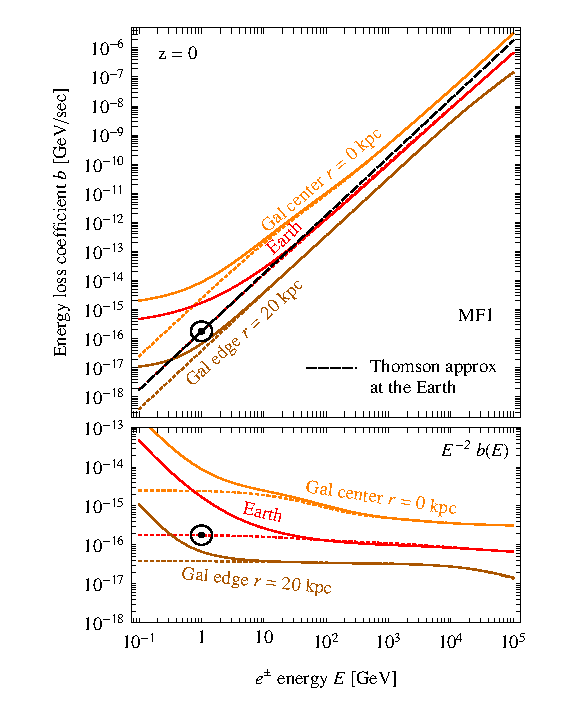
\includegraphics[width= 0.55 \textwidth]{figs/b}
\hspace{-0.9cm}
 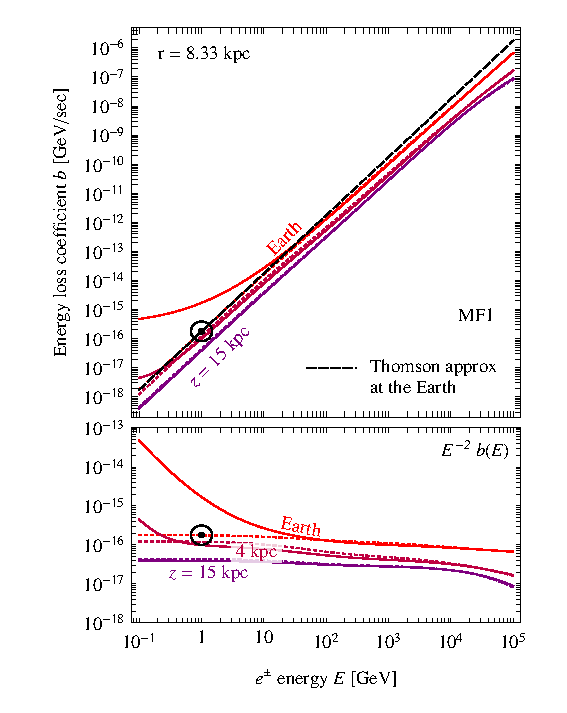
\includegraphics[width= 0.55 \textwidth]{figs/bz}
\caption[Energy loss of $e^\pm$ in the Milky Way]{\em \small \label{fig:b} {\bfseries Energy loss coefficient function} for electrons and positrons in the Milky Way. Left panel: in the galactic disk ($z = 0$), at several locations along the galactic radial coordinate $r$. Right panel: above (or below) the location of the Earth along the coordinate $z$. 
Here MF1 denotes a choice for the galactic magnetic field. 
The circled dot identifies the constant value $\tau_\odot$ sometimes adopted. 
The dotted colored lines are the same function neglecting the low energy losses (essentially Coulomb, ionization and bremsstrahlung), and the black dashed line corresponds to adopting the Thomson approximation (i.e.~neglecting the Klein-Nishina factor) for the ICS losses. The lower panels show the same function divided by $E^2$, to highlight the deviations from a simple $E^2$ behaviour. Figure adapted from \arxivref{1505.01049}{Buch et al.~(2015)} in~\cite{CRenergylosses}.}
\end{center}
\end{figure}
\end{itemize}


The low-energy losses are often neglected when the focus is on energetic $e^\pm$ originating from
weak-scale DM. 
In such cases, the energy loss can be approximated by
\beq\label{eq:b(E)}
 b_{e^\pm}(E,\vec x) \approx b_{\rm ICS}(E,\vec x) + b_{\rm syn}(E,\vec x) =  \frac{4\sigma_{\rm T} }{3 m_e^2}  
 E^2  \tilde{u}, \qquad 
\tilde{u}= \sum _i u_{\gamma}(\vec x)  R_i^{\rm KN}(E) +  u_B(\vec x),  \eeq
where $u_B = B^2/2$ is the energy density in galactic magnetic fields of intensity $B$ and $u_{\gamma,i} = \int dE_\gamma\, n_i(E_\gamma)$ is the energy density in light, 
summed over the three main components of the ISRF with photon number densities $n_i$. 
An even further approximation can be made by neglecting the spatial dependence in $b_{e^\pm}$ and ignoring the Klein-Nishina suppression in the ICS processes. This leads to
\beq
\label{eq:bT(E)}
b_{e^\pm}(E) \approx \frac{E^2}{{\rm GeV} \ \tau_\odot}  \equiv b_{\rm T}(E),
\eeq
where $\tau_\odot = 5.7 \ 10^{15}$ sec is characteristic of the $e^\pm$ energy losses at the location of the solar system, in this rather drastically simplified scenario.

\medskip

In semi-analytic solution methods, which are also employed by most of the numerical codes referenced earlier,
eq.~(\ref{eq:diffeq}) is solved within a specific diffusive region. 
This region is assumed to be a flat cylinder with the galactic plane at its symmetry plane, and has a height of $2L$ in the $z$ direction and a radius $R = 20\, {\rm kpc}$ in the $r$ direction~\cite{CRpropagation}.\footnote{This configuration is referred to as the {\em two-zone diffusion model}: one zone is the diffusive cylinder, the other the thin galactic disk containing the gas (see below).}
 The location of the solar system is given by the coordinates $(r_{\odot}, z_{\odot}) = (8.33\, {\rm kpc}, 0)$.
The cylindrical region represents the space where charged particles are presumed to remain confined by the magnetic field, and its shape is inspired by (mostly radiowave) observations of external galaxies.  
Mathematically, this means that the boundary conditions are imposed in such a way that the $e^\pm$ density $f$ vanishes on the surface of the cylinder, outside of which electrons and positrons propagate freely and escape. 




\medskip

Stepping back, our extensive discussion above highlights that the propagation of electrons and positrons is a complex process, influenced by numerous astrophysical phenomena. 
Specifically, the propagation relies on several \emph{propagation parameters} present in the preceding equations. 
These parameters, in order of their introduction, are: $\eta, \mathcal{K}_0, \delta, R_l, \delta_l, s_l, R_h, \delta_h, s_h, V_a, V_{\rm conv},$ and $L$.
Some of these parameters have a large impact on the resulting fluxes of electrons and positrons (as well as anti-protons and anti-nuclei, discussed in the following sections). 
For instance, the height of the diffusive cylinder $L$ determines how tall is the confinement region. 
 Intuitively, a larger $L$ leads to more extensive confinement, resulting in a higher final flux, especially as positrons originating from as far as the dense regions close to the GC remain confined, and thus can potentially be detected on Earth. 
Conversely, some parameters exert minimal influence or are strictly constrained by other observational data.\footnote{
Additionally, there are interdependences between the parameters describing the astrophysical ingredients. For instance, the thickness $L$ of the CR diffusive halo is related to the vertical extent of the galactic magnetic field discussed on page \pageref{galacticB}. However, such correlations are often neglected for simplicity, at least in the DM-related CR literature.
} 

A significant branch of CR research over past decades has been dedicated to determining these parameters using a combination of `ordinary'  CR data and models (i.e.,~not related to DM), particularly through secondary-to-primary CR ratios (conventionally, the most used  is the boron-to-carbon (B/C) ratio). 
More precisely, one first identifies a {\em propagation scheme}, i.e.,~a version of the full transport equation~(\ref{eq:diffeq}), 
either including or omitting individual components, and subsequently identifies plausible ranges for the retained propagation parameters.
For concreteness, we will follow the state-of-the-art analysis by \arxivref{1904.08917}{G\'enolini et al.~(2019)} in \cite{CRpropagation}, which takes advantage of the high-precision CR data provided by the {\sc Ams}-02 experiment. 
They selected three propagation schemes termed \texttt{BIG}, \texttt{SLIM} and \texttt{QUAINT}:
\begin{itemize}
    \item[$\blacktriangleright$]
\texttt{BIG} is the most complete and versatile: it includes a double-break diffusion coefficient as in eq.~(\ref{diffcoeffbreaks}), as well as convection and re-acceleration, with all the corresponding parameters.
    \item[$\blacktriangleright$] 
 \texttt{SLIM}    is a minimalistic version of the former: it does not include convection nor re-acceleration (i.e.~$V_{\rm conv} = V_a = 0$) and fixes $\eta =1$.
 \item[$\blacktriangleright$]
 \texttt{QUAINT} includes convection and re-acceleration but does not include a low-energy spectral break. 
 \end{itemize}
For each of these schemes, specific parameter sets were identified, with table~\ref{tab:proparam} showing parameters for the \texttt{SLIM} configuration as an example. 
These sets either maximize or minimize the resulting fluxes of DM-related cosmic rays at Earth.\footnote{Note that these parameters do not necessarily correspond to the same extremal fluxes in other locations of the Galaxy. 
For instance, the MAX set leads to the most suppressed flux of positrons in some areas near the GC, 
while MIN and MED yield the most enhanced one. 
This variability stems from the differing relative significance of the propagation parameters, which varies between the Earth's vicinity and other galactic locations.
} 
They are thus named MIN, MED, and MAX.
Other similar sets have been considered in the past. 
Works by  \arxivref{astro-ph/0306207}{Donato et al.~(2004)}
and \arxivref{0809.5268}{Delahaye et al.~(2008)} in~\cite{CRpropagation}  introduced the original versions of the MIN-MED-MAX sets, now updated by those in table~\ref{tab:proparam}. 
Additionally, alternative sets have been proposed by, among others,  
\arxivref{0909.4548}{Di Bernardo et al.~(2010)}, \arxivref{1210.4546}{Di Bernardo et al.~(2013)} and 
\arxivref{1011.0037}{Trotta et al.~(2011)} in~\cite{CRpropagation}.



\begin{table}[t]
\center
\begin{tabular}{c|ccccc}
  & $\delta$ & $\mathcal{K}_0$ in kpc$^2$/Myr & $R_l$ in GV & $\delta_l$ & $L$ in kpc  \\
\hline 
MIN  & 0.509 & 0.01945 & 4.21 & $-1.450$ & 2.56  \\
MED & 0.499 & 0.03631 & 4.48 &  $-1.110$ & 4.67  \\
MAX  & 0.490 & 0.06607 &  4.74 &  $-0.776$ & 8.40 
\end{tabular}
\caption[Propagation of charged particles in the Milky Way]{\em \small {\bfseries Propagation parameters} for charged particles in the Galaxy, for the \texttt{SLIM} propagation scheme. The values of the fixed parameters, for this scheme, read $\eta =1, s_l = 0.05, R_h = 237 \ {\rm GV}, \delta_h = \delta -0.19, s_h =0.04, V_{\rm conv} = V_a = 0$. The values are from \arxivref{2103.04108}{G\'enolini et al.~(2021)} in \cite{CRpropagation}, where equivalent sets for other propagation schemes are given. 
\label{tab:proparam}}
\end{table}


\medskip

In summary, setting the parameters in eq.~(\ref{eq:diffeq}) to their values in table~\ref{tab:proparam} (or to other estimates), and then solving this equation either through semi-analytic or numerical methods, one can calculate the DM annihilation/decay induced fluxes of electrons and positrons at Earth, after their propagation through the Galaxy. 





\subsection{Semi-analytic solution via halo functions}\index{Propagation function!$e^\pm$}
\label{sec:epemhalofunctions}
It is instructive to examine an explicit solution method within a simplified context. 
Let us choose the simplest version of the diffusion coefficient, eq.~(\ref{diffcoeffsimple}), neglect the terms for convection and re-acceleration and adopt the simplified form of the energy loss function $b_{\rm T}(E)$ as in eq.~(\ref{eq:bT(E)}). 
Under these assumptions, it is possible to demonstrate \cite{CRpropagation} that the solution to eq.~\eqref{eq:diffeq} can be expressed as
\beq
\label{eq:positronsfluxnox}
\frac{d\Phi_{e^\pm}}{dE}(E,\vec{x}) = \frac1{4\pi}\frac{v_{e^\pm}}{b_{\rm T}(E)}\left \{
\begin{array}{ll}
\displaystyle \frac12 \left(\frac{\rho_\odot}{M}\right)^2  \int_E^{M} dE_{\rm s}\  \langle \sigma v \rangle_{\rm tot} \, \frac{dN_{e^\pm}}{dE}(E_{\rm s}) \ \mathcal{I}(\lambda_D(E,E_{\rm s}),\vec x) & {\rm (DM~annihilation),} \\[5mm]
\displaystyle \left(\frac{\rho_\odot}{M}\right)  \int_E^{M/2} dE_{\rm s} \ \Gamma_{\rm tot} \, \frac{dN_{e^\pm}}{dE}(E_{\rm s}) \ \mathcal{I}(\lambda_D(E,E_{\rm s}),\vec x) & {\rm (DM~decay).}
\end{array}
\right. 
\eeq 
That is, the solution can be written as a simple convolution between the spectra at production $dN_{e^\pm}/dE$ and a dimension-less
{\em halo function} $\mathcal{I}(\lambda_D, \vec x)$ 
that depends on a single quantity
\beq 
\lambda_D = \lambda_D(E,E_{\rm s}) = \sqrt{4\mathcal{K}_0 \tau_\odot [E^{\delta-1} - E_{\rm s}^{\delta-1}]/(1-\delta)},
\eeq 
which represents the diffusion length of $e^\pm$ injected with energy $E_{\rm s}$ and detected with energy $E$. 
 The halo functions essentially act as Green's functions from a source with fixed energy $E_{\rm s}$ to any energy $E$. 
They obey the differential equation
$\nabla^2\mathcal{I} - (2/\lambda_D) \partial \mathcal{I}/\partial\lambda_D=0$, 
derived from eq.~(\ref{eq:diffeq}), to be solved with 
$\mathcal{I} =0$ on the boundary of the cylinder and the initial
condition
$\mathcal{I} (0,\mb{x})= [\rho(\mb{x})/\rho_\odot]^p$ (with $p=2$ for DM annihilations, and $p=1$
for DM decays).
Examples of solutions are shown in fig.\fig{HaloFunctionElectron}: the halo functions can 
exceed 1 if containment within the galactic magnetic field enables the collection of $e^\pm$ from denser and more distant regions toward the Galactic Center (GC), thereby enhancing the fluxes.



  
Reverting to the complete form of the energy loss function, eq.~(\ref{eq:b(E)}), one can generalize the above formalism and compute {\em generalized halo functions} $I(E, E_{\rm s}, \vec x)$,
which serve the same purpose as the $\mathcal{I}$ functions (see \cite{PPPC4DMID} and 
\arxivref{1505.01049}{Buch et al.~(2015)} in~\cite{CRenergylosses}). 
For the full technical details, we refer the reader to the relevant literature. 
It is worth emphasizing that the 'halo function formalism' has limitations, as it fails to capture the full complexity of galactic propagation, particularly at low energies where specialized codes are required. Nevertheless, it remains a practically convenient method, enabling the calculation of propagated cosmic ray fluxes through a straightforward integration over the source energy.
 The halo functions $\mathcal{I}$ encapsulate all the astrophysical considerations (with a distinct halo function $\mathcal{I}$ for each choice of DM distribution profile and $e^\pm$ propagation parameters) and are independent of the specific  particle physics model. Convoluted with the injection spectra, they give the final spectra after galactic propagation. 

\medskip

\label{solar_modulation}
The final step in obtaining spectra that are directly comparable to observational data consists of taking into account the effect of {\bf solar modulation} \cite{SolarMod}.
The solar wind and the solar magnetic field  affect significantly the trajectory of charged cosmic rays as they approach the solar system, particularly those with energies below a few GeV.
The process is treated effectively, in the so-called {\em force field approximation}, 
where it is assumed that solar activity reduces the energy and momentum of charged cosmic rays.
The energy spectrum $d\Phi_{\oplus}/dK_\oplus$ of charged particles reaching the Earth with kinetic energy $K_\oplus$ and momentum $p_\oplus$ (known as the Top of the Atmosphere or `ToA' flux) is approximately related to their energy spectrum in the interstellar medium, $d\Phi/dK$, as  \label{solarmod}
\beq 
\frac{d\Phi_\oplus}{dK_\oplus} = \frac{p_\oplus^2}{p^2} \frac{d\Phi}{dK},\qquad
K= K_\oplus + |Ze| \phi_{\rm Fisk}, \qquad
p^2 = 2m K+K^2,
\eeq
where $m$ and $Z$ denote the mass and charge of the 
CR particles.
The Fisk potential $\phi_{\rm Fisk}$ parameterizes the kinetic energy loss in this effective formalism. Its value depends on the activity of the Sun, which is known to follow  an 11-year cycle, and can be measured in several ways, including using neutron monitors.  
Typical values for $\phi_{\rm Fisk}$ lie between 0.5 GV and 0.9 GV but may range over $0.3-1.3$ GV. 
For instance, $\phi_{\rm Fisk} \approx 0.5\ {\rm GV}$ is characteristic of a minimum of the solar cyclic activity 
(as observed in the second half of the '90s, late 2000s, and around 2020), whereas
$\phi_{\rm Fisk} \gtrsim 0.9\ {\rm GV}$ is typical of a maximum (the early 2000's and the first half of the 2010's), 
see  \arxivref{1607.01976}{Ghelfi et al. (2017)} in~\cite{SolarMod} for a historical overview spanning nearly 70 years.
More refined treatments, and dedicated codes, have been developed \cite{SolarMod}, in particular to take into account possible charge dependencies of the process.


\begin{figure}[t]
$$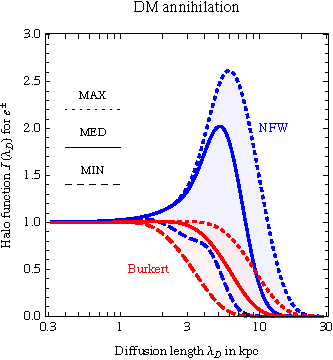
\includegraphics[width=0.4 \textwidth]{figs/HaloFunctionElectronAnn2022}\qquad
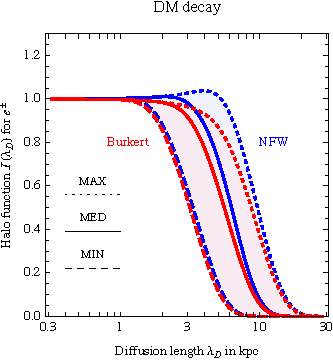
\includegraphics[width=0.4\textwidth]{figs/HaloFunctionElectronDecay2022}$$
\caption[Halo function for $e^\pm$]{\em {\bfseries Halo functions} for $e^\pm$ at Sun's location for the propagation parameters in table~\ref{tab:proparam}
and two DM profiles from table~\ref{fig:DMprofiles}. \label{fig:HaloFunctionElectron} }
\end{figure}



\subsection{Positrons and electrons: practical results}
The above formalism enables the computation of electron and positron fluxes following their galactic propagation, starting from the injection fluxes presented in section \ref{DMspectra} and depicted, e.g.,~in fig.~\ref{fig:spectraatproduction} (left panel). 
The \textbf{broad features} of the resulting fluxes are:
\begin{itemize}
\item[$\circ$] 
The end-point of the spectra remains fixed at $E = M$ (for DM annihilations) or $E = M/2$ (for DM decays). 
However, in cases of strong re-acceleration, a tail of $e^\pm$ with $E >M$ ($E>M/2$) may emerge.
\item[$\circ$] 
The overall normalization of the fluxes is governed by the annihilation cross section $\langle \sigma v \rangle$ (or the decay rate $\Gamma$) and is proportional to the DM density squared $\rho^2$ for DM annihilations (to $\rho$ for DM decays).  
\item[$\circ$] 
Galactic propagation modifies the spectral shape of the fluxes, mostly by redistributing high-energy $e^\pm$ to lower energies, 
though in the case of strong re-acceleration the redistribution to higher energies is also possible.  
The distinctive sharp features characteristic of leptonic channels (see fig.~\ref{fig:spectraatproduction}, left panel) are therefore partially washed out. 
Nevertheless, general characterizations such as
``hard spectrum from leptonic channels'' versus ``soft spectrum from hadronic/gauge boson channels'' 
remain intact.
\end{itemize}

The processes of injection and propagation introduce also notable sources of {\bf uncertainty} in the predicted fluxes. 
These uncertainties can be broadly classified into three categories:
\begin{itemize}
\item[$\triangleright$] \textit{Galactic propagation}. 
This category is defined by sets of parameters like those listed in table \ref{tab:proparam}. 
They represent the current range of sensible possibilities, encompassing the minimal to maximal fluxes predicted from DM  that are compatible with ordinary CR physics.
That is, the allowed values of these parameters serve as an estimate of the present uncertainty related to propagation.
 For $e^\pm$, the impact is energy-dependent. 
 Low-energy $e^\pm$ (e.g.,~$E\sim1-10$ GeV) 
 originate from a large volume
  and are therefore significantly affected by the propagation processes: the span between the MIN and MAX predictions is typically a factor of a few. 
  High-energy $e^\pm$, being more localized, have less uncertain flux. 
In addition, solar modulation, which modifies the CR fluxes at low energies, is subject to large uncertainties.
\item[$\triangleright$] \textit{DM distribution.} 
Uncertainties in the distribution of DM within the Galaxy influence the predicted fluxes.  For $e^\pm$ the impact is energy dependent. For high-energy $e^\pm$, only the local value of the DM density is relevant. For low-energy $e^\pm$, the whole  DM profile is important, including its behavior at the galactic center: the variation in the predicted flux from a cored  to a peaked profile is typically a bit less than an order of magnitude for annihilating DM.
Furthermore, DM over-densities, if present, can boost the flux in the DM annihilation scenario (see section~\ref{sec:astroboost}).
\item[$\triangleright$] \textit{Energy losses.} The densities of interstellar gas and  ISRF as well as  the intensity of the magnetic field enter as external ingredients in the propagation formalism described above. 
The associated uncertainties then translate into 
the predicted CR fluxes. Their detailed impact is location- and energy-dependent, given that the environmental conditions are more uncertain in the inner regions of the Galaxy than they are locally. Roughly, changing the gas and light densities and the magnetic field within currently accepted ranges can alter the final DM $e^\pm$ spectra by a factor of $\sim$2.
\end{itemize}
A summary of the data and its implications for DM will be presented  in section \ref{sec:IDstatus}.



\section{Anti-protons}\label{anti-protons}
\index{Indirect detection!$\bar p$}
\index{Anti-proton}
The propagation of anti-protons\footnote{We recall that, as discussed in the introduction of this chapter, anti-matter particles are of greater interest for DM searches. CR protons from astrophysical sources are so overwhelmingly dominant ($p/\bar p \approx 10^5$ at GeV energies, see, e.g.,~fig.~\ref{fig:CRdata}), that the protons are practically never used for DM searches. Therefore, CR protons are not considered here.} $\bar p$ through the galaxy shares many similarities with that of electrons and positrons discussed in the previous section.  
However, there are also notable qualitative differences, which can be summarized as follows:
\begin{enumerate}
\item[i)]  Energy losses are much less relevant for $\bar p$, leading to better preservation of the spectral shape of the injection fluxes (see below for a detailed discussion). 
On the other hand, different DM annihilation channels tend to give  similar $\bar p$ spectra, see section \ref{DMspectra}. 
Moreover, for a given energy, $\bar p$ have a longer survival time in the diffusive halo compared to $e^\pm$, resulting in  a larger collection volume.
\item[ii)]  Anti-protons are subject to  nuclear physics interactions {\em (spallations)} with the interstellar gas.
 These interactions modify their flux by removing particles (e.g.,~through $\bar p$ annihilation on interstellar hydrogen) or adding particles (e.g.,~through spallations that produce additional $\bar p$). 
\end{enumerate}


\smallskip

The number density of anti-protons per unit energy $f(t,\vec x,K) = dN_{\bar p}/dK$, expressed in terms of the kinetic energy $K=E-m_p$, which is used instead of the total energy $E$,\footnote{This distinction is not particularly relevant for fluxes originating from TeV-scale DM, i.e.,~at energies much larger than the proton mass $m_p$, but it is important for the low energy tails and in the case of small DM masses.} obeys a diffusion equation analogous to eq.~(\ref{eq:diffeq}) \cite{CRtransport,CRpropagation}:
\beq 
\label{eq:diffeqp}
\begin{split}
\frac{\partial f}{\partial t}-
& \mb{\nabla}\cdot \left( \mathcal{K}(K,\vec x) \mb{\nabla} f \right) 
+ \frac{\partial}{\partial z}\left( {\rm sign}(z)\, f\, V_{\rm conv} \right) 
- \frac{\partial}{\partial K}\left(b_{\bar p}(K,\vec x) f + v_{\bar p}^2 \, \mathcal{K}_{p}(K,\vec x) \frac{\partial f}{\partial K}  \right)= 
\\
=& \ Q(K,\vec x)-2h\, \delta(z)\, (\Gamma_{\rm ann} + \Gamma_{\rm non-ann}) f.
\end{split}
\eeq
We refer to the previous section for the common terms, and only comment on the differences.
\begin{itemize}
\item[$\triangleright$] The {\bf source term} $Q$ due to DM DM annihilations or DM decay has a form analogous to eq.\eq{QDMpositrons}, 
with $E$ replaced by $K$ and with the $\bar p$ spectra from eq.~(\ref{eq:primaryflux}). 
DM acts as a diffuse source of $\bar p$, encompassing the entire halo.


\item[$\triangleright$] The pure {\bf diffusion term} is again assumed to be space independent. Its simplest parametrization reads, analogously to eq.~(\ref{diffcoeffsimple}),
\beq
\mathcal{K}(K) = v_{\bar p} \, \mathcal{K}_0 \, (p/\GeV)^\delta,
\label{eq:diffcoeffsimplePbar}
\eeq
where $p = [K^2 +2 m_p K]^{1/2}$ and $v_{\bar p} = [1-m_p^2/(K+m_p)^2]^{1/2}$ are the anti-proton momentum and speed. 
A more refined parametrization, which includes spectral breaks, is as in eq.~(\ref{diffcoeffbreaks}).

\item[$\triangleright$] The {\bf reacceleration} term is analogous to eq.~(\ref{eq:reaccelerationcoeff}). Other terms contributing to reacceleration, that can appear at higher orders, are neglected here.

\item[$\triangleright$] The {\bf energy losses}, expressed by the function $b_{\bar p} (K,\vec x)$, are qualitatively different for anti-protons  in comparison to $e^\pm$. Since $m_p \gg m_e$, the ICS and synchrotron losses, which scale as $1/m^2$, are negligible. 
In fact, all of the energy losses are
not very important for anti-protons and are generally neglected. However, in detailed studies one should still include \cite{Pbarenergylosses}
\beq
b_{\bar p}(K,\vec x) = b_{\rm Coul+ioniz} + b_{\rm adia},
\eeq
where the two terms represent:
\begin{itemize}
\item {\em Coulomb interactions and ionizations} on the interstellar gas, analogous to those for $e^\pm$. These processes are limited to the galactic disk, where the gas is present.\footnote{The (inverse) bremsstrahlung process, where an impinging anti-proton hits an atomic electron at rest, causing the emission of a photon, can also be considered. However, it does not lead to appreciable energy loss for the anti-proton and is therefore neglected.} Therefore, the $b_{\bar p}$ term includes a factor $2 h \, \delta(z)$, which effectively localizes the rate to the $z = 0$ plane. Here, $h \approx 100 \ {\rm pc} \ll L$ is the thickness of the galactic disk. These energy loss processes are still proportional to the Thomson cross section and the number density of gas atoms, but the detailed expressions are somewhat different from those for $e^\pm$ (see, e.g.,~the summary in \arxivref{astro-ph/9807150}{Strong and Moskalenko (1998)} in \cite{Pbarenergylosses}). 
\item {\em Adiabatic losses.} The convective processes encoded in the $V_{\rm conv}$ term induce a loss of energy: 
as the CR are `pushed' by the convective wind, their density decreases, i.e.,~they can be modeled as an expanding gas. 
Without external heat exchange, they then lose energy due to decreasing pressure.
This leads to $b_{\rm adia} = V_{\rm conv} p^2/3h E$. 
\end{itemize}

\item[$\triangleright$]
The last term in eq.\eq{diffeqp} is a {\bf sink term} that removes $\bar p$ from the flux. It accounts for various nuclear physics interactions of anti-protons with the interstellar gas,\footnote{In contrast, the interactions of $e^\pm$ with the gas are negligible and were not included in eq.~(\ref{eq:diffeq}), see 
Gaggero et al.~(2013) in \cite{CRenergylosses} for a quantitative assessment.} which is localized in the galactic disk, hence the factor $2 h \, \delta(z)$. 
\begin{itemize}
\item The first contribution describes the annihilations of $\bar p$ on interstellar protons in the galactic plane, with the rate
$\Gamma_{\rm ann} = (n_{\rm H} + 4^{2/3} n_{\rm He}) \sigma^{\rm ann}_{\bar{p}p} v_{\bar{p}}$,
where $n_{\rm H}\approx 1/{\rm cm}^3$ is the hydrogen density, $n_{\rm He}\approx 0.07\, n_{\rm H}$ is the Helium density (the factor $4^{2/3}$ accounts in an effective way for the differences in geometrical cross-sections).
The cross section $ \sigma^{\rm ann}_{\bar{p}p}$ has been studied in some detail in the literature \cite{Pbarcrosssections}, with the parametrization  introduced by Tan and Ng (1983) still widely used. 

\item The second contribution, similarly, describes the interactions on interstellar protons in the galactic plane in which the $\bar p$'s do not annihilate but lose a significant fraction of their energy. 
In a technical sense, these particles should remain in the flux with degraded energy and
can indeed be considered a form of energy loss, see, e.g,.~\arxivref{1412.5696}{Boudaud et al.~(2015)} in~\cite{Pbarenergylosses}: they are referred to as ``tertiary anti-protons''. 
It is common, however, to simplify the treatment by considering thrm removed from the flux altogether.
Consequently, the form of this term is similar to the previous one, with the appropriate cross section $\sigma^{\rm non-ann}_{\bar{p}p}$.  In the literature, one often finds the expression for the sum $\sigma^{\rm inel}_{\bar{p}p} = \sigma^{\rm ann}_{\bar{p}p} + \sigma^{\rm non-ann}_{\bar{p}p}$~\cite{Pbarcrosssections,PPPC4DMID}.
\item An additional re-injection term $Q^{\rm tert}$ for the `tertiary anti-protons' discussed in the previous bullet point could be included but is typically neglected and we do not show it in eq.~(\ref{eq:diffeqp}).
If included, it would take the form of a convolution of the non-annihilating cross section with the spectrum $f(K)$, thereby transforming eq.~\eqref{eq:diffeqp} into an integro-differential equation. Solving this modified equation
would be more complex; one would have to first obtain a solution without the tertiary source term, and then iteratively update it  using the revised source term from the previous step, see \arxivref{astro-ph/0103150}{Donato et al.~(2001)} in \cite{Pbarcrosssections}. The phenomenological impact of including $Q^{\rm tert}$ is usually limited, and thus neglecting it is warranted.   
\end{itemize}
 \end{itemize}
 
 
\medskip 

Similar to the treatment of positrons and electrons, eq.~(\ref{eq:diffeqp}) is solved under steady-state conditions ($\partial f/\partial t =0$), within a cylindrical confining region of thickness $2L$.
It is assumed that the anti-protons that reach the boundaries escape, and consequently, their density at the edges vanishes.
The 
methodology for  determining the propagation parameters entering in the 
various parts of the equation involves  fitting ordinary CR data,
 akin to the approach used for $e^\pm$.  The propagation schemes discussed in the previous section and the parameters listed in table \ref{tab:proparam} apply to $\bar p$ too. 
The resulting solution yields the flux of anti-protons from DM annihilations or decays after their galactic propagation.
Solar modulation is 
incorporated as the final phase of the propagation process, as elaborated on page \pageref{solarmod}.


\subsection{Semi-analytic solution via propagation functions}\index{Propagation function!$\bar p$}
It is illuminating to examine an explicit solution 
within a simplified context.
Let us adopt the simple version of the diffusion coefficient, eq.~(\ref{eq:diffcoeffsimplePbar}), 
and neglect all the $\bar p$ energy losses, as well as the tertiary re-injection component. 
In this approximation, eq.~(\ref{eq:diffeqp})  can be semi-analytically solved, and the anti-proton differential flux at the position of the Earth, 
$ d\Phi_{\bar p}/dK = v_{\bar p} f/(4\pi) $, is given by \cite{Pbarpropagation}
\beq
\frac{d\Phi_{\bar p}}{dK}(K,\vec r_\odot) = \frac{v_{\bar p}}{4\pi} \left\{
\begin{array}{ll}
 \displaystyle  \frac12 \left(\frac{\rho_\odot}{M }\right)^2 \langle \sigma v\rangle_{\rm tot} \ {\cal R}(K) \ \frac{dN_{\bar p}}{dK} & {\rm (DM~annihilation),} \\[3mm]
 \displaystyle  \left(\frac{\rho_\odot}{M }\right) \Gamma_{\rm tot} \ {\cal R}(K) \  \frac{dN_{\bar p}}{dK}  & {\rm (DM~decay).}
  \end{array}
  \right.
\label{eq:fluxpbar}
\eeq
The `propagation functions' ${\cal R}(K)$ are independent of the particle physics model  (described by the $dN_{\bar p}/dK$ energy spectra)
and encode all the astrophysics of $\bar p$ production and propagation.
Distinct propagation functions are defined for DM annihilations and for DM decays, each still depending on the choice of DM galactic profile, and on the selection of propagation parameters, such as those listed in table~\ref{tab:proparam}. The functions ${\cal R}(K)$ for representative choices of these parameters are shown in fig.~\ref{fig:PropagationFunctionPbar}.\footnote{The difference with previously published propagation functions  at low kinetic energy (e.g.,~in~\cite{PPPC4DMID}) is due to the absence of convection in the currently adopted parameters.}


\begin{figure}[t]
$$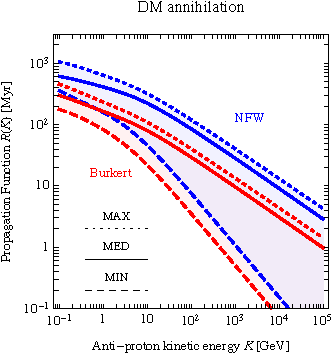
\includegraphics[width=0.4 \textwidth]{figs/PropagationFunctionAntiprotonsAnn2022}\qquad
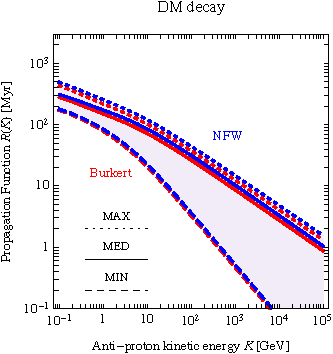
\includegraphics[width=0.4\textwidth]{figs/PropagationFunctionAntiprotonsDec2022}$$
\caption[Propagation function for $\bar p$]{\em {\bfseries Propagation functions} $\mathcal{R}(K)$ for $\bar p$ following from the propagation parameters in table~\ref{tab:proparam}
and the two DM profiles in table~\ref{fig:DMprofiles}, for DM annihilations (left) and DM decays (right). \label{fig:PropagationFunctionPbar} }
\end{figure}


\subsection{Anti-protons: practical results}
The formalism described above allows to compute the anti-proton fluxes after galactic propagation, starting from the injection fluxes detailed in section \ref{DMspectra} and depicted, e.g.,~in fig.~\ref{fig:spectraatproduction} (middle panel). 
Analogous to the treatment of electrons and positrons, it is insightful to examine qualitatively the resulting broad features of the $\bar p$ fluxes.
\begin{itemize}
\item[$\circ$] The end-point of the spectra remains at $E = M$ for DM annihilations ($E = M/2$ for DM decays). 
However, in presence of a strong re-acceleration a tail of $\bar p$ with $E >M$ may emerge. 
It should be noted that the end-point of the $\bar p$ spectra is  typically not a significant feature,  since the spectra commonly peak at $K \approx 10^{-2} M$.
\item[$\circ$] The overall normalization of the fluxes is governed by the annihilation cross section $\langle \sigma v \rangle$ (or the decay rate $\Gamma$) and is also proportional to the DM density  squared $\rho^2$ for DM annihilations ($\rho$ for DM decays).
\item[$\circ$]
 Owing to the minimal impact of energy losses and the relatively limited influence of spallations (which are confined to the thin disk), the galactic propagation of $\bar p$ typically maintains the spectral shape of the fluxes. 
 However, as commented above, the $\bar p$ spectra across different channels are rather self-similar, 
 and thus do not carry much information.
\end{itemize}
As with electrons and positrons, the injection and propagation processes introduce sources of {\bf uncertainty} in the predicted $\bar p$ fluxes. 
\begin{itemize}
\item[$\triangleright$] Galactic propagation is characterized by sets of parameters such as those in table \ref{tab:proparam}. The variation between MIN and MAX predictions is roughly independent on the $\bar p$ energy and typically does not exceed half an order of magnitude. This uncertainty was reduced considerably recently (propagation uncertainty bands of up to almost two orders of magnitudes were considered in the past), thanks to improved  determinations of the propagation parameters (see, e.g.,~\arxivref{2103.04108}{G\'enolini et al.~(2021)} in \cite{CRpropagation}, and references therein).
Solar modulation further alters  the fluxes at low energies.
\item[$\triangleright$] The uncertainty in the galactic DM distribution affects the predicted fluxes, roughly independently of energy. 
The difference between the predicted flux for a cored profile and a peaked profile is typically a factor of a few for annihilating DM, and much smaller for decaying DM. 
In addition, if DM sub-halos are present, they boost the flux in the case of DM annihilations (see section~\ref{sec:astroboost}).
\item[$\triangleright$] Uncertainties from the spallation cross section and other interactions 
are generally considered minor for the DM $\bar p$ flux and are not typically evaluated. 
However, they may be important for 
an accurate computation of the astrophysical background flux.
\end{itemize}
The limited impact of these uncertainties on the DM $\bar p$ fluxes, combined with the fact that the astrophysical background $\bar p$ spectrum is also rather well under control 
(compared, for example, to positrons) has made anti-protons a probe of choice for investigating DM and producing competitive bounds, see section \ref{sec:IDconstraints} for the current status.


\section{Anti-deuteron and heavier anti-nuclei}\label{sec:antideuterons}\index{Indirect detection!$\bar d$}
\index{Indirect detection!$\overline{\rm He}$}
The propagation of DM generated antideuterons and other light nuclei (essentially anti-helium) through the Galaxy follows closely that of anti-protons, section \ref{anti-protons}, with a few modifications~\cite{DbarHebarpropagation}. 
The transport equation remains as given in eq.~(\ref{eq:diffeqp}). 
Diffusion, dictated by the electromagnetic properties of the particles, is identical for anti-nuclei and anti-protons, with the simple substitution that the deuteron mass $m_d$ or helium mass $m_{^3{\rm He}}$, $m_{^4{\rm He}}$ must replace the proton mass in the expressions for the kinetic energy and momentum.
The convection, diffusive re-acceleration and energy loss terms are the same as those in the previous section.\footnote{
For low-$Z$ nuclei, it is customary to use the kinetic energy per nucleon, $K/n$, as a variable.
While the total kinetic energy $K$ of the particle must be used in the equations, the spectra are often presented in terms of $K/n$.}
The source term features the spectra discussed in section \ref{DMspectraDbarHe}.


\medskip

The treatment of spallations of $\bar d$ and $\overbar{\rm He}$ on interstellar gas (both `annihilating' and `non-annihilating' reactions) 
is less straightforward than for $\bar p$, largely due to the scarcity of experimental nuclear data on $\bar d$ and $\overbar {\rm He}$. The values for  $\sigma^{\rm ann}_{\bar{d}p}$, $\sigma^{\rm non-ann}_{\bar{d}p}$ and $\sigma^{\rm inel}_{\bar{d}p}$, as well as the equivalent cross sections for the $\overbar {\rm He} \, p$ processes, are required: these can be obtained experimentally from the measurements of the charge conjugated reactions induced by the $d \bar{p}$ scattering, and partially also from the $p\bar{p}$ scattering data. They can also be estimated from more general formulas derived for cosmic ray nuclei. 
Often, a good approximation is already to 
adopt simple scaling relations, such as $\sigma^{\rm inel}_{\bar{d}p} \approx 2\, \sigma^{\rm inel}_{\bar{p}p}$.


\medskip

With the ingredients described above, one can compute an anti-nucleon or anti-helium propagation function $R(K/n)$, for both annihilations and decays, in a manner analogous to the procedure followed for anti-protons. This computation can be carried out for any chosen Dark Matter (DM) galactic profile and for any set of propagation parameters listed in table~\ref{tab:proparam}. 
 It then becomes straightforward to calculate the anti-deuteron and anti-helium differential flux at Earth's location, using a formalism identical to the one in eq.~(\ref{eq:fluxpbar}).
Finally, solar modulation can be applied in a manner similar to that discussed for anti-protons, incorporating the appropriate kinematic quantities as detailed in eq.~(\ref{solarmod}). 



\section{Secondary photons}\label{sec:secondary photons}\index{Indirect detection!$\gamma$!secondary}\index{$\gamma$!secondary}
As discussed above, the galactic $e^\pm$ generated by DM in the diffusion volume of the Galaxy lose essentially all their energy into photons by means of two processes: inverse Compton scattering and synchrotron radiation. 
Bremsstrahlung radiation also plays a significant role in regions close to the galactic disk, where gas is abundant, particularly for electrons in the energy range of $\sim 1-10\,\text{GeV}$.


\smallskip

The fluxes of ICS (and bremsstrahlung) $\gamma$ rays generated in this way, as well the microwave synchrotron radiation, can thus be signatures of DM in the Milky Way. 
The same emissions can be searched for also in other systems, such as in dwarf galaxies, clusters of galaxies and even in the cosmological flux, 
provided that the necessary environmental conditions are met: the presence of ambient light for ICS (with the understanding that the CMB is always present), gas for bremsstrahlung, and a magnetic field for synchrotron emission.
Collectively, these emissions are referred to as \emph{secondary photons}, in contrast to the prompt photons discussed in section~\ref{sec:IDgamma}.

 
 \smallskip
 
The ICS flux has been investigated in great detail in recent years. One of its distinguishing features  is that it originates from `everywhere' within the diffusion volume of the galactic halo, including regions where the astrophysical background is reduced (e.g.,\ at high latitudes). 
Moreover, in areas where synchrotron energy losses are sub-dominant in comparison to ICS energy losses, the resulting ICS $\gamma$ flux is subject to only moderate astrophysical uncertainties, owing to energy conservation. 
The microwave synchrotron emission, on the other hand, is generated in significant quantities near the GC, where the intensity of the magnetic field and the density of DM are highest, resulting in greater uncertainty and more background.
However, it can also originate from large latitudes.
Finally, bremsstrahlung emission may be a relevant signature of DM under certain conditions (such as large gas density and $e^\pm$ energy $\lesssim$10 GeV).
In any case, it must be taken into account, if one aims at consistently modeling the other emissions with which it competes.

\medskip

In this section, we provide a detailed description of the computation of ICS emission (section~\ref{sec:ICS}), bremsstrahlung emission (section~\ref{sec:bremgammas}), and synchrotron radiation (section~\ref{sec:synchr}).  The methods that we describe build on the standard electro-magnetic formalism~\cite{CRtransport,CRenergylosses} and use tools in the form of {\it generalized halo functions} for ICS, bremsstrahlung and synchrotron, as  initially introduced in \cite{PPPC4DMID} and \arxivref{1505.01049}{Buch et al.~(2015)} in~\cite{CRenergylosses}. These functions, which are analogous to the halo functions used for $e^\pm$ propagation, are computed once and for all. They then enable the computation of the emission through a simple convolution with the injected electron spectrum, making the phenomenology faster to analyze for any DM model.

\subsection{Inverse Compton gamma rays}\label{sec:ICS}\index{Indirect detection!$\gamma$!inverse Compton}\index{$\gamma$!inverse Compton}
The ICS signal has its origin in the following process, alluded to earlier: energetic $e^+$ and $e^-$,  produced in the halo of the Galaxy by the annihilations or decays of DM particles, hit the low energy photons of the ambient bath (the CMB, infrared light and starlight). These collisions constitute an inverse Compton scattering, upscattering the ambient photon energy from its initial low value $E^0_\gamma$ to a final value of up to $E_\gamma \approx 4 \gamma^2 E^0_\gamma$. Here $\gamma = E_e/m_e$ is the relativistic factor of the electrons and positrons. 
As a rule of thumb, a 1 TeV electron will produce a $\sim$ 1.5 GeV soft $\gamma$-ray when scattering off the CMB ($E^0_\gamma \approx 10^{-4}$ eV), or a $\sim$ 150 GeV hard $\gamma$-ray when scattering off UV starlight ($E^0_\gamma \approx 10$ eV).

\smallskip

An accurate description of the ambient radiation field is important to compute the ICS emission in a reliable way. 
A recent appraisal of the radiation maps can be obtained from \cite{ISRFmaps}.  
It displays modifications of at most a factor of a few in the intensity of the IR and starlight fields with respect to previous determinations. 
This variation can be considered as an estimate of the astrophysical uncertainty related to the environment, affecting 
at the same time the computation of ICS energy losses and the ICS signal itself.
 It is worth mentioning, however, that these uncertainties may partly offset each other: an increase in ambient light density results in greater energy loss for the propagating $e^\pm$, leading to a suppressed $e^\pm$ spectrum, but at the same time it enhances ICS emission.
 In regions where ICS is the dominant energy-loss/emission process for the electrons and positrons, the two effects partly compensate each other.

\medskip

The differential flux of ICS photons from a
a solid angle element $d \Omega$ can be written in terms of the emissivity $j(E_\gamma,r)$ of a cell located at a distance $r\equiv|\vec x|$ from the GC as follows:
\beq
\label{eq:ICSbasic}
\frac{d\Phi_{{\rm IC}\gamma}}{dE_\gamma \, d\Omega} = \frac{1}{4\pi} \frac{1}{E_\gamma} \int_{\rm l.o.s.} ds \, j(E_\gamma,r(s,\theta)).
\eeq
For a radiative process, in general terms, the emissivity is derived as a convolution of the spatial density of the emitting medium with the power that it radiates (see e.g.~Rybicki and Lightman (1979) in \cite{CRtransport}). In this case 
\beq
\label{Rademissivity}
j(E_\gamma,r)=2\int_{m_e}^{M (/2)} \hspace{-0.45cm} dE_e\ \mathcal{P}_{\rm IC}(E_\gamma,E_e,r)\ \frac{dn_{e^\pm}}{dE_e}(r,E_e),
\eeq
where $\mathcal P=\sum_i \mathcal P_{\rm IC}^i$ is the differential power emitted into photons due to ICS radiative processes (the sum runs over the different components of the photon bath).
 The electron (or positron) number density post-diffusion and energy losses, $dn_{e^\pm}/dE_e$, has been computed in subsection \ref{sec:e+e-}. 
 (Note that this quantity was represented as $f$ in that section for simplicity, see page~\pageref{eq:diffeq}; $dn_{e^\pm}/dE_e$ 
 just corresponds to eq.~(\ref{eq:positronsfluxnox}), 
 removing the $v_{e^\pm}/4\pi$ factor.) 
The minimal and maximal electron energies in the integration limits in eq.~(\ref{Rademissivity}) are fixed by the electron mass $m_e$ and the mass of the DM particle $M$. The `$/2$' notation applies to the decay case. The overall factor of 2 before the integral 
 accounts for the fact that an equal population of positrons, in addition to electrons, is produced by DM annihilations/decays, and both contribute to the emission.


\medskip


The radiated power $\mathcal P_{\rm IC}$, using the full Klein-Nishina expression for $e\gamma$ scattering,
is (we refer the reader to \cite{CRtransport,CRenergylosses} and references therein for more details on the derivation)
\begin{equation}
\begin{split}
&\mathcal{P}_{\rm IC}^i(E_\gamma,E_e,\vec x)  =
\frac{3 \sigma_{\rm T}}{4\gamma^2}  \int_{1/4\gamma^2}^1\! dq  \left(E_\gamma-\frac{E_\gamma}{4q\gamma^2 (1-\epsilon)} \right)\times\\
&\qquad \times\frac{n_i\big(E_\gamma^0(q),\vec x \big)}{q} \left[ 2q\ln q+q+1-2q^2+\frac{1}{2}\frac{\epsilon^2}{1-\epsilon}(1-q) \right].
\end{split}
\label{eq:power}
\end{equation}
The integration variable is
\beq
\label{eq:ICSdetails}
q=\frac{\epsilon}{\Gamma_E(1-\epsilon)}, \qquad {\rm where}\qquad  \Gamma_E=\frac{4E_\gamma^0E_e}{m_e^2}\qquad \hbox{and}\qquad
\epsilon=\frac{E_\gamma}{E_e},
\eeq
and lies in the range $1/4\gamma^2\approx 0 \le q \le 1$, as expressed by the limits of the integral in eq.~(\ref{eq:power}).
Correspondingly, the energy $E_{\gamma}$ lies in the range\footnote{The combination $E_e \Gamma_E$ reproduces the `rule of thumb estimate' for $E_{\gamma}$ mentioned at the beginning of the section.} $E_\gamma^0/E_e \le E_\gamma \le E_e\, \Gamma_E/(1+\Gamma_E)$.
The non-relativistic (Thompson) limit corresponds to $\Gamma_E\ll1$, so that $\epsilon \ll 1$, and therefore the last addend in the integrand of $\mathcal P$ can be neglected. At the same time, the integration variable $q$ reduces to $y \equiv E_\gamma/(4\gamma^2 E_\gamma^0)$ with $0\le y \le 1$.
Hence, in the Thomson limit,
\beq
\mathcal{P}_{\rm IC}^i(E_\gamma,E_e,\vec x) \approx \frac{3 \sigma_{\rm T}}{4\gamma^2} E_\gamma  \int_{0}^1 \hspace{-0.2cm} dy   \frac{n_i\big(E_\gamma^0(y),\vec x \big)}{y} \left[ 2y\ln y+y+1-2y^2 \right]\qquad {\rm [Thomson\ limit]}.
\label{eq:powerThomson}
\eeq
By substituting 
 $\mathcal{P}_{\rm IC}$ and $n_{e^\pm}$ in eq.~(\ref{Rademissivity}), 
 the IC differential flux can be recast in a more convenient form:
\beq
\frac{d\Phi_{{\rm IC}\gamma}}{dE_\gamma\, d\Omega} = \frac1{E_\gamma^2}\frac{r_\odot}{4\pi} 
\left\{\begin{array}{ll}
\displaystyle \frac12 \left(\frac{\rho_\odot}{M }\right)^2 \int_{m_e}^{M } \hspace{-0.35cm} dE_{\rm s}  \ \langle \sigma v \rangle_{\rm tot} \frac{dN_{e^\pm}}{dE}(E_{\rm s})  \ I_{\rm IC}(E_\gamma,E_{\rm s},b,\ell) & {\rm (annihilation),} \\[5mm]
\displaystyle \frac{\rho_\odot}{M } \int_{m_e}^{M /2}\hspace{-0.60cm} dE_{\rm s} \ \Gamma_{\rm tot}  \frac{dN_{e^\pm}}{dE}(E_{\rm s})  \ I_{\rm IC}(E_\gamma,E_{\rm s},b,\ell) &{\rm (decay),}
\end{array}\right.
\label{eq:summaryIC}
\eeq
where $E_{\rm s}$ is the $e^\pm$ injection energy and $I_{\rm IC}(E_\gamma,E_{\rm s},b,\ell)$ (which has the dimensionality of an energy) is a halo function for the IC radiative process. 
Thus this formalism permits to express the flux of ICS $\gamma$ in terms of the convolution of the electron injection spectrum $dN_{e^\pm}/dE$ and the appropriate halo functions, in close analogy with the formalism for charged particles.
Explicitly, we can write $I_{\rm IC}$ in terms of the ICS ingredients discussed above and the generalized halo functions for $e^\pm$  introduced in section~\ref{sec:epemhalofunctions}:
\beq\label{HaloICS}
I_{\rm IC}(E_\gamma,E_{\rm s},b,\ell)= 2\, E_\gamma \int_{\rm l.o.s.} \frac{ds}{r_\odot} \left( \frac{\rho(r(s,\theta))}{\rho_\odot} \right)^p \hspace{-0.2cm} \int_{m_e}^{E_{\rm s}}\hspace{-0.3cm}dE\,  \frac{{\sum_i \mathcal P_{\rm IC}^i(E_\gamma,E,r(s,\theta))}}{b_{e^\pm}(E,r(s,\theta))}\,  I(E,E_{\rm s},r(s,\theta)),
\eeq
where $p=1 (2)$  for DM decay (annihilation). 
The intensity of the interstellar radiation, $\sum_i n_i$, cancels out in the ratio  $\sum_i \mathcal{P}_i/b_{e^\pm}$, up to the sub-leading synchrotron contribution.
The final step in obtaining the differential ICS $\gamma$ flux $d\Phi_{\rm IC \gamma}/dE_\gamma d\Omega$ consists of performing the convolution integral over $E_{\rm s}$ in eq.~(\ref{eq:summaryIC}) for a particular DM generated prompt $e^\pm$ energy spectrum.  

The differential flux from a region $\Delta \Omega$ is obtained by integrating over the galactic polar coordinates
$b$ and $\ell$, defined in eq.\eq{galcoord}, 
\beq
\frac{d\Phi_{\rm IC \gamma}}{dE_\gamma} = \iint db\, d\ell\, \cos b\, \frac{d\Phi_{\rm IC \gamma}}{d\Omega\, dE_\gamma}.
\label{eq:summaryICI}
\eeq
Due to the intertwined dependence of the halo functions on $b$ and $\ell$ and on $E_\gamma$ and $E_s$, the geometrical integral cannot be factored out as in the case of prompt $\gamma$ rays. 
Consequently, a simple definition of the $\bar J$  factor is not possible.



\medskip

We should emphasize that the halo function formalism is specific to the galactic signal. 
For other systems, or for more complex analyses,  the ICS signal can be computed directly using the ingredients in eq.s~(\ref{eq:ICSbasic})$-$(\ref{eq:ICSdetails}).



\subsection{Bremsstrahlung gamma rays}\index{Indirect detection!$\gamma$!bremsstrahlung}\index{$\gamma$!bremsstrahlung}
\label{sec:bremgammas}

The bremsstrahlung signal is generated by energetic electrons and positrons, produced in the galactic halo by the annihilations or decays of DM particles. The $e^\pm$ interact with the electromagnetic field of the atoms constituting interstellar gas, emitting a bremsstrahlung photon. The energy of the emitted photon peaks  at a fraction of the initial energy of the $e^\pm$, typically between 1/10 and 1/2, depending on  both the $e^\pm$ spectrum and on local conditions. 
Notably, this process becomes the dominant channel for energy loss of $e^\pm$ in the energy range of $1-10$ GeV, particularly in regions where the density of interstellar gas is sizeable.


For an accurate assessment of the bremsstrahlung signal, one requires maps of the gas distribution and composition within the Galaxy, which are only partially available~\cite{gasmaps}.
On large scales, coarse-grained maps for the density of hydrogen (in atomic, molecular and ionized form) as well as atomic helium are available: they show an average density of $\mathcal{O}(1)$ particles/cm$^3$
in the galactic disk, rapidly decreasing in the vertical direction, e.g., to $\mathcal{O}(0.01)$ atoms/cm$^3$ at 1 kpc above the galactic plane.
The gas density in the Galaxy's central regions is expected to be substantially higher, possibly reaching $\mathcal{O}(100)$ particles/cm$^3$ within the inner 200 pc around the Galactic Center (the so-called Central Molecular Zone), or even higher in the inner few parsecs, where accretion occurs on the central black hole.  
These variations in density introduce significant astrophysical uncertainties in the computation of the DM bremsstrahlung signal. However, analogous to the ICS case, these uncertainties are partially mitigated by the conservation of energy. A higher gas density results in increased energy loss for propagating $e^\pm$, leading to a suppressed spectrum but simultaneously enhancing bremsstrahlung emission. In regions where bremsstrahlung dominates as the energy-loss/emission process for $e^\pm$, these two effects largely compensate each other.


\medskip

The computation of the bremsstrahlung emission and its generalized halo functions follows quite closely the computation for ICS in the previous subsection. 
For completeness, we briefly summarize the essential components here. In exact analogy with eq.~(\ref{eq:summaryIC}), the bremsstrahlung differential flux can be written as: 
\beq
\frac{d\Phi_{{\rm brem}\gamma}}{dE_\gamma\, d\Omega} = \frac1{E_\gamma^2}\frac{r_\odot}{4\pi} 
\left\{\begin{array}{ll}
\displaystyle \frac12 \left(\frac{\rho_\odot}{M }\right)^2 \int_{m_e}^{M } \hspace{-0.35cm} dE_{\rm s}\ \langle \sigma v \rangle_{\rm tot} \frac{dN_{e^\pm}}{dE}(E_{\rm s})  \ I_{\rm brem}(E_\gamma,E_{\rm s},b,\ell) & {\rm (annihilation),} \\[5mm]
\displaystyle \frac{\rho_\odot}{M } \int_{m_e}^{M /2}\hspace{-0.60cm} dE_{\rm s}\  \Gamma_{\rm tot}  \frac{dN_{e^\pm}}{dE}(E_{\rm s})  \ I_{\rm brem}(E_\gamma,E_{\rm s},b,\ell)  &{\rm (decay),}
\end{array}\right.
\label{eq:summarbrem}
\eeq
where now (in analogy with eq.~(\ref{HaloICS})) the generalized halo function for bremsstrahlung is
\beq\label{Halobrem}
I_{\rm brem}(E_\gamma,E_{\rm s},b,\ell)= 2\, E_\gamma \int_{\rm l.o.s.} \frac{ds}{r_\odot} \left( \frac{\rho(r(s,\theta))}{\rho_\odot} \right)^p  \int_{m_e}^{E_{\rm s}}\hspace{-0.3cm}dE\,  \frac{{\mathcal P_{\rm brem}(E_\gamma,E,r(s,\theta))}}{b_{e^\pm}(E,r(s,\theta))}\,  I(E,E_{\rm s},r(s,\theta)),
\eeq
where as before $p=1(2)$  for DM decays (annihilations), and $I$ is the $e^\pm$ generalized halo function.
The bremsstrahlung power is
\begin{equation}
\label{eq:Pbrem}
{\mathcal P}_{\rm brem} (E_\gamma, E, \vec{x}) = c \, E_\gamma \sum_i n_i(\vec{x}) \frac{d \sigma_i(E_\gamma,E)}{dE_\gamma},
\end{equation}
where $n_i$ are the number densities of the gas species and the differential bremsstrahlung cross section is given by
\begin{equation}
\label{eq:sigma}
\frac{{\rm d} \sigma_i(E_{e^\pm},E_\gamma)}{{\rm d} E_\gamma}=\frac{3\,\alpha\sigma_{\rm T}}{8\pi\,E_\gamma}\left\{\left[1+\left(1-\frac{E_\gamma}{E_{e^\pm}}\right)^2\right]\phi^i_1-\frac{2}{3}\left(1-\frac{E_\gamma}{E_{e^\pm}}\right)\phi^i_2\right\}\,.
\end{equation}
Here, $\phi^i_{1,2}$ are scattering functions, which depend on the properties of the scattering system: ionized, atomic or molecular, hydrogen or helium. We direct the reader to the relevant literature for their explicit forms (see, e.g.,~\arxivref{1505.01049}{Buch et al.~(2015)} in~\cite{CRenergylosses} for a recapitulation and references).

\medskip

We stress again that the halo function formalism is specific to the galactic signal. For other systems, or for more complex analyses, the bremsstrahlung signal can be computed
directly using the power in eq.~(\ref{eq:Pbrem}), in conjunction with the equivalent of the general expressions in eq.s~(\ref{eq:ICSbasic})$-$(\ref{Rademissivity}).

\subsection{Synchrotron radio waves}\index{Indirect detection!synchrotron}\index{$\gamma$!synchrotron}
\label{sec:synchr}

Radio waves are produced by the DM generated high-energy electrons and positrons, via the synchrotron process, as they gyrate in the galactic magnetic field. 
As a rule of thumb, an electron or positron with momentum $p$ moving in a turbulent magnetic field of intensity $B$ generates radio waves that peak at frequency $\nu \approx 3 e B p^2/4\pi m_e^3 \approx 4.2 \ {\rm Hz}\, (B/\mu {\rm G}) (p/m_e)^2$. 
For example, an electron with energy 1 GeV (10 GeV) in a 5 $\mu$G magnetic field, which is typical of the local galactic environment, would emit radio waves at 80 MHz (8 GHz).
Radio maps of the Milky Way, with varying degrees of coverage and completeness, are available between 22 MHz and 2.3 GHz. In addition, {\sc Planck-Lfi} microwave maps cover up to 70 GHz~\cite{Planckresults}.


The synchrotron signal depends on the intensity of the magnetic field, whose uncertainties we have already briefly discussed on page \pageref{Bgalactic}. 
For signals that originate very close to the GC, the impact can be sizable, since in that region the magnetic field is highly uncertain (see, e.g.,~\arxivref{0811.3744}{Bertone et al.~(2009)} in \cite{DMradiobounds}).  
In contrast, for signals from the galactic halo, the resulting uncertainty in the radio emission was found to be minimal (see, e.g.,~\arxivref{1505.01049}{Buch et al.~(2015)} in~\cite{CRenergylosses}).


\medskip

The synchrotron power (in erg s$^{-1}$ Hz$^{-1}$), emitted by an isotropic distribution of relativistic electrons with energy $E_e$ 
in a uniform magnetic field $B$, is given by
\begin{equation}
\mathcal{P}_{\rm syn}(\nu,E_e,\alpha)=\sqrt{3}\, \frac{e^3 \, B \sin\alpha}{m_e\, c^2} F(x),
\label{eq:syncreg}
\end{equation}
where
\beq x= \frac{\nu}{\nu_c'}, \qquad  \nu_c'=\frac{\nu_c }{2} \sin \alpha, \qquad\nu_c = \frac{3}{2 \pi}\frac{e}{m_ec} B\gamma^2.\eeq
Here,  $\alpha$ is the angle between the line of sight and the magnetic field direction, and $\gamma = E_e/m_e$ is the Lorentz factor of the electron or positron.
The synchrotron kernel $F(x)$ is defined as
$$ F(x)=x \int_x^{\infty} K_{5/3}(x^{\prime}) dx^{\prime},$$
where $K_{n}$ is the modified Bessel function of the second kind of order $n$.
When the magnetic field is randomly oriented, as is the case in the galaxy, the synchrotron power must be averaged over the pitch angle $\alpha$, leading to
\begin{equation}
\mathcal{P}_{\rm syn}(\nu,E_e)=\frac{1}{2}\int_0^{\pi} d\alpha \, \sin(\alpha) \, \mathcal{P}_{\rm syn}(\nu,E,\alpha) \, .
\label{eq:syncran}
\end{equation}
For relativistic electrons ($\gamma \circa{>} 2$) 
one obtains (see, e.g.,~Ghisellini et al.~(1988) in \cite{CRenergylosses})
\begin{equation}
\mathcal{P}_{\rm syn}(\nu,E)=2\sqrt{3} \, \frac{e^3\, B}{m_ec^2} y^2 \left[ K_{4/3}(y) K_{1/3}(y)-\frac{3}{5}y\Big( K_{4/3}(y)^2-K_{1/3}(y)^2\Big)\right],
\label{eq:sync1}
\end{equation}
with $y=\nu/\nu_c$.
Integrating this expression over $\nu$ yields the total power emitted by an electron of energy $E$ across all frequencies, i.e., eq.~(\ref{eq:b(E)}) (synchrotron portion).
The synchrotron emissivity $j_{\rm syn}(\nu,r)$ is then computed using the equivalent of the general expression in eq.~(\ref{Rademissivity}).


\medskip

Finally, the observable of interest for comparison with observational data is the intensity 
$\mathscr{I}$ 
of the synchrotron emission (in erg cm$^{-2}$ s$^{-1}$ Hz$^{-1}$ sr$^{-1}$) from a certain direction of observation. It is obtained by integrating the emissivity along the line-of-sight. Schematically, 
\begin{equation}
\mathscr{I}(\nu,b,\ell) = \frac{1}{4\pi}  \int_{\rm l.o.s.}ds \,  j_{\rm syn}(\nu,r,z),
\label{eq:sync3}
\end{equation}
where the point in $(r,z)$ is identified by the parameter $s$ along the line of observation, characterized by the galactic latitude $b$ and longitude $\ell$: $r(s,b,\ell), z(s,b,\ell)$.
\medskip




Collecting the above expressions (equations (\ref{eq:sync3}) and the equivalent of (\ref{Rademissivity}), with (\ref{eq:sync1}) and the generalized version of (\ref{eq:positronsfluxnox})), the synchrotron intensity $\mathscr{I}$, at a fixed frequency $\nu$ and at galactic coordinates $(b,\ell)$, is given by 
\begin{equation}
 \mathscr{I}(\nu,b,\ell)=\frac{r_\odot}{4\pi} \left\{
 \begin{array}{ll}
 \displaystyle\!\!
 \frac{1}{2}\left(\frac{\rho_{\odot}}{M }\right)^2  \int_{m_e}^{M } \hspace{-0.35cm} dE_s \  \langle \sigma v \rangle_{\rm tot} \frac{dN_{e^{\pm}}}{dE}(E_s)\ I_{\rm syn}(\nu,E_s,b,\ell) & {\rm (DM annihilation),}\\
\displaystyle\!\!
 \left(\frac{\rho_{\odot}}{M }\right) \int_{m_e}^{M /2} \hspace{-0.60cm} dE_s \  \Gamma_{\rm tot} \frac{dN_{e^{\pm}}}{dE}(E_s)\ I_{\rm syn}(\nu,E_s,b,\ell) & {\rm (DM decay),}
 \end{array}
 \right.
\label{eq:synchalof}
\end{equation}
with the {\it generalized synchrotron halo function} $I_{\rm syn}(\nu,E_s,b,\ell)$ defined as
\begin{equation}
I_{\rm syn}(\nu,E_s,b,\ell)= \int_{\rm l.o.s.}\frac{ds}{r_\odot} \left(\frac{\rho(r,z)}{\rho_\odot}\right)^p \  2 \int_{m_e}^{E_s} dE  \frac{\mathcal{P}_{\rm syn}(\nu,E)}{b_{e^\pm}(E,r,z)} \ I(E,E_s,r,z),
\label{eq:synchalof2}
\end{equation}
in terms of $I$, the generalized halo function for $e^\pm$. 
Here, $p = 1 (2)$ for the DM decays (annihilations), and, again, $r, z$, are to be written in terms of galactic
coordinates $s,\ell,b$.

For completeness, we mention that the synchrotron intensity $\mathscr{I}$ is often traded for the {\em brightness temperature} $T(\nu)$, \index{Synchrotron brightness temperature} expressed in Kelvin, which is just the temperature that a black body would have to possess in order to emit the same intensity at a given frequency. One has~\footnote{Here we take $k_B = c = 1$, where $k_B$ the Boltzmann constant.}
\begin{equation}
 T(\nu)=\frac{\mathscr{I}(\nu)}{2\, \nu^2} .
\label{eq:syncT}
\end{equation}

\medskip


Once again, we emphasize that the halo function formalism is specific to the galactic signal. For other systems, or when performing more complex analyses, the synchrotron signal can be computed by directly utilizing the power expression in eq.~\eqref{eq:sync1}, along with the generic definitions provided in eq.s~\eqref{Rademissivity} and \eqref{eq:sync3}.





\section{Enhancements}\label{sec:boost}

The indirect detection signals
can be enhanced by a number of 
different mechanisms. In this section, we discuss the boost caused by clumps in the DM distribution (section~\ref{sec:astroboost}) and the enhancements 
that depend on the micro-physics of the annihilation process (section~\ref{sec:sommerfeld}). 
These enhancements typically arise only for annihilating DM, whereas in scenarios involving decaying DM, such enhancements are absent.




\subsection{Boost due to DM sub-halos}\label{sec:astroboost}\index{Boost factor}\index{Indirect detection!boost factor}\index{Sub-halos!boost factor}
In the preceding subsections, we assumed that the cosmic and galactic DM distribution was smooth. 
However, one of the main results of the clustering history is the emergence of a hierarchical structure 
comprising halos and sub-halos of various sizes throughout the cosmos. 
This structure gives rise, a fortiori,  to the presence of small DM sub-halos within the larger halos of galaxies.
The expected number distribution of these sub-structures as a function of their mass was discussed in section~\ref{sec:haloMf}. 


Small-scale inhomogeneities typically enhance the indirect detection signals of DM annihilations, 
since these signals are proportional to $\med{\rho^2}>\med{\rho}^2$~\cite{BoostFactorID}. 
The position of the DM sub-halos within the galaxy and the cosmos is generally unknown, so that the enhancement
is usually taken into account by an overall multiplicative number known as the {\em boost factor} $B \sim \med{\rho^2}/\med{\rho}^2$, by which the signal from a smooth DM distribution should be multiplied. 
In a simplified scenario where DM is uniformly distributed within a volume $V$ and becomes concentrated within a sub-volume $V' < V$, this means that 
$B = V/V'$.



\medskip
In principle, the computation of the boost factor $B$ follows in a straightforward manner from the mass function formalism discussed in section~\ref{sec:haloMf}. Using 
the predicted number $n$ of subhalos per mass $\Mcal$, $dn/d\Mcal$, 
one can include the annihilation signal from each subhalo by integrating over this halo mass distribution, yielding the total signal contributed by substructures. Explicitly, we have
\beq
\label{eq:boostnaif}
B \propto \int_{\Mcal_{\rm min}} d\Mcal \frac{dn}{d\Mcal} \int dr \ 4 \pi r^2 \rho^2_{\rm sub}(r,\Mcal),
\eeq
where $\rho_{\rm sub}(r,\Mcal)$ is the density profile of a sub-halo of mass $\Mcal$ and the coordinate $r$ refers to the center of the subhalo. 
For DM density $\rho_{\rm sub}$ we can use one of the forms  discussed in section \ref{rho(r)} for the Galaxy, if one assumes, as it is often done, that the subhalos are `small-size reproductions' of the main halo. 
However, numerical simulations often reveal that subhalos possess higher DM densities in their inner regions and are, on average, more concentrated than `normal' halos of the same mass.
Therefore, more peaked $\rho_{\text{{sub}}}$ profiles are sometimes used.  
In eq.~(\ref{eq:boostnaif}), the integral over the volume of the subhalo is truncated at a specific radius  (typically its virial radius). 
The integral over the halo masses, in turn, is cut from below at $\Mcal_{\rm min}$, the minimal mass of the sub-halos (which depends on the microscopic properties of the DM particle as discussed in section~\ref{sec:haloMf}).
It is noteworthy that the integral is primarily dominated by small halo masses.

\smallskip



However, detailed studies have revealed that the situation is more complex, especially regarding galactic DM signals~\cite{BoostFactorID2}.
First, the halo mass function $dn/d\Mcal$ 
gets modified during the late stages of galactic evolution.
 Specifically, sub-halos can be tidally stripped by the gravitational influence of the host halo and other sub-halos, leading to their dissolution.
 This phenomenon particularly affects small halos, modifying the value of the 
 minimal halo mass.
Additionally, sub-halos can be loosened and subsequently dissolved when crossing the galactic disk due to gravitational interactions, an effect referred to as {\em `disk shocking.' }
Encounters with individual stars have also been shown to potentially impact these structures.
Cosmological simulations (including baryons) have been used to model the above effects and to compute more realistic boost factors, although the challenge of  fully matching the simulated galaxies to the real Milky Way remains. 
Analytical approaches have been used as well, but they often struggle to capture the full complexity of these processes and often have to adopt simplifying assumptions. 
In general terms, these gravitational effects are more pronounced in the central regions of the Galaxy, which is thus more severely depleted of subhalos, while the outskirts remain populated. 
Consequently, the boost factor for $\gamma$-rays from the GC areas is expected to be minimal.
That is, in general the boost factor depends on the observed/sampled area, and is not simply a common overall factor. 

\smallskip

Finally, the effective boost factor of the signals detected at Earth depends both on the nature and the energy of the cosmic ray species, i.e.,~whether one considers $\gamma$-rays (or neutrinos), electrons/positrons or anti-protons/anti-nuclei. This dependence arises because the signal collected at Earth  is sensitive to the source volume, as mentioned in the respective sections~\ref{sec:IDgammaMW}, \ref{sec:e+e-} and \ref{anti-protons}, and this volume, in turn,  depends on the particle energy. For instance, the boost factor is higher for high-energy positrons than for low-energy ones: low-energy $e^+$ originate from a large volume encompassing regions towards the GC, where the smooth DM density is high, 
and therefore the weight of the subhalos is comparatively lower. 
Conversely,  the boost factor is higher for low-energy anti-protons than for high-energy ones: low-energy $\bar p$ are more affected by convection and the (subdominant) energy losses and therefore come from a smaller, more local volume, where the component of the signal due to subhalos is comparatively higher than that from the smooth component. 
As a result, one should consider a variety
of energy-dependent boost factors $B_i(E)$, for each species $i$. However, these variations are globally mild and thus the approximation of using a single unified boost factor $B$ remains widely used in practice. 

\medskip

The predictions 
for the boost factor(s) 
have varied over the years.
Initial works estimated very high values, often in the hundreds or thousands. 
Values as high as $B \approx 10^9$ have even been suggested. 
More detailed recent analyses found that boost factors do not exceed $B \sim \mathcal{O}(10)$. 
The boosts for $e^\pm$ and $\bar p$ are found to reach at most $B \approx 30$ (at high and low energy respectively, and in extremal configurations). 
The boost factors for $\gamma$-rays, while dependent on the abundance of clumps in the observed region as previously discussed, have been found to be similar in magnitude.
It is worth noting that non-standard cosmologies, featuring enhanced small-scale primordial fluctuations, phase transitions, or topological defects, may give rise to more DM clumps and consequently larger boost factors. These concepts are further explored in section~\ref{sec:PBHform} in the context of BH formation.





\subsection{Sommerfeld and bound-state enhancement}\label{sec:sommerfeld}
\index{Sommerfeld corrections!indirect detection}\index{Indirect detection!Sommerfeld}\index{DM properties!bound state}
\index{Indirect detection!bound states}\index{Bound state!indirect detection}

In models where an attractive force among two DM particles is mediated by a boson (for example the $W,Z$ vectors, or some dark photon)
with mass $M_V$ and coupling  $\alpha_g =g^2/4\pi $ to DM,
the cross section of DM annihilations is enhanced in the relevant non-relativistic limit, $ v_{\rm rel}\ll 1$~\cite{Sommerfeld}.
This Sommerfeld enhancement was discussed in section~\ref{Sommerfeld} and is estimated as 
\beq S \sim \max \left(1, \frac{v_{\rm max}}{\max ( v_{\rm rel}, v_{\rm min})} \right),
\eeq
 where
$v_{\rm max} =\pi\alpha_g$ and $ v_{\rm min} =M_V/M $.
The Sommerfeld effect enhances both
the cross section for cosmological thermal freeze-out 
(with relative DM velocity $v_{\rm rel}^{\rm cosmo} \sim 1/\sqrt{25}$, see below eq.\eq{DMrelicmassTeV})
as well as the cross section for indirect detection ($v_{\rm rel}^{\rm MW}\sim 10^{-3}$ in the Milky Way).
 Consequently, in DM models where the Sommerfeld effect is present, and assuming thermal freeze-out, the DM annihilation cross-section relevant for indirect detection in Milky Way can be enhanced by a factor of up to $\sim v_{\rm rel}^{\rm cosmo}/v_{\rm rel}^{\rm MW} \sim 200$ compared to its 'standard' value given in eq.\eq{sigmavcosmo}.
Indirect signals from DM annihilations in dwarf galaxies may receive even greater enhancements, as $v_{\rm rel}$ is smaller,
especially in the smallest dwarfs (see~\cite{1702.00408}).

\smallskip

The Sommerfeld effect is accompanied by bound-state effects, 
which can lead to larger resonant enhancements at specific DM velocities. 
Such enhancements occur when the collision energy equals the mass of a particular bound state.
This same effect can arise in models where DM is accompanied by extra particles that can be resonantly produced
in DM DM annihilations.




\section{Neutrinos from the Sun}\index{Indirect detection!$\nu$!from the Sun}\index{Neutrino!from the Sun}\index{Sun!$\nu$}
\label{sec:DMnu}
The DM particles in the halo of the Milky Way have a small, yet finite, probability of scattering with a nucleus of a massive celestial body, such as the Sun or the Earth, if their orbit intersects with it.
If the DM particles' velocity after scattering is less than the escape velocity from that body, they become gravitationally bound and begin to orbit around it.
Upon additional scatterings, they eventually sink into the center of the body and accumulate, building up a local DM over-density concentrated in a relatively small volume. 
In this dense region, the DM particles can annihilate into Standard Model particles, leading to the production of energetic neutrinos.
The neutrinos, after undergoing oscillations and interactions within the dense matter of the astrophysical body, are the only species that can escape.
A detection of high-energy neutrinos from the center of the Sun or the Earth
(on top of the lower-energy neutrino backgrounds due to nuclear fusion and radioactive processes)
would thus constitute a signal of DM~\cite{DMnu}. 


\smallskip

The expected differential neutrino flux is:
\begin{equation}
\frac{d\Phi_\nu}{dE_\nu} = \frac{\Gamma_{\rm ann}}{4\pi d^2} \, \frac{dN_\nu}{dE_\nu},
\label{eq:nuflux}
\end{equation}
where $d$ is the distance of the neutrino source from the
detector (either the Sun--Earth distance $r_{\rm SE}$ or the Earth radius $R_\oplus$),
$dN_\nu/dE_\nu$ is the neutrino flux produced per DM annihilation after taking into account neutrino propagation effects
(oscillations and absorption), and $\Gamma_{\rm ann}$ is the DM annihilation rate.
The latest results from {\sc IceCube} and {\sc Antares} (see section \ref{sec:DMnustatus}) 
set bounds on the latter, at levels ranging from $10^{20}$ to $10^{23}$ annihilations$/{\rm sec}$, depending on the DM mass and annihilation channel. 
These bounds can be translated into constraints on the capture rate of DM particles inside the celestial body and therefore on the DM scattering cross sections on nuclei, as discussed below. 
Neutrinos emanating from the centers of the massive celestial bodies 
serve as an illustrative example of a DM search strategy that employs the tools of indirect detection to probe the physical quantities involved in standard direct detection.


\medskip


More involved scenarios can also be considered \cite{NSDMnu}. For instance, \arxivref{1702.02768}{Garani and Palomares-Ruiz (2017)} and \arxivref{2308.12336}{Maity et al. (2023)} considered the case in which DM scatters on electrons rather than nuclei. \arxivref{0907.3448}{Zentner (2009)} investigated the case in which DM also possesses `self-interactions', leading to enhanced capture rate. {\sc Icecube} derived bounds on this scenario (\arxivref{1312.0797}{Albuquerque et al.~(2014)}). 
Additional scenarios are discussed in section~\ref{sec:DMnuother}.

In the rest of this section, 
we restrict our attention to the conventionally considered case of WIMP-like DM particles accumulating and annihilating into Standard Model neutrinos in the center of a celestial body.
Our focus will primarily be on the Sun, as the signals from the Earth are not promising for this standard scenario.


\medskip

 \subsubsection{Solar atmospheric neutrinos as a background}

An irreducible background to the high energy neutrinos from DM annihilations in the center of the Sun comes from neutrinos produced by cosmic ray interactions within the solar corona~\cite{SAnu}.
This phenomenon is analogous to the creation of the familiar `atmospheric neutrinos', but occurs in the `atmosphere' of the Sun rather than the Earth.
  When computing this effect, neutrino oscillations must be taken into account. The spectrum of these solar atmospheric neutrinos is harder than the corresponding terrestrial one due to the lower gas densities in the corona, which cause less energy loss for the showering particles, and due to the influence of the intense solar magnetic field.
This background is effectively irreducible, as the angular resolution of current neutrino experiments is insufficient to distinguish between the neutrinos produced across the entire surface of the Sun and those originating from the center where DM annihilations occur.
According to the latest recalculations, this background is only a factor of 10 below the current sensitivity of the experiments. 



\subsection{Computation of the DM annihilation and capture rates}\label{sec:captureDMsun}\index{DM capture}
To begin with, let's consider 
DM after capture. 
Repeated scatterings thermalise DM particles to the temperature at the center of the Sun, $T_\circledast=15.5~10^6\,{\rm K}$, \label{Tsuncore} 
such that the DM density acquires a spherically symmetric Boltzmann form, 
$n(r) \propto \exp[-M\, \phi(r)/T_\circledast] $, 
where $\phi(r) = \int_0^r dr \, G M(r)/r^2$ is the Newton potential inside the Sun, written in terms of the solar mass $M(r)$ enclosed within a sphere of radius $r$. 
Taking for simplicity the matter density in this volume to be constant 
and equal to the central density of solar matter, 
$\rho_\circledast=151\,{\rm g}/{\rm cm}^3$, all integrals can be explicitly evaluated. 
One finds  $\phi(r) -\phi(0)= 2\pi G\rho_\circledast r^2/3$, so that the 
DM particles are concentrated within a small region around the center of the Sun,
\beq\label{eq:n(r)}
n(r) \propto e^{-r^2/r_{\rm DM}^2} \quad {\rm with} \qquad  
r_{\rm DM} = \left(\frac{3 T_\circledast}{2 \pi \, G \rho_\circledast \, M} \right)^{1/2}\approx
0.01 \, R_\circledast \sqrt{\frac{100 \, {\rm GeV}}{M}},
\eeq
where $R_\circledast \approx 7~10^8\,{\rm m}$ is the radius of the 
Sun.\footnote{The size of the thermal sphere of DM can also be estimated using the virial theorem, obtaining a similar result.
The average kinetic energy of the thermalized DM is $\langle K \rangle = \frac32 T_\circledast$. The average potential energy of a DM particle of mass $M$ located at the outer shell is $\langle V \rangle = - G \, M(r_{\rm DM}) \, M / r_{\rm DM}$ with $M(r_{\rm DM})= \frac43 \pi r_{\rm DM}^3 \, \rho_\circledast$, assuming that the DM density is subdominant with respect to the solar matter density. Corrections are necessary when this no longer holds or if DM starts self-gravitating: this does not happen in the Sun, but is conceivable in other astrophysical bodies (see section \ref{sec:CaptureStars}). 
The virial theorem $\langle K \rangle = - \frac12 \langle V \rangle$ gives $r_{\rm DM} = \left(\sfrac{9T}{4\pi \, G \rho_\circledast M}\right)^{1/2}$.}
Similar expressions hold for other astrophysical bodies, after adapting appropriately the $_\circledast$ quantities.\footnote{In this section and throughout this chapter, we use the subscript $_\circledast$ to indicate quantities related to the Sun, differentiating them from those labeled with $_\odot$. For example, $\rho_\circledast$ refers to the Sun's central density, while $\rho_\odot$ is the DM density at the Sun's position in the Galaxy.}


\smallskip


Next, we turn our attention to the calculation of
 the number $N$ of DM particles captured inside the Sun.
This varies with time as
\beq \frac{dN}{dt} = \Gamma_{\rm capt}- \Gamma_{\rm evap} -2\Gamma_{\rm ann},
\label{eq:DMcaptured}
\eeq
where: 
\begin{itemize}
\item[$\triangleright$] $\Gamma_{\rm capt}$ is the capture rate discussed below; it does not depend on $N$.
\item[$\triangleright$] $\Gamma_{\rm evap}$ is the DM evaporation rate proportional to $N$; it is negligible in the Sun unless DM is lighter than $M \circa{<} T_\circledast/v_{\rm esc}\sim\GeV$\label{vescSun}.
\item[$\triangleright$] $\Gamma_{\rm ann}$ is the DM annihilation rate; it is proportional to $N^2$. 
Since 2 DM particles participate in annihilation, the annihilation rate appears multiplied by 2 in \eqref{eq:DMcaptured}.
It is given by an equation similar to eq.\eq{gamma:ann},
\beq 
2\Gamma_{\rm ann} = 
\int dV \, n^2(\vec x)\, \langle \sigma v \rangle = C_{\rm ann} \, N^2,
\eeq
where $n(\vec x)$ is the number density of DM particles at position $\vec x$ inside the Sun, 
such that the total number of DM particles is $N=\int dV\, n$.
Using the DM density distribution in eq.\eq{n(r)} gives
$C_{\rm ann} \sim \langle\sigma v\rangle/r_{\rm DM}^3$ or, more precisely,
\beq \label{eq:C_A}
C_{\rm ann}=\langle\sigma v\rangle \left(\frac{G M \rho_\circledast}{3T_\circledast}\right)^{3/2}.
\eeq
\end{itemize}
Neglecting $\Gamma_{\rm evap}$ and then solving the first order differential equation\eq{DMcaptured} 
gives
\beq 
\label{eq:Gamma:ann:solution}
\Gamma_{\rm ann} = \frac{\Gamma_{\rm capt}}{2} \tanh^2 \left(\frac{t}{\tau}\right) \simeq \frac{\Gamma_{\rm capt}}{2},
\eeq
where $\tau = 1/\sqrt{\Gamma_{\rm capt} C_{\rm ann}}$ is the characteristic time-scale set by the competing processes of capture and annihilation. The last equality in \eqref{eq:Gamma:ann:solution} holds when the elapsed time is large enough compared to $\tau$ so that one can approximate $\tanh(t/\tau)\approx 1$. 
This is typically achieved for the Sun, but not for the Earth. 
Physically, this means that the fast (compared to the age of the Sun) processes of capture and annihilation come to an equilibrium: any additional captured particles thermalize and eventually annihilate away.
In this case, the annihilation rate $\Gamma_{\rm ann}$ is 
determined entirely by the capture rate $\Gamma_{\rm capt}$, which acts as the bottleneck. 


\subsubsection{The DM capture rate}
We can distinguish two regimes for
the capture rate of DM by a macroscopic celestial body (the body has radius $R$ and contains $N_N$ matter particles (e.g.,~hydrogen nuclei) with mass $m_N$):
\begin{enumerate}
\item The capture rate is of geometric size, if  the DM/matter cross section is large enough, $\sigma_N \gg \sigma_*  \approx \pi R^2/N_N$,
so that every DM particle that hits the body also gets captured,
\beq \label{eq:GammaCaptGeom}
\Gamma_{\rm capt} =  \frac{\rho_{\rm DM}}{M}
\langle v_{\rm rel}\rangle \pi R^2 \approx \frac{1.3~10^{26}}{\rm sec} \frac{\rho_{\rm DM}}{0.3 \, \sfrac{\rm GeV}{\rm cm^3}} \frac{\TeV}{M} 
 \frac{\langle v_{\rm rel}\rangle}{10^{-3}} \frac{R^2}{R_{\circledast}^2},
 \eeq
where $\rho_{\rm DM}/M$ is the  number density of DM particles at the location of the body. 
In the case of the Sun, $\sigma_* \sim 10^{-35}\cm^2$.
Such a 
large scattering cross section 
is experimentally excluded, as mentioned above. 

\item If 
DM particle has only a small probability of interacting with the body, the capture rate is estimated as
\beq 
\Gamma_{\rm capt} \sim  \frac{\rho_{\rm DM}}{M }  \langle v_{\rm rel}\rangle  \ \sigma_N N_N \ \wp_i (v_{\rm rel},v_{\rm esc}),
\label{eq:GammaCaptApprox} 
\eeq
where $\wp$ is a capture probability  discussed below. 
It is significant, if the DM velocity is 
smaller
than the escape velocity from the body,
$v_{\rm esc}\gtrsim v_{\rm rel} \sqrt{M/m_N}$. 
\end{enumerate}
More precisely, the capture rate is given by\footnote{For a slightly more detailed treatment, we refer the reader to \arxivref{1312.6408}{Baratella et al.~(2014)} in \cite{DMnu}, and for an exhaustive review to the references in~\cite{DMnu}.}
\beq 
\Gamma_{\rm capt} = 
\frac{\rho_{\rm DM}}{M }\sum_i  \sigma_i
\int_0^{R_\circledast} dr~4\pi r^2~ n_i(r)
 \int_0^\infty dv~4\pi v^2 \frac{f(v)}{v} (v^2 + v_{\circledast\rm esc}^2) \wp_i (v,v_{\circledast\rm esc}),
 \label{eq:Gamma:capt:Sun}
 \eeq
where 
$\sigma_i $ is the low-energy DM cross section for DM scattering on nucleus of species $i$, assumed to be isotropic.
The celestial body was assumed to be spherical with radius $R_\circledast$ and density $\rho_{\rm mat}(r)$, while
the sum in eq.~\eqref{eq:Gamma:capt:Sun} runs over all types of nuclei $i$ with masses $m_i$ and mass fractions $\epsilon_i$,
such that  $n_i = \rho_{\rm mat}(r) \epsilon_i/m_i$ is their number density and $N_i$ is their total number.
The function $f(v)$ is the angular average of the DM velocity distribution 
in the body's rest frame, 
neglecting the gravitational attraction of the body itself (it is equal to $f_\odot(v)$ in the case of the Sun, see section~\ref{sec:DMvsun}).
The gravitational pull of the body is taken into account through
$v_{\circledast\rm esc}(r)$, the escape velocity at radius $r$, so that $v^2 + v_{\circledast\rm esc}^2$ is the squared velocity of DM when it reaches 
radius $r$.\footnote{We neglected the gravitational effect of other bodies in the solar system, a likely justified approximation as per~\cite{DMnuplanets}.}
The probability that a scattering leads to DM capture is given by
\beq 
\wp_i(v,v_{\circledast\rm esc}) =  \frac{1}{E_{\rm max}} \int_{E_{\rm min}}^{E_{\rm max}} {\rm d}\Delta\, |F_i( \Delta )|^2 \approx\max\bigg(0, \frac{E_{\rm max} - E_{\rm min}}{E_{\rm max}}\bigg),
\eeq
where $E_{\rm max}/E=4 m_i M /(M +m_i)^2$ and  
$E_{\rm min}/E=v^2/(v^2+v_{\circledast\rm esc}^2)$ are the maximal and minimal energy loss $\Delta$ that a particle can suffer in the scattering process, provided that it is captured.
The term $|F_i(\Delta)|^2=e^{-\Delta/E_0}$, where 
$E_0 = 3/2m_i r_i^2$ (for spin-dependent interactions) or $E_0=5/2m_i r_i^2$ (for spin-independent interactions)\footnote{See \arxivref{0912.3137}{Ellis, Olive, Savage and Spanos (2010)}~\cite{DMnu} and references therein for the forms of these factors.}, with $r_i$ the effective nuclear radius, acts as a form factor capturing the suppression of the DM/nucleus cross section at large energy transfers.


The fraction of scatterings that lead to capture is largest for nuclei with mass $m_i$ comparable to the DM mass $M$, in which case $E_{\rm max}$ is maximized, and for DM particles that are slow (small $v$) and are traversing  the central region of the body (large $v_{\circledast \rm esc}$), so that $E_{\rm min}$ is minimized. The latter observation is quite remarkable: standard direct detection searches are sensitive to high DM speeds (i.e., only DM particles with large enough kinetic energy deposit observable amounts of energy during scattering),
while searches for neutrinos from the Sun are sensitive to low DM speeds.
This distinction offers a potential avenue to break the degeneracy between the cross section and the speed distribution.


\medskip

\begin{figure}[t]
$$
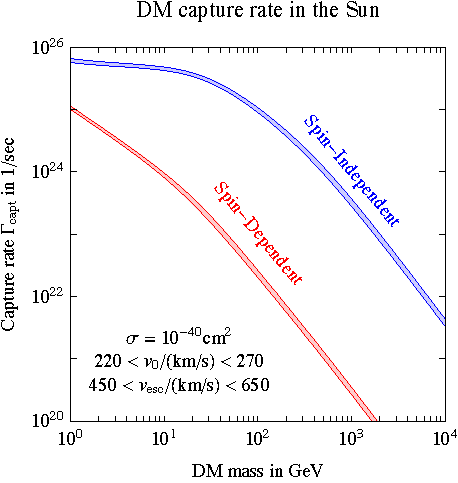
\includegraphics[width=0.48 \textwidth]{figs/GammacaptSISD}\qquad  
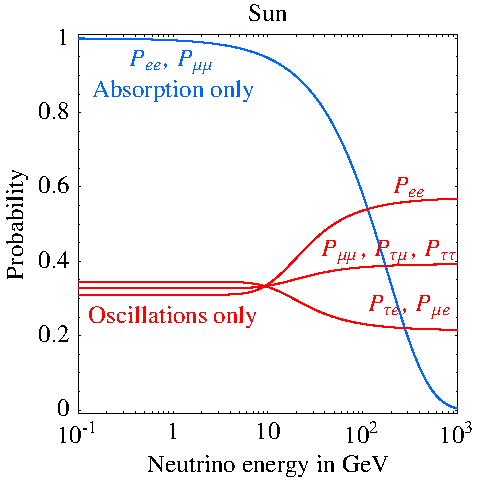
\includegraphics[width=0.50 \textwidth]{figs/OscAbsSun} $$
\begin{center}
\caption[Capture rate of DM particles in the Sun]{\em {\em Left:}
{\bfseries Capture rate}  of DM particles in the Sun, $\Gamma_{\rm capt}$.
The capture rate is linearly proportional to the DM cross-section on a proton, which we take to be $\sigma=10^{-40} \, {\rm cm}^2$  for both SI and SD scatterings. \label{fig:capturerate}
{\em Right}: 
Illustration of
{\bfseries the effects of oscillations and CC absorption} on the neutrino flux produced
 in the center of the Sun. Both the survival ($P_{\alpha\alpha}$) and transition ($P_{\alpha\beta}$) probabilities for different neutrino flavors are shown. 
 In the energy regime of interest for weak-scale DM,
  the oscillations and absorptions are equally relevant. High-energy neutrinos are absorbed significantly by solar matter.
 \label{fig:DMnupropagationinSun} }

\end{center}
\end{figure}



Fig.\fig{capturerate} (left) shows the total DM capture rate in the Sun for both spin-independent and spin-dependent scatterings of DM on nuclei. 
For concreteness, we set both the SI and SD cross section for scattering on a proton to $\sigma=10^{-40} \ {\rm cm}^2$.  
The total capture rate is the sum of contributions from scattering on different nuclei, each proportional to its respective $\sigma_i$. 
For SI interactions, several elements in the solar composition contribute in similar amounts, either because they are very abundant (He) or because they are heavy (Fe, O, Si, etc). In contrast, for the SD case, the capture rate is  dominated by hydrogen, with nitrogen playing a minor role.

\smallskip

For heavy DM, $M \gg m_i \sim 100\GeV$,
DM can be captured only if it is very slow, 
$ v< 2v_{\circledast\rm esc}\sqrt{m_i/M}$.
Consequently, in this limit the capture rate is proportional to $1/M^2$,
\beq 
\label{eq:GammaCaptApproxNumbers}
\Gamma_{\rm capt} \approx
\frac{ 5.9 ~ 10^{22}}{\rm sec} \left(\frac{\rho_{\rm DM}}{0.3 \, \sfrac{\rm GeV}{\rm cm^3}}  \right) 
\left(\frac{100\, {\rm GeV}}{M} \right)^2 
\left(\frac{270 \, \sfrac{\rm km}{\rm sec}}{ v_0} \right)^3 
\frac{\sigma_{\rm SD} + 1200\ \sigma_{\rm SI} }{10^{-40}\,{\rm cm}^2},
\eeq
having approximated DM interactions with nuclei as a spin-dependent and a spin-independent
cross section on nucleons (section~\ref{sec:DMscatt:nuclei}).


\medskip

As an aside, it is worth noticing that the SI capture rate is about 3 orders of magnitude larger than the SD one (assuming equal scattering cross sections, $\sigma_{\rm SI}=\sigma_{\rm SD}$). This is evident both in figure \ref{fig:capturerate} (left) and in the approximate formula in eq.~(\ref{eq:GammaCaptApproxNumbers}). 
Consequently, the expected neutrino signal 
for the SI case is larger by the same factor, and the bounds on SI scattering cross section about
3 orders of magnitude stronger. This is consistent with the results presented in fig.s~\ref{fig:sigmaSIbound} and \ref{fig:DDSDbounds}. These figures also show that, as discussed in section \ref{sec:DMnustatus}, the bounds from nuclear recoil direct detection searches are very stringent for SI scattering, so that the solar neutrino bounds are competitive only for the SD case.



\subsection{Computation of the neutrino energy spectra}\label{sec:DMnuprop}
The neutrino energy spectra from DM annihilations in the Sun,
${dN_\nu}/{dE_\nu}$ in eq.\eq{nuflux},
are computed similarly to those in vacuum with two important differences.

\medskip

First, one needs to take into account that DM annihilations occur within the dense matter of the Sun. Such an environment has a number of important consequences
for the generated neutrino spectra. 
The hadrons produced in the annihilations shower and loose energy before they decay. Charmed and $b$-flavored hadrons are slowed down (to a different extent, $b$-hadrons are slowed more) and their energy distribution is reduced to a rapidly decreasing exponential as they move through solar matter. The neutrinos produced by the subsequent decays are therefore significantly less energetic than those produced by the same processes in vacuum. 
Positively charged pions and kaons lose significant energy and decay essentially at rest, producing monochromatic (in case of 2-body decays) or broader but still sharp (in case of 3-body decays) neutrino peaks.
Neutrons and negatively charged pions are  absorbed. The former create deuterons, the latter annihilate in nuclear matter. Negative kaons are captured. In these cases, very few or no neutrinos are produced.
The leptons, which are produced in the annihilation showers, are also affected significantly. Negative muons are mostly captured. Positive muons are stopped and decay at rest. Taus, which have a shorter lifetime than muons, lose some energy before decaying.
In addition, the struck nuclear matter can also produce unstable particles that create fluxes of secondary neutrinos.
These complex processes can be modeled using dedicated MonteCarlo tools. 

In summary, particles with a large cross section and/or long lifetimes 
tend to dissipate energy or even stop before decaying into neutrinos.  
Their decays give rise to large neutrino fluxes at low energies, typically below the detection threshold of large neutrino telescopes such as {\sc Icecube}, but possibly within the sensitivity of {\sc SuperKamiokande} \cite{Bernal:2012qh}. The high energy portion of the spectra, although reduced and smoothed out relative to 
 annihilations in vacuum, however, remains to be prominent. Figure \ref{fig:DMnuspectra} (left) shows an example of the resulting neutrino fluxes.

\medskip
 
 \begin{figure}[t]
$$
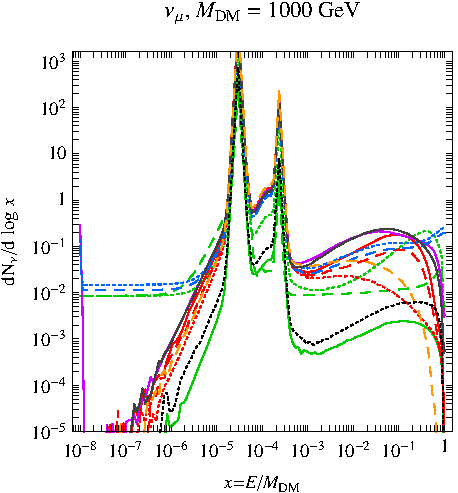
\includegraphics[width=0.32 \textwidth]{figs/prodnumu}\quad  
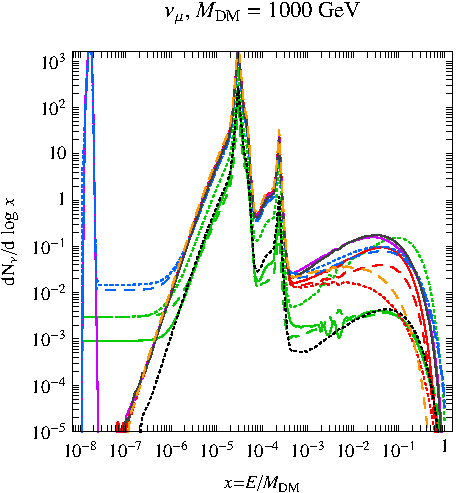
\includegraphics[width=0.32 \textwidth]{figs/detectnumu}\quad 
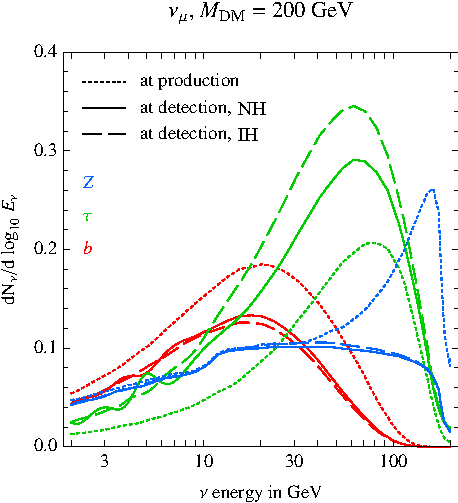
\includegraphics[width=0.31 \textwidth]{figs/finalnumu200mod}
$$
\begin{center}
\caption[Spectra of neutrinos from DM captured in the Sun]
{\em {\bfseries Spectra of neutrinos from DM captured in the Sun}. The color coding and style in the left and middle panels are the same as in figure \ref{fig:spectraatproduction}.
{\em Left}: $\nu_\mu$ spectra at production. The low energy peaks from the decays of stopped hadrons and leptons are clearly visible. 
{\em Middle}: $\nu_\mu$ spectra at detection, after propagation (interactions and oscillations, in solar matter, in vacuum and in terrestrial matter, assuming for definiteness normal hierarchy and neutrinos crossing vertically the Earth). 
{\em Right}: Direct comparisons of the $\nu_\mu$ spectra at production and detection, for a lighter DM particle and focusing on the energy range of interest for current neutrino telescopes. The considered annihilation channels are $ZZ$, $\tau^+\tau^-$ and $b\bar b$, and we show the results for both the normal  and inverted neutrino hierarchy. (Figures from \arxivref{1312.6408}{Baratella et al.~(2014)} in~\cite{DMnu}).
\label{fig:DMnuspectra}
}
\end{center}
\end{figure}


Second, one needs to take into account 
the series of phenomena that neutrinos undergo as they propagate from their point of origin at the Sun's core to their eventual detection on Earth.
These include: i) flavor oscillations within the Sun's matter, ii) interactions with the Sun's matter, iii) vacuum oscillations from the Sun to the Earth, and iv) oscillations within the Earth's matter, depending on the specific Earth segment traversed.
The interactions in the Sun include two types of processes.
First, there are neutral current interactions where neutrinos scatter inelastically off nuclei, leading to partial energy loss. 
 Second, there are charged current interactions, during which an incident neutrino scatters off a nucleus, subsequently producing a charged lepton and scattered hadrons.
 These leptons then decay back into neutrinos and anti-neutrinos of the same and different flavors, albeit of a lower energy. 
 In particular, when the initial neutrino is $\nu_\tau$ ($\bar\nu_\tau$), the produced $\tau^-$ ($\tau^+$) decays promptly before losing energy, giving rise to another $\nu_\tau$ and $\bar\nu_e, \bar\nu_\mu$ (respectively $\bar \nu_\tau$ and $\nu_e, \nu_\mu$): this is the {\em tau regeneration} phenomenon. 
Since the neutrino scattering cross sections increase with energy, high energy neutrinos are efficiently absorbed as a consequence of interactions with matter (see figure \ref{fig:DMnupropagationinSun} right) and their energy redistributed. Consequently, neutrinos produced in the center of the Sun only exit with sub-TeV energies.


Neutrino oscillations in the vacuum and within Earth's matter are governed by specific oscillation parameters commonly referred to as
$\Delta m^2_{\rm sun}$,
$\Delta m^2_{\rm atm}$, $\theta_{12}$, $\theta_{23}$, $\theta_{13}$~\cite{NuOsc}, 
including the still uncertain neutrino mass hierarchy (`normal' or `inverted'). Inside the Sun, both coherent flavor oscillations and coherence-breaking interactions affect  neutrino propagation and are equally important, as illustrated in figure \ref{fig:DMnupropagationinSun} (right). 
Hence, a suitable formalism that includes both of these effects is required for a correct description. 
A mostly analytical method consists of studying the spatial evolution of the $3 \times 3$ matrix of neutrino densities, $\rho(E_\nu)$, and anti-neutrino densities, $\bar\rho(E_\nu)$. The diagonal entries of the density matrix represent the population of neutrinos of the corresponding flavor, whereas the off-diagonal entries quantify the quantum superposition of neutrino flavors. 
Using this formalism one finds that the fast oscillations average the off-diagonal elements to zero, without encoutering numerical issues.
An alternative approach calculates probabilities using 
a  fully numerical  MonteCarlo simulation that follows the path of a single neutrino undergoing oscillations and interactions.
The two approaches yield results that are in agreement for all practical purposes.

In summary, 
propagation affects neutrino fluxes in three primary ways: it attenuates the fluxes, reshuffles neutrino flavors, and reduces neutrino energies. 
The  middle panel in figure \ref{fig:DMnuspectra} shows an example of the resulting neutrino spectra after propagation, 
while the right panel shows the relative importance of propagation, 
albeit, for a lower value of $M$.
The suppression of the high energy end of the neutrino spectrum is evident.
The noticeable fluctuations around a few GeV can be attributed to the effects of flavor oscillations.
Oscillations can also enhance the flux of a specific neutrino flavor,
as showcased by the $\tau$ annihilation channel in the right panel in figure \ref{fig:DMnuspectra}.



\section{DM in stars}\label{sec:DMinstars}
\index{Stars!indirect detection}\index{DM capture!stars}\index{Indirect detection!stars}
Several scenarios have been considered in which DM particles are captured inside stars (the Sun, white dwarfs or neutron stars)~\cite{DMinstarsReviews}. 
In this section we therefore generalize the discussion from the previous section, and summarize the main possibilities of capturing DM in stars and its phenomenology. See also \arxivref{2307.14435}{Bramante and Raj} in~\cite{otherpastDMreviews} for a dedicated review.





\subsection{Other signals from DM capture in the Sun}\label{sec:DMnuother}\index{Sun!DM capture}
Extending the discussion of section \ref{sec:DMnu} beyond minimal models, one can consider the possibility that
the DM particles captured in the Sun {\bf annihilate into new hypothetical long-lived particles}.
For example, {\em `secluded DM'} or {\em `dark sector'} models (see section \ref{sec:darksectors}) involve metastable mediators~\cite{secludedDMandDMnu}.
These mediators can escape from the dense solar core and subsequently decay into Standard Model particles. Depending on their lifetime, the decays can occur either in the outer layers of the Sun or in the empty space outside the Sun. 
In the former case, neutrinos remain the only particles that make it out of 
the Sun, however the signal is modified. In particular, the 
 interactions of neutrinos with solar matter are less important 
 so that neutrinos with higher energy can now escape, 
unlike in the scenarios involving DM annihilations in the solar core.
If the mediators decay outside the Sun,
these decays can result in gamma rays and charged particles, which can  then be searched for. {\sc Antares}, {\sc Hawc}, {\sc Fermi} and {\sc IceCube} have put bounds on the neutrinos and gamma rays originating from these scenarios~\cite{secludedDMandDMnu,secludedDMsolarbounds}.

\medskip

The accretion of 
DM particles can result in
an unconventional energy transport mechanism 
in the Sun's interior~\cite{DMinsun1}. 
Because of their large mean free path, DM particles can efficiently transport energy radially (provided that they do not annihilate away too quickly), transferring heat from the deeper layers of the Sun to the external ones. This would {\bf lower the temperature of the Sun's core}, leading to a decreased solar neutrino flux. 
Historically, in the 1980's, this mechanism was  proposed as a solution to the solar neutrino problem (the deficit of neutrinos with respect to the predictions of the standard solar model) in the so-called {\em cosmion} model (WIMP-like particles with a mass of a few GeV and a now-excluded large cross-section $\sim 10^{-36} \ {\rm cm}^2$ for scattering on nuclei). The idea was abandoned when neutrino flavor oscillations were shown to be the explanation of the deficit. 


The idea was revived around 2010 \cite{DMinsun2}, to possibly explain the
 `{\em solar composition problem}'  (or the `{\em solar abundance problem}').
  This problem pertains to the disagreement between the determinations of the Sun's heavy element content from helioseismological data and the standard solar model predictions.
 One potential explanation centered on light asymmetric DM (see section \ref{sec:AsymmetricDMth}), which by definition does not annihilate, and would therefore accumulate significantly in the solar core. The same line of reasoning was also used to derive constraints on WIMP-like DM.
Subsequent careful studies showed, however, that the effect is too small to have any observable impact, at least for choices of parameters that are compatible with direct detection constraints. 
Nevertheless, for certain scenarios involving speed- or momentum-dependent DM scattering, or long-range interactions, the effects may still be significant.


\subsection{DM capture in other stars}\label{sec:CaptureStars}

DM capture can become more significant for stars with characteristics that are more extreme than those of the Sun, or located in more extreme environments. 

\smallskip

For {\bf solar mass stars} \cite{DMinSunlikeStars}, 
DM capture effects begin to be significant when 
these are immersed in a DM halo with density $\rho_{\rm DM} \gtrsim 10^3 - 10^5 \, {\rm GeV}/{\rm cm}^3$ (depending on the effect), which is possibly realized
close to the Galactic Center. There are two 
primary scenarios:
\begin{enumerate}
 \item If DM particles annihilate, the consequences of DM capture depend on
 the amount of energy that DM annihilations inject into the stellar core, which in turn depends on the precise values of the environmental DM density, the DM speed distribution, the scattering cross section controlling the DM capture rate, and the mass and the composition of the star. 
Generally speaking, the energy released by DM annihilations extends the lifetimes of stars
by counteracting the gravitational contraction and by contributing to the hydrostatic equilibrium balance. In optimal circumstances, a star could remain frozen in its evolution longer than 
the age of the Universe, in a condition that has been termed the {\bf DM burner}. 
For red giant stars, the implications are similar but tend to be less pronounced.
If DM is dissipative, the accumulation of DM is more efficient and the effects larger (see \arxivref{2203.09522}{Peled and Volansky (2022)})~\cite{DMinSunlikeStars}.
However, given the complexity of stellar evolution, the detailed dependence on the parameters, and the difficulty of observing relatively normal stars very close to the GC, it is difficult to draw generic conclusions or bounds.


Early very massive stars, referred to as {\bf Population III stars} (see more extensive discussion in section \ref{sec:DarkStars} below), can also
become DM burners by capturing massive quantities of DM, 
given that they formed in a dense DM environment at a high redshift~\cite{DMinPopIIIStars}. If they burn DM, they can survive until the present epoch, and can be searched for as an anomalous stellar population: they would appear much larger and with a considerably lower surface temperature compared to normal stars with the same mass and metallicity. 
Due to the absence of reliable observations, and given the large dependence on the astrophysical parameters, no firm conclusions or bounds can be drawn on DM properties from this.  


\item 
If DM particles do not annihilate, as is the case, for instance, for asymmetric DM (see section \ref{sec:AsymmetricDMth}), they accumulate in the central region of the star.
The accumulated DM can facilitate the transfer of energy towards the outer layers, similar to the scenario described for the Sun in section \ref{sec:DMnuother}.
 While the effects on the Sun are mostly negligible, stars situated within dense DM environments can experience significant heat transport, leading to notable alterations in their evolutionary path.
The net effect is  somewhat opposite to the case of the DM burner;
the star has to increase its core nuclear burning intensity to compensate for the reduction in temperature caused by the DM transport, therefore modifying its position in the main sequence of the Hertzsprung-Russel diagram, making itself recognizable (bigger and more luminous),\footnote{In principle, this also alters the star's neutrino output, although such change we are unable to detect.}
as worked out in particular by \arxivref{1103.4384}{Iocco et al.~(2012)} \cite{DMinSunlikeStars}. 
However, no conclusive evidence of such peculiar stars has been presented to date.



\end{enumerate}


\subsection{DM capture in white dwarfs}\label{sec:CaptureWD}
\index{DM capture!white dwarfs}\index{Indirect detection!white dwarfs}\index{White dwarf}
White Dwarfs (WD) 
represent the final evolutionary stage for stars with mass $M_{\rm wd}$ below the Chandrasekhar limit\footnote{
Chandrasekhar originally derived this limit by modelling electrons as an ideal Fermi gas, and also derived its approximate dependence on fundamental constants, $M_{\rm Pl}$ and $m_p$.
} of
$1.44 \, M_\circledast \sim M_{\rm Pl}^3/m_p^2$, 
meaning that these majority of stars lack the mass to collapse into either a neutron star or black hole.
Instead, the gravitational collapse of the stellar core remnant is halted by the degeneracy pressure of non-relativistic electrons.
As a result, the stellar mass ends up concentrated in a radius $R_{\rm wd} \sim M_{\rm Pl}/m_e m_p$, comparable to the Earth's radius.\footnote{This radius
can be estimated by minimising $U_{\rm gravity} \sim -M/M_{\rm Pl}^2 R$ plus $U_{\rm quantum} \sim Q^{5/3}/m_eR^2$ where
$Q \sim (M_{\rm Pl}/m_p)^3$ is the Chandrasekhar bound on the number $Q$ of electrons and protons.}
White dwarfs are mostly composed of the last element which could be burnt by the progenitor star --- this element varies with the progenitor's mass, being helium for lighter stars and either carbon or oxygen for the more massive ones. 
Survey data indicate that the white dwarf mass distribution is peaked at $ 0.6 M_\odot$.
A white dwarf possesses a non-relativistic escape velocity, $v_{\rm esc} \sim \sqrt{2 m_e/m_p} \sim 0.03$.
The rough estimate $\rho_{\rm wd} \sim 3m_e^3 m_p/4\pi  \sim {\rm few} \ 10^{6}\,{\rm g/cm}^3$ for the white dwarf density shows that it is
parametrically higher than the density of ordinary matter, 
estimated as approximately
$\rho_{\rm ord}\sim \alpha^3 \, m_e^3 m_p\sim {\rm few} \,{\rm g/cm}^3$,  where $\alpha$ is the fine structure constant.

\smallskip



The computation of DM capture in white dwarfs proceeds similarly to that in the Sun or ordinary stars, 
with the advantage that the higher escape velocity in white dwarfs compared to stars enhances the DM capture rate, see eq.\eq{GammaCaptApprox} or \eqref{eq:Gamma:capt:Sun}.
One needs to take into account the peculiar core composition of white dwarfs, and DM capture due to scattering on the degenerate electron sea  can also be considered.
As discussed in section~\ref{sec:CaptureStars}, DM capture in such bodies can lead to two distinct observable consequences:
\begin{enumerate}

 \item {\bf If DM particles annihilate,} the impact of energy injection\footnote{The case in which annihilations occur into relatively long-lived mediators that decay outside of the star has been addressed by \arxivref{2309.10843}{Acevedo, Leane and Santos-Olmsted (2023)}~\cite{DMinWD}. In this case, which is equivalent to the one discussed in section \ref{sec:DMnuother} for the Sun, no energy is injected in the star. Instead, the decays of the mediators produce $\gamma$-rays that can be searched for.}
 is more significant in white dwarfs compared to stars, owing to the lower temperatures of white dwarfs.
 The WD can become a {\bf DM burner}~\cite{DMinWD}:
 it possesses an internal source of energy despite the depleted 
 nuclear fuel. Consequently, its surface temperature can rise to $1.4 \ 10^5\,{\rm K}$, which is at the upper end of the normal range: typical white dwarfs have surface temperatures in the range  
 $(0.8-4)\,10^4$ K. Observations of old, but still relatively hot WDs, could thus 
 provide a valuable test of these scenarios.
 In turn, the observations of WDs that are not anomalously luminous  can constraint DM properties. \arxivref{1906.04204}{Dasgupta et al.~(2019)} and \arxivref{2104.14367}{Bell et al.~(2021)}~\cite{DMinWD} used the observations of WDs in the globular cluster M4 to derive bounds on the spin-independent DM-nucleon cross section, as well as on the SI DM-electron scattering cross section. The respective bounds are of the order of $\sigma_{\rm SI}< 10^{-(42-44)} \ {\rm cm}^2$ (for $100 \ {\rm keV} \lesssim M \lesssim 100$ TeV) and $\sigma^{\rm el}_{\rm SI} < 10^{-41} \ {\rm cm}^2$ (for $M \gtrsim 100$ MeV). 
The bounds on $\sigma_{\rm SI}$ are less stringent than the ones from direct detection experiments, for electroweak scale DM masses, see fig.~\ref{fig:sigmaSIbound} (bottom).
However, the WD bounds extend to much lighter DM masses (for which, however, evaporation needs to be carefully taken into account), and are also more stringent for heavier DM. 
In contrast, the WD constraints on DM-electron scattering are more stringent than direct detection bounds
over the whole applicable DM mass range, see fig.~\ref{fig:DDSIelec:bounds}. 
Nevertheless, the WD limits warrant caution due to ongoing discussions on the DM composition in globular clusters, as briefly touched upon in section~\ref{sec:IDgamma}. Since WDs are assumed to be composed solely of one of the following elements, ${}^4$He, ${}^{12}$C or ${}^{16}$O, all of which have spin-less nuclei, no bounds on SD scattering can be placed using these observations.



 \item {\bf If DM annihilations are negligible}, 
DM accumulates in the core of the white dwarf. Even a small amount of DM
(so that the total mass of WD-captured DM, $M_{\rm DM}$, satisfies   $M_{\rm DM}\ll M_{\rm wd}$)
can trigger a {\bf Type-Ia supernova explosion} of WD~\cite{aDMinWD}. 
Since evaporation is not relevant for large DM masses (see the discussion in page~\pageref{vescSun} for the case of the Sun), the captured DM particles rapidly fall to the centre of WD, forming a thermal sphere with radius (see eq.~(\ref{eq:n(r)}))
\beq r_{\rm DM} \sim \left(\frac{3 \, T_{\rm wd}}{2 \pi \, G \rho_{\rm wd}M}\right)^{1/2} \sim 300\, {\rm m}\qquad
\hbox{for $T_{\rm wd} \sim 10^7\,{\rm K}$ and $M\sim 10^6\GeV$,}\label{eq:RDMwd}\eeq
where $T_{\rm wd}$ is a typical core temperature and $\rho_{\rm wd} \sim 10^6$ g/cm$^3$ a typical core density.
Notice that `normal' stars have a much 
lower core density and also a somewhat higher core temperature. This implies that in white dwarfs DM capture (eq.~(\ref{eq:C_A})) is more efficient and the DM sphere more compact.
This is why white dwarfs, and compact objects in general, can give stronger constraints on DM than ordinary stars.


If the DM density $M_{\rm DM}/r_{\rm DM}^3$ exceeds the matter density of the host white dwarf, 
then DM starts self-gravitating and collapses, possibly forming a small black hole.
The thermal energy released during the collapse can trigger nuclear fusion and therefore ignite a supernova explosion. Alternatively, the black hole forms, and its subsequent evaporation triggers the supernova explosion.\footnote{If DM is bosonic and $ T < T_{\rm BEC} \sim n^{2/3}/M$, then DM does not have 
a thermal Maxwellian distribution, but rather
forms a Bose-Einstein condensate (BEC). The DM sphere 
has a smaller radius
$R_{\rm BEC} \sim (G M^2 \rho_{\rm dw})^{-1/4}$,
and forms a black hole more easily.
If the black hole is big enough to undergo the Bondi-Hoyle accretion
until it engulfs the white dwarf, instead of evaporating through Hawking radiation, 
$\dot M_{\rm BH} \sim -M_{\rm Pl}^4/M_{\rm BH}^2$, this also leads to bounds on the DM parameter space, which are, however, rather complex (see, e.g.,~\arxivref{1905.00395}{Janish et al.~(2019)} in~\cite{aDMinWD}).} 
Observations of specific white dwarfs, which remained stable and did not explode, combined with the recorded supernova rates, provide evidence against this scenario. The
 resulting bounds on the SI or SD DM-nucleon scattering cross section $\sigma_{\rm SI,SD}^{N}$
can be stronger than the bounds from direct detection~\cite{aDMinWD}. 
They are relevant for $M \gtrsim 10^6$ GeV and can reach $\sigma_{\rm SI,SD}^{N} \sim 10^{-43}$ cm$^2$,
as plotted in fig.\fig{sigmaSIbound}.
\end{enumerate}



\subsection{DM capture in neutron stars}\label{sec:CaptureNS}\index{Neutron star}\index{DM capture!neutron stars}\index{Indirect detection!neutron stars}
DM capture can be even more important for  denser compact objects such as
neutron stars (NS). These are remnants of massive super-Chandrasekhar
stars, originally possessing a mass typically between 10 and 25 $M_\circledast$, which underwent a supernova explosion. 
Neutron stars are supported by neutron degeneracy pressure.
Estimates analogous to white dwarfs in section~\ref{sec:CaptureWD} apply, with $m_e$ replaced by $m_n$.
That is, neutron stars have a typical radius of $R_{\rm ns} \sim M_{\rm Pl}/m_n^2\sim 10 \,{\rm km}$, 
a mass around $M_{\rm ns} \sim 1.4  M_\circledast$
and density $\rho_{\rm ns} \sim m_n^4 \sim 10^{15}\,{\rm g/cm}^3$ close to that of nuclear matter.
This predicted large $\rho_{\rm ns}$ density is observationally confirmed by the existence of
pulsars with fast $T \sim{\rm ms}$ period,
as the centrifugal force would exceed the gravitational force if $T \lesssim M_{\rm Pl}/\sqrt{\rho_{\rm ns}}$:
fast-spinning gravitational stable bound states must be dense.
The total number of nucleons is $N_{\rm ns} \sim (M_{\rm Pl}/m_n)^3 \sim 2 \, 10^{50} $.
Since there are no small parameters,
the escape velocity $v_{\rm esc}^2 \approx 2 G \, M_{\rm ns} /R_{\rm ns} $ is comparable to the speed of light. 
Gravity is so strong that DM particles attracted within the impact parameter ($v$ is the DM speed in the halo, far from the star)
\beq\label{eq:bns}
\frac{b}{R_{\rm ns}}= \frac{v_{\rm esc}/v} {\sqrt{1-v_{\rm esc}^2 }},
\eeq
 hit the neutron star with relativistic energy,  $E\sim \gamma M$, where $\gamma \sim 1.3 $.
DM is accreted at a rate
$ \sfrac{dM_{\rm DM}}{dt} \sim \rho_{\rm DM} v \, \pi b^2\, \min\left(1, \sfrac{\sigma_N}{\sigma_*}\right)$.
Over a time interval $\Delta t$ this results in a total accumulated DM mass of
\beq
M_{\rm DM} 
\sim 10^{11}\,{\rm kg}  \frac{\rho_{\rm DM}}{0.3\GeV/\cm^3} \frac{\Delta t}{10^{10}\,{\rm yr}}
\frac{b^2}{R^2_{\rm ns}}
 \min\left(1, \frac{\sigma_{\rm SI,SD}^n}{\sigma_*}\right).
 \eeq
Here, $\sigma^n_{\rm SI,SD}$ is the SI or SD DM/neutron cross section and 
$\sigma_*$ its critical value above which
all DM that hits the neutron star gets geometrically captured
\beq
\sigma_* \sim \frac{\pi R^2_{\rm ns}}{N_{\rm ns}}\sim 10^{-44}\,{\rm cm}^2.
\eeq
That is, DM is captured even for very small values of $\sigma_* $, 
comparable to bounds from direct detection searches.


The captured DM can lead to several potentially observable signatures, listed below. 
While the first two are extensions of those discussed for other astrophysical bodies in preceding subsections, the third is specific to neutron stars.
\begin{enumerate}
\item \label{DMinSN1} \index{Neutron stars!DM annihilations}
{\bf If accumulated DM particles {\em annihilate}}, the neutron star achieves the condition of {\bf DM burner}, 
and its surface temperature increases~\cite{DMcaptureinNSandannihil}. 
Neutron stars form at large temperature $T \sim m_n$ and then undergo cooling, initially due to neutrino emissions and later because of photon emissions. 
In the absence of heating processes, temperatures below 1000 K are reached after about $10\,{\rm Myr}$. 
Detecting old neutron stars with surface temperatures somewhat higher than this would allow to probe this scenario. 



\item {\bf If accumulated DM particles {\em do not annihilate}} \cite{DMcaptureinNSandcollapse}, 
they form a thermal sphere at the center, with a radius $r_{\rm DM} \sim 30$ cm for $T_{\rm ns} \sim 10^5$ K and $M \sim 100$ GeV. 
{\bf A  black hole eventually forms} and consumes the neutron star. 
The mere existence of neutron stars in various DM backgrounds (i.e., the fact that they were not destroyed by DM),  allows to place stringent constraints on the DM/neutron scattering cross section. The detailed bounds (see in~\cite{DMcaptureinNSandcollapse}) depend on many parameters, including whether or not a Bose-Einstein condensate of DM forms, similar to the situation in white dwarfs. 
The bounds derived by \arxivref{1706.00001}{Bramante et al.~(2018)}~\cite{DMcaptureinNSandcollapse} reach $\sigma_{\rm SI,SD}^{N} \sim 10^{-47}$ cm$^2$ for $M \approx 10^{10}\GeV$,
as plotted in fig.\fig{sigmaSIbound}. 
\arxivref{1812.08773}{Garani et al.~(2018)} find even stronger constraints in some specific configurations.

\item 
\label{DMinSN2}\index{Neutron stars!DM kinetic heating}
Regardless of whether they eventually annihilate or not, captured DM particles get accelerated to relativistic speeds, fall onto the neutron star and deposit their kinetic energy. 
This {\bf DM {\em kinetic} heating of neutron stars}~\cite{DMkineticheatingNS} keeps the surface at a temperature 
$T_{\rm surface} \approx (\rho_{\rm DM}/ v_{\rm DM})^{1/4} $
(about $1700\,{\rm K}$ for neutron stars in our vicinity),
for which the heating rate $dE_{\rm DM}/{dt}$ is in equilibrium with the
photon emission rate,
$W= 4\pi R^2 \, \pi^2 T_{\rm surface}^4/60$.
This happens if $\sigma_{\rm SI,SD}^n\circa{>} \sigma_*$ and $\GeV \circa{<}M \circa{<}\,{\rm PeV}$.
The mass range can be understood as follows.
Upon single scattering, a falling DM transfers to neutrons an energy
\beq \Delta E  = \frac{m_n \gamma^2 v_{\rm esc}^2}{1+ m_n^2/M^2 + 2\gamma m_n/M} \langle 1- \cos\theta_{\rm CM}\rangle,
\eeq
which is larger than the redshifted kinetic energy of the free DM,
$\gamma M v_{\rm esc}^2/2$, if $M \circa{<} 10^6\GeV$.
For larger $M$ multiple scatterings are needed to capture DM, and as a result 
$\sigma_*$ 
increases as $M/10^6\GeV$ for heavier DM.
On the other hand, for $M \circa{<}m_n$ the transferred energy $\Delta E$ is so low that due to Pauli blocking
(in a neutron star the neutrons occupy energy levels up to the Fermi momentum of about $m_n$)
$\sigma_*$ increases as $m_n/M$, if DM mass is lowered.

\item {\bf MeV to GeV DM} that interacts strongly could detectably alter the structure of neutron stars~\cite{1803.03266}.
\end{enumerate}

\smallskip

Next, we discuss the observational status of items~\ref{DMinSN1} and~\ref{DMinSN2}.
Presently, meaningful tests are still lacking, since the observational sensitivities to the temperature of neutron stars 
tend to be about a factor of 20-100 higher than the expected effects due to DM.
The James Webb Space Telescope could observe $T \sim 2000$ K for certain nearby neutron stars.


Furthermore, there exist various sources of backgrounds. 
Neutron stars could be heated by other mechanisms, such as the conversion of
their rotational energy trough magnetic fields, 
or due to the accretion of normal matter onto their surface
(resulting in pronounced heating of the magnetic poles), crust cracking, vortex friction, etc.
It is therefore essential to focus on isolated neutron stars situated in regions where DM density surpasses that of normal matter.
In the interstellar medium, DM and matter densities are comparable, which could potentially obscure any additional heating effects due to DM. 
Fortunately, $X$-ray data suggest that 
since about 10 Myr the Sun has resided in a `local bubble'
where the matter density is nearly a factor of 100 less than the average. 
In this environment, DM annihilations would heat neutron stars up to $\sim 2500$ K.

Should future telescopes be able to test neutron star heating due to DM, 
the DM/nucleon cross sections will be probed down to
$\sigma_{\rm SI, SD}^N \lesssim 10^{-46}$ cm$^2$ for $1 \ {\rm GeV} \lesssim M \lesssim 10^6$ GeV~\cite{DMcaptureinNSandannihil,DMkineticheatingNS}.
This surpasses current spin-dependent direct detection bounds, while it is not competitive with the spin-independent bounds.
Nevertheless, such findings would still be interesting, since, as discussed in section~\ref{chapter:direct},
various effective operators induce small direct detection cross sections, suppressed 
by the DM velocity or momentum transferred.
These suppressions are lifted in relativistic collisions of DM on neutron stars.
For non-minimal models, such as inelastic DM (section~\ref{sec:inelasticDM}),
relativistic DM collisions on neutron stars would probe much higher DM inelasticities up to $\sim m_n$
(covering, for example, the mass splittings predicted by theories where DM is part of a single electroweak multiplet, see section~\ref{MDM}).



\subsection{Dark stars?}\label{sec:DarkStars}\index{Dark!star}\index{Stars!dark}
The role of DM in the formation and evolution of early stars has also been considered in depth. 
The first stars in the Universe, termed Population III stars, formed out of diffuse gas clouds situated within and concentric to large DM halos (typical mass of $\sim 10^6 \, M_\odot$, 
and composed of approximately $\sim85\%$ DM, consistent with the Universe's general composition). 
In the standard picture, 
both the DM halo and the gas cloud contract, and eventually the baryonic matter ignites nuclear fusion at the center of the cloud, which then hydrostatically supports the newly formed star, halting the collapse. 

Beginning in 2007, a series of works speculated that, instead, the DM halo concentration could ignite DM annihilations at its center. This would lead to a halt in the collapse of the gas cloud prior to the onset of nuclear fusion,
and to the formation of a pseudo-stellar object,  a `{\em dark star}' \cite{DarkStars}, composed of hydrogen and helium, 
and sustained by DM annihilations instead of nuclear fusion.
For this mechanism to work, a sufficiently high DM density is essential. Notably, in the early Universe, DM density was higher at redshift $z$ by a factor $(1 + z)^3$. Moreover, the first stars form exactly in the centers of their host DM halos, where the density is highest.
The process is sustained if the heat produced by DM is efficiently trapped inside the star (which is the case because of the high baryonic density,
akin to the Sun's core) so that the heating rate can be higher than the baryonic cooling mechanisms (which is found to occur when the gas density exceeds $10^{13}$ particles/cm$^{3}$ for a typical WIMP-like DM). Note also the conceptual difference with the `DM burner' case discussed earlier: in that case, DM particles accumulate in the center of early stars by scattering on the stellar matter, leading to DM capture, while in dark stars DM gets trapped during a concentric collapse. For DM capture, DM particles need to possess a significant scattering cross section with baryons, while dark stars can in principle be born even for mostly gravitationally-interacting DM, provided that it then annihilates into SM particles.
The canonical thermal relic cross section $\sim 2\, 10^{-26}\, {\rm cm}^3/{\rm s}$ in  eq.~(\ref{eq:sigmavcosmo}) is sufficient for the mechanism to work.


This unconventional stellar phase would start very early, at redshift $z \sim 10-50$, and could last for millions to billions of years, 
contingent on the availability of DM fuel. If would create anomalous stars with very heavy masses approaching $\sim1000 \, M_\circledast$, 
large sizes of up to $\sim 200 R_\circledast$, 
high luminosities up to $10^6 \, L_\circledast$ and a low surface temperature below $10^4$ K. 
These characteristics would make them observationally very distinct from standard Population III stars, and potentially detectable at very high redshifts with the James Webb Space Telescope. 
Dark stars can also alter the reionization history of the Universe
(negatively,
their low surface temperature implies that they would emit less ionizing radiation compared to normal Population III stars) and modify the cosmic microwave background~\cite{DarkStars}. 

Upon depletion of DM fuel, dark stars would 
transition into heavy main-sequence stars. The most massive among them would eventually collapse into anomalously massive black holes,
possibly providing a seed to the formation of early supermassive black holes.


\smallskip

Certain simulations \cite{DarkStars} claimed that dark stars do not form, although this could be due to their limited resolution.
Observationally, no evidence of dark stars has been found so far, and no general bounds have been derived, though
\arxivref{2304.01173}{C. Ilie et al.~(2023)}~\cite{DarkStars} proposed candidate objects consistent with dark stars.


\subsection{DM capture in planets}\label{sec:DMcaptureplanets}
Some of the physical concepts discussed above can be applied also  to the capture of DM by planets (the Earth, other solar system planets, or exoplanets), leading to noteworthy constraints~\cite{DMandplanets}.

\medskip

\begin{enumerate}
\item {\bf If DM particles can self-annihilate}, 
the energy deposition rate from the annihilation products should not exceed the measured {\bf {\em heat flow}} \, emanating from the Earth's interior. 
This was first noted by \arxivref{0705.4298}{Mack et al.~(2007)} and then refined and extended in \arxivref{1909.11683}{Bramante et al.~(2020)}. The constraints apply to DM masses $100 \ {\rm MeV} \lesssim M \lesssim 10^{10}$ GeV and span the very broad range $10^{-38} \ {\rm cm}^2 \lesssim \sigma_{\rm SI} \lesssim 10^{-16} \ {\rm cm}^2$ (for spin-independent scattering, see figure \ref{fig:sigmaSIbound}) and $10^{-33} \ {\rm cm}^2 \lesssim \sigma_{\rm SD} \lesssim 10^{-11} \ {\rm cm}^2$ (for spin-dependent scattering). 

Some pioneering studies~\cite{DMandplanets} also considered the heat flow from inside Jupiter, Saturn, Uranus and Pluto, 
but this did not yield particularly relevant constraints.
Similarly, the requirement that the DM heat injections did not halt the contraction of the proto-planetary gas cloud and thus the formation of Jupiter (or Jovian planets) allows to impose bounds, which are however not particularly competitive.

Recent investigations have also examined Mars and exoplanets. 
In the context of exoplanets, assuming that accurate temperature measurement will be possible (e.g.,~in the infrared with the James Webb Space Telescope), the sensitivity on the spin-dependent cross section on protons could reach $\sigma_{\rm SD}^p \lesssim {\rm few} \, 10^{-37} \ {\rm cm}^2$ for GeV and sub-GeV DM. 
This improved sensitivity compared to Earth observations can be attributed to the expected lower temperature of exoplanets, and to their large number. 


\item {\bf If DM particles do not annihilate,} they accumulate at the center of the planet and form a black hole, which again leads to constraints. For example, \arxivref{2012.09176}{Acevedo et al.~(2021)}~\cite{DMandplanets} determined  that DM with mass $10^7 \ {\rm GeV} \lesssim M \lesssim 10^{10} \ {\rm GeV}$ and spin-independent cross-section $10^{-32} \ {\rm cm}^2 \lesssim \sigma_{\rm SI} \lesssim 10^{-17} \ {\rm cm}^2$ is ruled out, otherwise the BH would have destroyed the Earth within a billion years. 
The updated analysis in \arxivref{2301.03625}{Ray (2023)}~\cite{DMandplanets} finds that celestial objects with large sizes and relatively low core temperatures, such as Jupiter, are more suitable and can exclude a slightly larger area of the parameter space. For even larger masses, and proportionally larger cross-sections, the BH would evaporate and overheat the planet. 

\end{enumerate}

\section{DM in the dark ages: CMB, reionization and heating}\index{CMB}\index{Indirect detection!CMB}
\label{sec:cosmoconstraints}
Dark ages are the epoch between recombination at $z \approx 1100$ and the formation of the first stars at $z \gtrsim 10$.  Annihilations or decays of DM particles during the cosmic dark ages inject energy into the medium, which causes
 heating and
additional ionization of the ambient hydrogen gas.
The resulting free electrons scatter on the CMB photons and modify the measured properties of the CMB, providing a mechanism 
 to probe the DM annihilation cross section or decay rate. 
The ensuing constraints are quite competitive with many of the other indirect detection bounds coming from the Galaxy or the local universe (see figures~\ref{fig:IDconstraints},~\ref{fig:IDconstraintsdecay} and~\ref{fig:IDconstraintssubGeV}), especially for light DM. 
They are also quite robust, i.e.,\ subject to a lesser extent to astrophysical uncertainties such as the DM distribution, the galactic propagation of cosmic rays and the environmental properties (galactic magnetic fields, ambient light distribution...). 
They do, however, remain sensitive to the velocity dependence of the annihilation cross-section, as we discuss below. 


\medskip

The fraction $x_{\rm ion}(z)$ of singly ionized atoms, which would normally hover around $10^{-4}$ for $z \lesssim$ few $10^2$ in the absence of exotic ionization processes, is 
affected by DM annihilations or decays. It follows the basic evolution equation 
\beq
\label{eq:xion}
n_{\rm A} (1+z)^3 \frac{dx_{\rm ion}(z)}{dt} = I(z)-R(z).
\eeq
On the right-hand side, we have the rate of ionization per volume $I(z)$, which tends to increase $x_{\rm ion}$, 
and the recombination rate per volume, $R(z) = R_{\rm H}(z) + R_{\rm He}(z)$, with which the hydrogen and helium atoms in the IGM recombine while ionization is ongoing. 
We omit the explicit expressions for these recombination rates here for brevity, but they can be found in the literature~\cite{reionbounds}.
The rate of ionizations per volume due to DM, at a given redshift $z$, is given by
\beq
\label{eq:Iion}
I(z) = \frac{\eta_{\rm ion}}{e_{\rm ion}} \frac{dE}{dt}(z),
\eeq
where $e_{\rm ion}$ is the average ionization energy per baryon (e.g.,\ 13.6 eV for hydrogen). 
The factor $\eta_{\rm ion}$ is the fraction of the energy that goes into ionizations, 
 while the remainder contributes to heating and atomic excitations. 
 The value of this fraction depends
 on $x_{\rm ion}(z)$ itself, and can in first approximation be taken to be (see, e.g., \arxivref{astro-ph/0310473}{Chen and Kamionkowski (2004)}~\cite{reionbounds} and references therein) 
\beq
\eta_{\rm ion} = \frac{1-x_{\rm ion}(z)}{3}.
\label{eq:etaion}
\eeq
The last term in eq.~(\ref{eq:Iion}) represents the energy injection rate from dark matter per unit volume. It is given by 
\beq
\label{eq:DMinjectionCMB}
\frac{dE}{dt}(z) = 
\left\{
\begin{array}{ll}
 \displaystyle \rho^2 (1+z)^6 f(z) \, \frac{\langle \sigma v \rangle}{M}  & {\rm (DM~annihilation)}, \\[3mm]
 \displaystyle \rho (1+z)^3 f(z) \, \Gamma & {\rm (DM~decay)}.
\end{array}
\right.
\eeq
Its form can be easily understood. 
Focusing on annihilating DM, the energy injection rate is determined by the number density of annihilating DM particles, $n=\rho/M$, squared, and rescaled to redshift $z$ by the factor $(1+z)^3$, multiplied by the probability of annihilations (given by the cross section $\langle \sigma v \rangle$), and by the energy injected in each annihilation (equal to $M$). 
One power of $M$ cancels in the final expression,  giving a rate proportional to $\langle \sigma v \rangle/M$. For decaying DM, the energy injection rate is proportional to  the decay rate $\Gamma$, and a single power of $n$, so that the dependence on $M$ completely cancels out. 
The factor $f(z)$ expresses the fraction of the total DM energy which is absorbed by the gas. It incorporates all the complexity of {\it how} the DM annihilation/decay products interact with the gas and {\it when} they do so. Distinct values of $f(z)$ can be calculated for various annihilation/decay species (e.g.,\ $e^\pm$, hadrons,\ldots, excluding neutrinos, which do not interact electromagnetically and therefore do not deposit any energy), 
for different spectra (the $dN/dE$ in eq.~(\ref{eq:primaryflux})), for different injection redshifts $z$, and taking into account that the absorption in general occurs at a later redshift $z^\prime$, after some cooling, etc.  Their values can be found tabulated in the literature 
(in particular \arxivref{1506.03812}{Slatyer (2016)} in~\cite{CMBbounds}).

In practice, it turns out that the impact of annihilating DM is well characterized by a single parameter: 
the excess ionization at redshift $z \sim 600$. For DM decay, the signal is similarly dominated by redshift $z \sim 300$. It is thus useful to introduce an effective redshift-independent factor  $f_{\rm eff}$. Note that this still depends on the specific DM particle physics model in a non-trivial way. 
The impact of DM annihilations can thereby be encoded in the factor $p_{\rm ann} = f_{\rm eff} \, \langle \sigma v \rangle/M$,
and in $p_{\rm dec} = f_{\rm eff} \, \Gamma$ for DM decays.




Based on these physical principles, the evolution equation (\ref{eq:xion}) can be solved for $x_{\rm ion}$ at any redshift $z>6$.\footnote{Below redshift 6 all the hydrogen and helium gas is assumed to be ionized, while helium is also doubly ionized below redshift $z = 3$, as suggested by the Gunn-Peterson test: the absence of absorption at Lyman-$\alpha$ frequency in the spectra of quasars located at $z<6$. Hence $x_{\rm ion}(z<6) \approx 1$.} This can be done at varying levels of refinement, either semi-analytically or using dedicated reionization codes such as {\tt Recfast}, {\tt HyRec} or {\tt CosmoRec}.   


\subsection{Optical depth}\label{sec:cosmoconstraintsCMBTau}
An initial series of studies determined DM constraints using a rather simplistic criterion that DM-induced free electrons should not alter the \textbf{optical depth}, experienced by CMB photons during their journey from the last scattering surface to us, beyond the measurements reported by CMB surveys like {\sc Wmap} or the more recent {\sc Planck} satellites~\cite{reionbounds}.
The optical depth
$\tau_{\rm op}$ is given by the integral (over the travel time of the photon) of the number density of free electrons $n_e(z)$, i.e., the scattering targets, multiplied by the Thomson scattering cross section $\sigma_{\rm T} = 8 \pi r_e^2/3 = 0.6652$ barn (with $r_e$ the electron classical radius) 
\beq
\tau_{\rm op} = - \int n_e(z)\, \sigma_{\rm T}\, \frac{dt}{dz},
\eeq
where $dt/dz$ is the standard $\Lambda$CDM relation between time and redshift in eq.~(\ref{eq:FRWexplicit}). In addition, $n_e(z) = n_{\rm A} (1+z)^3 \, x_{\rm ion}(z)$, where $n_{\rm A}$ is the number density of atoms today. The bounds obtained in this way constrain, for instance, $\langle \sigma v \rangle \lesssim 10^{-24}$ cm$^3$/s for $M \approx 100\GeV$.


\subsection{CMB anisotropies}
\label{sec:CMBconstraints}
\label{sec:cosmoconstraintsCMB}
\index{CMB!anisotropies}
A subsequent set of studies significantly improved the analysis by examining the effects of DM annihilations and decays on the  {\bf CMB anisotropies}~\cite{CMBbounds}. 
Rather than relying on the optical depth as a proxy, these works used detailed CMB codes such as {\tt Camb} or {\tt Class} to compute the modified power spectrum in presence of an increased ionization fraction, and compared with the refined {\sc Planck} data. 
The resulting bounds are discussed in section~\ref{sec:IDconstraints} and have gained significant traction in the literature. 
Note that the bounds on $\langle \sigma v \rangle$ scale linearly with $M$, while those on the DM decay 
lifetime 
$\tau$. 
These bounds are more stringent than those based solely on optical depth. For instance, they constrain $\langle \sigma v \rangle \lesssim 10^{-25}$ cm$^3$/s for $M \approx 100$ GeV.

\medskip

As mentioned above, the CMB bounds are robust with respect to many astrophysical uncertainties. Specifically, since the signal is dominated by high redshifts, 
prior to the onset of structure formation, the bounds do not depend on the details of DM distribution; the density $\rho$ in eq.~(\ref{eq:DMinjectionCMB}) is from the
smooth DM background, which is a well known quantity in the standard cosmology. That is, there is no need to specify the halo formation history, the halo profiles, etc.
However, for annihilating DM the CMB bounds do exhibit sensitivity to the velocity dependence of the annihilation cross section. 
For $p$-wave  DM annihilation, i.e.,~$\langle \sigma v \rangle \propto v^2$, these bounds weaken considerably, because the energy injection from DM gets suppressed due to DM being very cold (slow) during the dark ages. Put differently,  a large present day annihilation cross section is still allowed, because it was suppressed during the dark ages. 


\subsection{Temperature of the intergalactic medium}\index{Indirect detection!intergalactic medium}
\label{sec:boundsTigm}

A (smaller) series of studies explored the effect of DM energy injection on the {\bf temperature of the intergalactic medium} $T_{\rm igm}$~\cite{TIGMbounds}. 
Existing measurements of $T_{\rm igm}$ place direct constraints on the maximal allowed DM-induced heating. Moreover, if the temperature of the IGM is too high, gas clouds would not collapse and star formation would be delayed or impeded, allowing to impose indirect constraints on DM. 




The temperature $T_{\rm igm}$ follows a basic evolution equation somewhat analogous to eq.~(\ref{eq:xion}),
\beq
\label{eq:Tigm}
n_{\rm A} (1+z)^3 \frac{dT_{\rm igm}(z)}{dt} = - X(z) + C(z) + W(z)  .
\eeq
The first term on the r.h.s. describes the usual (adiabatic) cooling of the gas due to the expansion of the Universe. It reads $X(z) = 2 n_{\rm A} H(z) (1+z)^{3/2} \, T_{\rm igm}(z)$ and would lead to $T_{\rm igm}(z) \propto (1+z)^2$. 
The second term, $C(z) \propto T_{\rm CMB}(z) - T_{\rm igm}(z)$, accounts for the coupling between the inter-galactic gas and the CMB photons, that have a redshift-dependent temperature $T_{\rm CMB}$. When the inter-galactic gas is hotter than the surrounding CMB, some of its energy is transferred to the photons and therefore the gas `Compton-cools'. Conversely, if the gas is colder than the CMB, it heats up. 
The $C(z)$ term is only sketched here: we refer to the relevant literature for its precise form and the details concerning its derivation.\footnote{The same physics is relevant for the 21 cm measurements, in which an anomaly has been detected by {\sc Edges}, see section \ref{sec:EDGESanomaly}.}
The third term on the  right side of eq.~\eqref{eq:Tigm} encodes the warming of the inter-galactic gas due to DM energy release, and can be expressed as 
\beq
W(z) =  \frac{2}{3} \eta_{\rm heat}(z) \frac{dE}{dt}(z),
\eeq
where, similarly to eq.~(\ref{eq:etaion}), the factor
\beq
\eta_{\rm heat} \big(x_{\rm ion}(z)\big) = K \left[ 1- (1-x_{\rm ion}^a)^b \right],
\eeq
expresses the fact that only a fraction of the DM injected energy goes toward heating. Here, $K = 0.9971$, $a=0.2663$, and $b=1.3163$ are the values estimated in the literature.


Solving the coupled\footnote{The equations are coupled since $T_{\rm igm}$ enters the expressions for the recombination rates $R(z)$. The recombination codes mentioned above also allow to calculate the modified temperature history. The {\tt DarkHistory} code does an even more refined job.} differential equations (\ref{eq:xion}) and (\ref{eq:Tigm}), with appropriate expressions for the $f(z)$ factors relevant for heating, allows to obtain a prediction for $T_{\rm igm}(z)$ in the presence of DM as an exotic source of heating. 
Unlike in the CMB case, however, the potentially observable modifications to the temperature history depend primarily on physics at much lower redshifts, and therefore are very sensitive to structure formation history. The density $\rho$ in eq.~(\ref{eq:DMinjectionCMB}) has to be multiplied by a boost factor $B(z)$ which takes into account the DM collapse into gravitationally bound structures, their abundance, their density profile, etc. 
The resulting bounds on the DM annihilation or decay rates are weaker than those derived from the  optical depth constraint, and therefore also less competitive than those from the CMB. For instance, they constrain $\langle \sigma v \rangle \lesssim 2 \, 10^{-23}$ cm$^3$/s for $M \approx 100$ GeV, for DM annihilations into $\mu^+\mu^-$ and assuming an NFW profile for the DM halos.




\section{DM and Big Bang Nucleosynthesis}\index{Indirect detection!BBN}\index{Big Bang Nucleosynthesis}
\label{sec:BBNconstraints}
Historically, BBN 
has been pivotal in providing evidence for Dark Matter (DM), as discussed in section~\ref{sec:BBN}. 
Subsequently, BBN has also been employed to probe DM properties and establish constraints, which we briefly overview in this section~\cite{BBNbounds}.

\medskip


To begin with, let us consider the case of {\bf weak-scale Dark Matter}. The injection of particles from DM annihilations or decays during or immediately after BBN  
can lead to the destruction of some species of the newly formed light nuclei and to the overproduction of others, thereby altering their final abundances, and potentially spoiling the agreement with observations.
 This process is conceptually similar to DM energy injection during the dark ages,
 discussed in section \ref{sec:cosmoconstraints}. The differential equations to be solved here, the analogues of eq.s~(\ref{eq:xion}) and (\ref{eq:Tigm}) in section~\ref{sec:cosmoconstraints}, 
are those governing the relative abundances $Y_i \equiv n_i/n_b$ of each light element $i = (p, n, {\rm D}, ^4{\rm He}, ^3{\rm He}, ^7{\rm Li} \ldots)$, normalized to the total number density of baryons $n_b$.
Schematically, they can be written as
\beq
\frac{dY_i}{dt} = -\Gamma_i Y_i + \sum \left(\Gamma_{ji} Y_j + \Gamma_{kji} Y_k Y_j + \ldots \right),
\eeq
where $\Gamma_i$ is the decay rate of species $i$, $\Gamma_{ji}$ is the rate of the $i$-producing decay $j \to i+X$ (with $X$ denoting any other particles), $\Gamma_{kji}$ is the rate of the process $k + j \to i + X$, etc. These interconversion rates depend on the temperature and on the environment. 
The complex network of such equations is typically treated with dedicated codes such as {\tt Primat}, {\tt Parthenope}, {\tt AlterBBN} or earlier ones \cite{BBNcodes}, which solve up to several tens of coupled equations for as many nuclear species. 
DM annihilations or decays perturb the system in a complex way, by modifying the environment and adding an exotic source of coupling among different species.


As a rule of thumb, if DM produces mostly electromagnetically interacting particles (high energy charged leptons and photons), the dominant effect is an increased photo-dissociation of light nuclei. Consequently, the abundance of $^4$He decreases. 
While deuterium is initially destroyed as well, it is eventually overproduced, due to the complicated interplay in the network of reactions. Similarly, $^3$He is also overproduced. 

If DM primarily produces high-energy hadrons (e.g.,~through hadronic annihilation or decay channels), several effects can be at play. For instance, high-energy $\pi^\pm$ may convert protons into neutrons via the energetically favored reaction $\pi^- + p \to \pi^0 + n$.  
This increases the $n/p$ ratio, subsequently raising the final $^4$He yield.
Similarly, anti-nucleons  preferentially annihilate with protons and as a result increase the $n/p$ ratio; energetic neutrons and protons instead destroy $^4$He via spallation,... 
Generically, DM models will predict nonzero annihilation probabilities into both electromagnetic and hadronic final states, so that 
the effect on BBN will be a combination of the above processes.  

If DM produces neutrinos, they can in principle  scatter on the plasma, producing charged leptons, and therefore contributing to the electromagnetic component. However,  the efficiency of this process is negligible in practice.


A careful comparison between the modified yields and the primordial element measurements allows to place the constraints on $s$-wave annihilating DM reported in fig.~\ref{fig:IDconstraints}. These constraints are, however, largely less stringent than other ID bounds. For instance, for annihilations into $W^+W^-$, BBN imposes a bound on annihilation cross section of $\langle \sigma v \rangle \lesssim 4 \, 10^{-25} \, {\rm cm}^3/{\rm s}$. For annihilations into leptons or quarks, the bounds are even less stringent. 
The quoted bounds are from \arxivref{0901.3582}{Hisano et al.~(2009)}~\cite{BBNbounds}, 
where in each case we select the nuclear element that leads to the most stringent constraints.\footnote{Note that for $\mu^+\mu^-$ channel we use the $e^+e^-$ bound from \arxivref{0901.3582}{Hisano, Moroi et al.~(2009)}, which is justified since the important parameters for electromagnetically interacting particles is the total energy injected rather than the particle species.} Previous, more stringent constraints, that we do not report, are given in \arxivref{0906.2087}{Jedamzik and Pospelov (2009)}~\cite{BBNbounds}. 

\medskip

Next, let us consider the case of {\bf light DM}, i.e.,~with a mass comparable to the temperature during BBN ($M \sim T_{\rm BBN} \sim$ MeV) or lighter, as well as the scenarios where DM is accompanied by a {\em dark sector} of light particles. In such scenarios,  the dark sector can contribute significantly to the energy budget of the Universe and modify the predictions of BBN.  BBN is sensitive to the relativistic energy density: an increased expansion rate leads to an increased temperature $T_f$ at which the $n \leftrightarrow p$ reactions freeze-out. Since the neutron-to-proton ratio scales as $n_n/n_p = e^{-(m_n-m_p)/T_f}$, higher $T_f$ leads to a larger $n_n/n_p$ and thus, in particular, to a higher $^4$He yield. 


If the dark sector is fully decoupled from the SM sector, 
and as long as the dark sector particles contributing to the extra energy density remain relativistic during BBN, then the impact on BBN can be parametrized through the deviation in the effective number of neutrino species, $\Delta N_{\rm eff}$. 
This is defined as the number of neutrino species that would lead to the same energy density as the dark sector particles under consideration (see eq.~\eqref{eq:DeltaNeff} in App. \ref{sec:app:particles:thermal}). 
DM contributes as $\Delta N_{\rm eff} \sim (T_{\rm DM}/T)^4$ where $T_{\rm DM}$ is the temperature of
the dark sector. \index{Effective number of neutrinos}
The Standard Model predicts $N_{\rm eff} = 3.0440$~\cite{NeffBBN}, where the difference from 3 species arises due to non-instantaneous neutrino decoupling and other subtle effects. 


If the dark sector particles have MeV-scale mass, so that they are neither relativistic nor non-relativistic during BBN, and/or if the dark sector particles are coupled to the SM bath, e.g.,\ interacting with electrons, neutrinos or both, then the effect is not easily condensed in a single parameter. 
A full analysis of the modified BBN equations then needs to be performed, taking into account in particular the modifications to the neutrino decoupling temperature 
(which, in the Standard Model, happens at $T_{\nu {\rm fo}} \approx 2.5$ MeV).
Annihilating DM particles undergo thermal freeze-out at $T \sim M/20$, so
DM particles with mass $ M \lesssim (1-20) \, T_{\nu {\rm fo}}$ could
give large effects as long as
$\Gamma \sim T_{\nu {\rm fo}}^3 \med{\sigma v}\gtrsim H \sim T_{\nu {\rm fo}}^2/M_{\rm Pl}$
allowing to probe DM that annihilates in $e\bar{e}$ or $\nu\bar\nu$ with cross section
$\med{\sigma v}\gtrsim 1/T_{\nu {\rm fo}}M_{\rm Pl} \sim 10^{-42}\cm^2$,
of typical weak interaction size at $E\sim T_{\nu {\rm fo}}$.
DM particles that decay before $t_{\nu{\rm fo}}\sim {\rm s}$ are also tested.
The detailed analysis of \arxivref{1910.01649}{Sabti et al.~(2020)}~\cite{BBNbounds} find that, if MeV-scale DM couples to electrons and photons, BBN sets a lower bound on the DM mass of the order $M \gtrsim 0.4$ MeV, under broad assumptions. If DM couples to neutrinos too, the lower bound is $M \gtrsim 1.2$ MeV. A similar previous work by \arxivref{1901.06944}{Depta et al.~(2019)} finds $M \gtrsim 7$ MeV for both cases, under slightly more stringent assumptions. 
The bounds become somewhat stronger ($M \gtrsim$ 10 MeV) if Planck/CMB data are included in the analysis.
In fig.~\ref{fig:DirectDetectionSubGeVDM} and fig.~\ref{fig:IDconstraintssubGeV} we report these constraints as $M > T_{\nu {\rm fo}}$ to fix the ideas.


BBN bounds on DM annihilation rates become much weaker 
if DM particles are heavier than $M \gtrsim \hbox{few} \,T_f\sim 20\MeV$, 
as already discussed above for weak-scale DM. 
Focusing on an example where the energy is injected via electromagnetically-interacting annihilation products, 
the bounds are shown in fig.~\ref{fig:IDconstraintssubGeV}. For $M \approx 200$ MeV, 
the constraint is $\langle \sigma v \rangle \lesssim 2 \, 10^{-25} \,{\rm cm}^3/{\rm s}$,
as reported by \arxivref{1901.06944}{Depta et al.~(2019)}~\cite{BBNbounds}.

\medskip

Finally, let us mention that {\bf DM can also act as a catalyst} during BBN, i.e., it can enhance the yields of light elements without being directly involved in the reaction. Specifically, between 2006 and 2008, a series of papers explored the different scenarios in detail~\cite{CBBN}. For example, if DM is accompanied by a negatively charged state that is present in the bath during BBN (as is the case for DM that is part of an electroweak multiplet, like in supersymmetric DM), such a charged state can bind with positively charged nuclei. This reduces the Coulomb barrier between nuclei, leading to a faster fusion and a higher yield of the final product, e.g.,~$^6$Li.\footnote{In this context, DM has been proposed as a solution to one of the {\em Lithium problems}, i.e.,~for the fact that the measured abundance of $^6$Li is higher than the predictions of standard BBN \cite{LithiumProblem}.} Other, more subtle effects, and different scenarios, have also been explored.\footnote{Another Lithium problem has to do with the fact that the measured abundance of $^7$Li is lower than the prediction of standard BBN. Since $^7$Li does not seem to be destroyed in stars --- its abundance remains fairly consistent across stars with diverse metallicity and evolutionary histories (commonly referred to as the Spite plateau) --- a mechanism is needed to suppress the production of $^7$Li in BBN. A variation of the catalysis mechanism can achieve this.}




\section{Indirect detection:  status}\index{Indirect detection!status}
\label{sec:IDstatus}
In this chapter, we so far introduced the foundational concepts in indirect searches for DM.
We are now in a position to discuss the current status.
We will first review the relevant experiments and techniques.
The outcome of the vast experimental effort are the measurements of cosmic ray spectra across many different energy scales.
By assuming that these are compatible with the astrophysical backgrounds, the constraints on DM are derived,
mostly from gamma-rays and neutrinos, but also from charged cosmic rays.
Apparent anomalies that have been tentatively interpreted as indirect detection of DM are discussed in section~\ref{sec:IDanom}. 



\subsection{Indirect detection: experiments}



\begin{table}[p]
\begin{center}
\vspace{-5.5mm}
\setlength\tabcolsep{4pt} \renewcommand{\arraystretch}{0.85}
\resizebox{\columnwidth}{!}{\begin{tabular}{cccccccc}
\hline \hline
{\bf Experiment} & {\bf Location} & {\bf Operation} & {\bf Technology} & {\bf Main focus} & {\bf Energy range} & {\bf Home} & {\bf Ref.}   \\ \hline
%\hline
{\sc Heao-1} & satellite & 1977 $\to$ 1979 &  X-ray detectors & $X/\gamma$-rays & 0.2 keV $-$ 10 MeV& \href{https://heasarc.gsfc.nasa.gov/docs/heao1/heao1.html}{web} & \cite{Heao-1} \\
%\hline
{\sc Baksan} & Russia & 1978 $\to$ & scintillation  & neutrinos & 1 GeV $-$ 1 TeV& \href{http://www.inr.ru/eng/ebno.html}{web} & \cite{Baksan} \\
%\hline
{\sc Rosat} & satellite &  1990 $\to$ 1999  & X-ray detectors & $X$-rays & 0.1 $-$ 2.5 keV  & \href{http://heasarc.gsfc.nasa.gov/docs/rosat/rosat.html}{web} & \cite{Rosat} \\
%\hline
{\sc Comptel} & satellite &  1991 $\to$ 2000  & HEP detectors & $\gamma$-rays & 1 $-$ 30 MeV  & \href{https://heasarc.gsfc.nasa.gov/docs/cgro/cgro/comptel.html}{web} & \cite{Comptel} \\
%\hline
{\sc Egret} & satellite & 1991 $\to$ 2000 &  HEP detectors & $\gamma$-rays & 30 MeV $-$ 30 GeV& \href{https://heasarc.gsfc.nasa.gov/docs/cgro/egret/}{web} & \cite{Egret}  \\
%\hline
{\sc  Cangaroo} & Australia & 1992 $\to$ 2012 & air \v Cerenkov & $\gamma$-rays & 200 GeV $-$ 3 TeV & \href{http://icrhp9.icrr.u-tokyo.ac.jp/index.html}{web} & \cite{Cangaroo} \\
%\hline
{\sc Heat} & balloon & 1994, 1995 & HEP detectors & $e^- \&\ e^+$ &  1 $-$ 100 GeV  & $-$ & \cite{Heat} \\
%\hline
{\sc  Super-Kam.} & Japan & 1996 $\to$ & water \v Cerenkov & neutrinos & few MeV $-$ $\gtrsim$100 GeV & \href{http://www-sk.icrr.u-tokyo.ac.jp/sk/index-e.html}{web}  & \cite{Super-Kamiokande} \\
%\hline
{\sc Amanda} & South Pole & 1996 $\to$ 2005 & ice \v Cerenkov & neutrinos & 50 GeV $-$ $\gtrsim$10 TeV & \href{http://amanda.uci.edu}{web} & \cite{Amanda} \\
%\hline
{\sc Ams-01} & Space shuttle & 1998 & HEP detectors  & charged CRs & 0.1 $-$ 200 GeV& \href{http://www.ams02.org/what-is-ams/ams01/}{web}  & \cite{Ams-01} \\
%\hline
{\sc Baikal-NT} & Siberia & 1998 $\to$ & water \v Cerenkov & neutrinos & 10 GeV $-$ few TeV  & \href{http://baikalweb.jinr.ru}{web} & \cite{Baikal} \\
%\hline
{\sc Chandra} & satellite & 1999 $\to$  & X-ray detectors & $X$-rays & 0.1 $-$ 100 keV & \href{http://chandra.harvard.edu}{web} & \cite{Chandra} \\
%\hline
{\sc Xmm-Newton} & satellite & 2000 $\to$  & X-ray detectors & $X$-rays & 0.15 $-$ 15 keV & \href{https://www.cosmos.esa.int/web/xmm-newton}{web} & \cite{Xmm-Newton} \\
%\hline
{\sc Milagro} & New Mexico & 2001 $\to$ 2008 & water \v Cerenkov & $\gamma$-rays & 100 GeV $-$ 100 TeV & \href{http://umdgrb.umd.edu/cosmic/milagro.html}{web} & \cite{Milagro} \\
%\hline
{\sc Integral} & satellite & 2002 $\to$ 2025 & HEP detectors & X-/$\gamma$-rays & 15 keV $-$ 20 MeV & \href{http://sci.esa.int/integral/}{web} & \cite{Integral} \\
%\hline
{\sc Hess} & Namibia & 2003 $\to$ & air \v Cerenkov & $\gamma$-rays & 30 GeV $-$ 100 TeV & \href{http://www.mpi-hd.mpg.de/hfm/HESS/}{web} & \cite{Hess} \\
%\hline
{\sc Veritas} & Arizona & 2004 $\to$ & air \v Cerenkov & $\gamma$-rays & 50 GeV $-$ 50 TeV & \href{http://veritas.sao.arizona.edu}{web}  & \cite{Veritas} \\
%\hline
{\sc Magic} & Canary Islands & 2004 $\to$ & air \v Cerenkov & $\gamma$-rays & 30 GeV $-$ 100 TeV & \href{http://wwwmagic.mppmu.mpg.de}{web}  & \cite{Magic} \\
%\hline
{\sc Swift} & satellite & 2004 $\to$ & X-ray detectors & $X$-rays & 0.2 $-$ 10 keV & \href{https://swift.gsfc.nasa.gov/about_swift/xrt_desc.html}{web}  & \cite{Swift} \\
%\hline
{\sc Cream} & Antarctic balloon & 2004 $\to$ 2010 & HEP detectors & CR nuclei & 10 GeV $-$ 100 TeV & \href{http://cosmicray.umd.edu/cream/}{web}  & \cite{Cream} \\
%\hline
{\sc Suzaku} & satellite & 2005 $\to$ 2015 & X-ray detectors & $X$-rays & 0.2 $-$ 600 keV & \href{http://www.astro.isas.jaxa.jp/suzaku/}{web}  & \cite{Suzaku} \\
%\hline
{\sc Icecube} & South Pole & (2005) 2010 $\to$ & ice \v Cerenkov & neutrinos & $\gtrsim$ 100 GeV &  \href{http://icecube.wisc.edu}{web} & \cite{Icecube} \\
%\hline
{\sc  Pao (Auger)} & Argentina & 2005 $\to$ & air shower/water \v C. &  UHECR & >100 PeV  & \href{https://www.auger.org/}{web} &\cite{Auger} \\
%\hline
{\sc Anita} & Antarctic balloon & 2006 $\to$ & Askaryan effect & neutrinos & 0.1 $-$ 100 EeV &  \href{https://www.phys.hawaii.edu/~anita/}{web} & \cite{Anita} \\
%\hline
{\sc Pamela} & satellite & 2006 $\to$ 2016 & HEP detectors & charged CRs & 50 MeV $-$ 1 TeV & \href{http://pamela.roma2.infn.it/index.php}{web}  & \cite{Pamela} \\
%\hline
{\sc  Fermi} & satellite & 2008 $\to$ & HEP detectors  & $\gamma$-rays & 20 MeV $-$ 500 GeV & \href{http://fermi.gsfc.nasa.gov}{web} & \cite{Fermi} \\
%\hline
{\sc  Antares} & French riviera & 2008 $\to$ 2021 & water \v Cerenkov & neutrinos & 10 GeV $-$ 1 PeV & \href{http://antares.in2p3.fr}{web}  & \cite{Antares} \\
%\hline
{\sc Ams-02} & ISS & 2011 $\to$ & HEP detectors  & charged CRs & 500 MeV $-$ 2 TeV & \href{http://www.ams02.space}{web}  & \cite{Ams-02} \\
%\hline
{\sc NuStar} & satellite & 2012 $\to$ & X-ray detectors  & $X$-rays & 3 $-$ 79 keV & \href{http://www.nustar.caltech.edu/page/researchers}{web}  & \cite{NuStar} \\
%\hline
{\sc Taiga} & Siberia & $\sim$2012 $\to$ & air \v Cerenkov & $\gamma$-rays/CRs & few TeV $-$ 100 PeV & \href{https://taiga-experiment.info/}{web} & \cite{Taiga} \\
%\hline
{\sc Hawc} & Mexico & 2014 $\to$ & water \v Cerenkov & $\gamma$-rays & 100 GeV $-$ 100 TeV & \href{http://www.hawc-observatory.org}{web} & \cite{Hawc} \\
{\sc Tibet AS} & Tibet & 2014 $\to$ & air shower/water \v C. & $\gamma$-rays/CRs & $\ge$ 100 TeV & \href{https://www.icrr.u-tokyo.ac.jp/em/index.html}{web} & \cite{TibetAS} \\
%\hline
{\sc Calet} & ISS & 2015 $\to$ & HEP detectors  & charged CRs & 1 GeV $-$ 20 TeV & \href{http://calet.pi.infn.it}{web}  & \cite{Calet} \\
%\hline
{\sc Hitomi} & satellite & 2016 & X-ray detectors & $X$-rays & 0.3 $-$ 80 keV & \href{http://global.jaxa.jp/projects/sat/astro_h/}{web} & \cite{Hitomi} \\
%\hline
{\sc  Dampe} & satellite & 2016 $\to$ & HEP detectors & charged CRs & 5 GeV $-$ 10 TeV & \href{http://dpnc.unige.ch/dampe}{web}  & \cite{Dampe} \\
%\hline
{\sc  Cosi-Spb} & balloon & 2016 & Compton telescope & $\gamma$-rays & 0.2 $-$ 5 MeV& \href{http://cosi.ssl.berkeley.edu/}{web} & \cite{Cosi-Spb} \\
%\hline
{\sc  Hxmt} & satellite & 2017 $\to$ & X-ray detectors & $X/\gamma$-rays & 1 $-$ 250 keV& \href{http://newshxmt.ihep.ac.cn/index.php/enhome}{web} & \cite{Hxmt} \\
%\hline
{\sc  Iss-Cream} & ISS & 2017  $\to$ & HEP detectors & charged CRs & 10 GeV $-$ 100 TeV & \href{http://cosmicray.umd.edu/iss-cream/}{web} & \cite{Iss-Cream} \\
%\hline
{\sc  Mace} & Himalaya & 2017  $\to$ & air \v Cerenkov & $\gamma$-rays & 40 GeV $-$ 20 TeV & \href{}{$-$} & \cite{Mace} \\
%\hline
{\sc  Micro-X} & New Mexico &  2018 & X-ray detectors & $X$-rays & 0.2 $-$ 3 keV & \href{https://microx.northwestern.edu/}{web} & \cite{MicroX} \\
%\hline
{\sc  eRosita} & satellite & 2019 $\to$ & X-ray detectors & $X/\gamma$-rays & 0.3 $-$ 10 KeV& \href{http://www.mpe.mpg.de/eROSITA}{web} & \cite{eRosita} \\
%\hline
{\sc  Lhaaso} & China &  2020 $\to$ & air shower/water \v C. & $\gamma$-rays/CRs & 100 GeV $-$ EeV & \href{http://english.ihep.cas.cn/lhaaso/}{web} & \cite{Lhaaso} \\
%\hline
{\sc  Km3Net/Orca} & Mediterranean & 2022 $\to$ & water \v Cerenkov & neutrinos & 1 GeV $-$ 1 TeV & \href{http://www.km3net.org}{web} & \cite{Km3NeT} \\
%\hline
{\sc  Km3Net/Arca} & Mediterranean & 2022 $\to$ & water \v Cerenkov & neutrinos & $\gtrsim$ 100 GeV & \href{http://www.km3net.org}{web} & \cite{Km3NeT} \\
%\hline
{\sc  Cta} & North+South &  2020s?+? & air \v Cerenkov & $\gamma$-rays & 50 GeV $-$ 50 TeV & \href{http://www.cta-observatory.org}{web} & \cite{Cta} \\
{\sc  Xrism} & satellite & 2023 $\to$ & X-ray detectors & $X$-rays & 0.3 $-$ 13 keV & \href{https://www.cosmos.esa.int/web/xrism}{web} & \cite{Xrism} \\
%\hline
 {\sc  Baikal-Gvd} & Siberia & 2023 $\to$ & water \v Cerenkov & neutrinos & 100 GeV $-$ few PeV & \href{https://baikalgvd.jinr.ru/}{web} & \cite{BaikalGvd} \\
%\hline
{\sc  Gaps} & Antarctic balloon & 2026? & nuclear physics & $\bar d$ & 0.1 $-$ 0.3 GeV/n & \href{https://gaps1.astro.ucla.edu/gaps/index.html}{web} & \cite{Gaps} \\
%\hline
 {\sc  Adept} & balloon & 2026? & HEP detectors & $\gamma$-rays & 5 $-$ 200 MeV & $-$ & \cite{Adept} \\
%\hline
{\sc  Cosi} & satellite & 2026? & Compton telescope & $\gamma$-rays & 0.2 $-$ 5 MeV& \href{http://cosi.ssl.berkeley.edu/}{web} & \cite{Cosi} \\
%\hline
{\sc  Hyper-Kam.} & Japan & 2028? & water \v Cerenkov & neutrinos &  few MeV $-$ $\gtrsim$100 GeV  & \href{https://www.hyperk.org/}{web} & \cite{HyperK} \\
%\hline
{\sc  Gamma-400} & satellite & 2020s? & HEP detectors & $\gamma$-rays & 100 MeV $-$ 3 TeV & \href{http://gamma400.lebedev.ru/indexeng.html}{web} & \cite{Gamma-400} \\
%\hline
{\sc  Herd} & Chinese SS & 2020s? & HEP detectors & charged CRs & 50 GeV $-$ 1 PeV & \href{http://herd.ihep.ac.cn}{web} & \cite{Herd} \\
%\hline
{\sc  Ska} & S.Africa+Australia & 2020s? & radio telescope & radio & 50 MHz $-$ 30 GHz  & \href{http://skatelescope.org}{web} &\cite{Ska} \\
%\hline
{\sc  Ino-Ical} & India & 2020s? & calorimeter & neutrinos & 1 $-$ 100 GeV & \href{http://www.ino.tifr.res.in/ino/}{web} &\cite{Ino-Ical} \\
%\hline
{\sc  Amego} & satellite & late 2020s? & HEP detectors & $\gamma$-rays & 0.2 MeV $-$ 10 GeV & \href{https://asd.gsfc.nasa.gov/amego/index.html}{web} & \cite{Amego} \\
%\hline
{\sc  Apt} & satellite & late 2020s? & HEP detectors & $\gamma$-rays & 60 MeV $-$ 1 TeV & $-$ & \cite{APT} \\
%\hline
{\sc  Dune} & USA & 2030? & liquid Argon & neutrinos & $\gtrsim$ 10 MeV & \href{https://www.dunescience.org}{web} & \cite{DUNE} \\
%\hline
{\sc  Athena} & satellite & early 2030s? & X-ray detectors & $X/\gamma$-rays & 0.2 $-$ 12 keV& \href{https://www.cosmos.esa.int/web/athena}{web} & \cite{Athena} \\
%\hline
{\sc  as-/e-Astrogam} & satellite & 2030s? & HEP detectors & $\gamma$-rays & 0.1 MeV $-$ 3 GeV & $-$  & \cite{eAstrogam} \\
%\hline
{\sc  Grand} & high altitude deserts & 2030s? & radio telescopes & neutrinos & 100 PeV $-$ 100 EeV &  \href{https://grand.cnrs.fr}{web}  & \cite{GRAND} \\
%\hline
{\sc  Aladino} & L2 point? & 2035? & HEP detectors & charged CRs & $\to$ 10 TeV & $-$ & \cite{Aladino} \\
%\hline
{\sc  Ams-100} & L2 point & 2039? & HEP detectors & charged CRs & sub-GeV $-$ 10 TeV & $-$ & \cite{AMS100} \\
%\hline
{\sc  Gecco} & satellite & proposed & HEP detectors & $X/\gamma$-rays & 100 keV $-$ 10 MeV  & $-$ &\cite{Gecco} \\
%\hline
{\sc  Grams} & balloon/satellite & proposed & LAr detector & $\gamma$-rays/$\bar d$ & 200 keV $-$ 200 MeV  & $-$ &\cite{GRAMS} \\
%\hline
{\sc  Mast} & satellite & proposed & LAr satellite & $\gamma$-rays & 100 MeV $-$ 1 TeV  & $-$ &\cite{MAST} \\
%\hline
{\sc  Swgo} & South America & proposed & water \v Cerenkov & $\gamma$-rays & 100 GeV $-$ 1 PeV  & \href{https://www.swgo.org/}{web} &\cite{SWGO} \\
%\hline
{\sc  P-One} & Pacific NW & proposed & water \v Cerenkov & neutrinos & 10 TeV $-$ 10 PeV  & \href{https://www.pacific-neutrino.org/}{web} &\cite{P-ONE} \\
%\hline
{\sc  Trident} & South China sea & proposed & water \v Cerenkov & neutrinos & 1 TeV $-$ 10 PeV  & \href{https://trident.sjtu.edu.cn/en}{web} &\cite{TRIDENT} \\   
\hline \hline
\end{tabular}}
\vspace{-0.3cm}
\caption[Main indirect detection experiments]{\em  {\bfseries Main experiments} with some relevance for {\bfseries Indirect Detection} as of early 2025. The experiments are ordered by the year of commissioning. Additional links to the homepages of these experiments can be accessed \href{https://www.mpi-hd.mpg.de/hfm/CosmicRay/CosmicRaySites.html}{here}. The references in the last column are mostly to the documents describing the experiments (technical design reports, reviews, science cases, proposals,\ldots) and not to the scientific results. We gratefully acknowledge the contribution of Alo\"ise Dijoux in compiling this table. 
\label{tab:IDexp}}
\end{center}
\end{table}



Table~\ref{tab:IDexp} lists many experiments relevant for DM identification.
This includes past experiments (dating back to the 1970s, if still relevant), current experiments, as well as future or planned ones. 
 For upcoming experiments, we provide an overview of anticipated timescales and capabilities, though it is worth noting that these may change.
The main types of detectors for different particle species are as follows: 

\begin{figure}[p]
\begin{center}
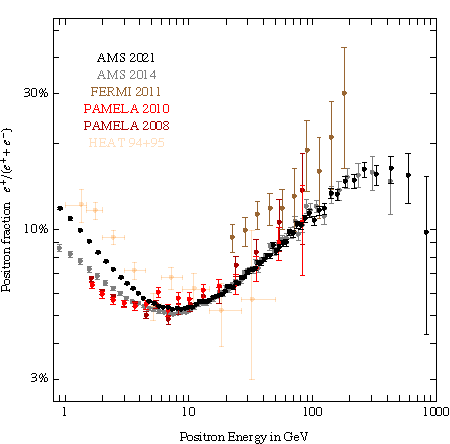
\includegraphics[width=0.48 \textwidth]{figs/CRdata_positron_fraction_2023} \quad
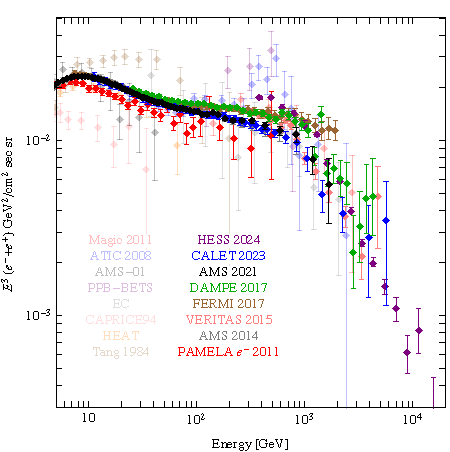
\includegraphics[width=0.48 \textwidth]{figs/CRdata_all_leptons_2024.pdf} \\
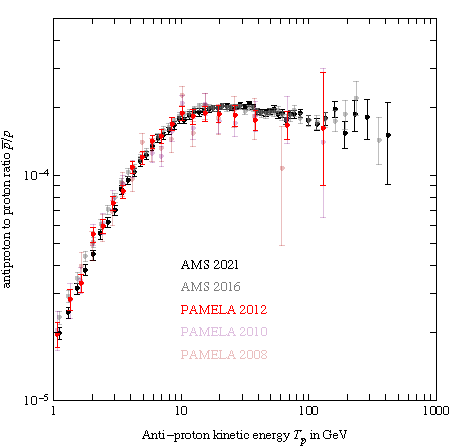
\includegraphics[width=0.48 \textwidth]{figs/CRdata_pbarratio} \quad
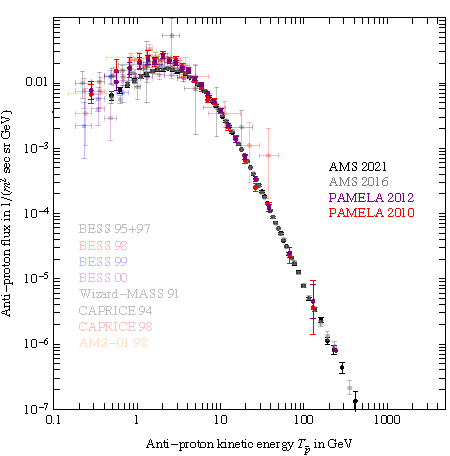
\includegraphics[width=0.48 \textwidth]{figs/CRdata_pbar.pdf} \\
\end{center}
\caption[Charged cosmic ray data.]{\em \small \label{fig:CRdata} A compilation of both historical and recent measurements of {\bfseries charged cosmic rays}, relevant for weak-scale DM indirect detection. Top left: positron fraction. Top right: electron and positron (`all lepton') flux. Bottom left: anti-proton to proton ratio. Bottom right: anti-proton flux. References are given in table \ref{tab:CRdatareferences}.} 
\end{figure}



\begin{itemize}
\item[$\circ$] {\em High-energy photons ($\gamma$-rays)} are observed using three main techniques. 
\begin{itemize}
\item Experiments in space (such as {\sc Fermi} or {\sc Ams-02}) detect $\gamma$-rays directly via pair conversions in the instrument. They scan the sky continuously and have typically a large field of view. 
\item Imaging atmospheric \v Cerenkov telescopes (IACT, such as {\sc Hess}, {\sc Magic}, {\sc Veritas} and the future {\sc Cta}) detect the \v Cerenkov light produced in the air by the shower of particles  when an energetic $\gamma$-ray collides with the top of the atmosphere.  They operate only on moonless clear nights and have to point in a narrow field of view. However, these ground-based experiments are sensitive to higher energies (typically around the TeV)
than space experiments (limited by the size of the instruments).
\item Air \v Cerenkov telescopes consist of large detectors situated on the ground, where they collect  particles from atmospheric cascades. {\sc Hawc} and {\sc Milagro}, for instance, consist of large tanks filled with water. They detect passing particles via the emitted \v Cerenkov radiation. They have almost continuous full sky view and are sensitive to very high energies, indicatively from TeV to PeV. 
\end{itemize}


\item[$\circ$] {\em Low-energy photons ($X$-rays, radio waves)} are detected by dedicated instruments. $X$-ray devices (such as {\sc Chandra}, {\sc Integral} or {\sc eRosita}) need to be deployed on balloons, rockets, or in space. For the purposes of DM searches they typically offer good spatial accuracy and exquisite energy resolution. Radio telescopes are ground-based instruments  and typically offer even better spatial resolution.

\item[$\circ$] {\em Charged cosmic rays (positrons, electrons, anti-protons)} are detected in space in a manner analogous to $\gamma$-rays. 
Using tracking and calorimetry, the detectors determine the identity of the particle and measure its energy. 
Tracking and calorimetry remain effective up to a certain maximal energy, largely dictated by the size of the apparatus, which, on the other hand, 
is limited by the fact  that the detector must be sent into space. 
Coupled with the fact that the fluxes at higher energies are suppressed, this explains why the spectra are measured only up to a certain
maximal energy, as shown in fig.\fig{CRdata}.
If the experiment is equipped with a magnet (like {\sc Pamela} or {\sc Ams}), it can distinguish between particle charges, allowing for differentiation between particles and antiparticles based on the unique curvature of their respective tracks.
This capability is crucial for DM searches because, generally, the astrophysical background of anti-particles is smaller than the one of particles. 
Experiments lacking a  magnet (like {\sc Calet} or {\sc Dampe}) are limited to measuring the total flux, e.g.,~$e^++e^-$. 
{\sc Fermi}, however, has been able to successfully use the magnetic field of the Earth for this purpose. 
Above about 1 TeV, the spectra of electrons and positrons have also been measured on Earth by the IACT detectors (such as {\sc Hess} and {\sc Veritas}).



\item[$\circ$] {\em Anti-deuterons (and heavier anti-nuclei)} are detected in space using methods similar to those for other charged particles: they can be differentiated from the much more abundant anti-protons, e.g.,~in {\sc Ams-02}, thanks to different charge-to-mass ratio. The dedicated balloon experiment {\sc Gaps} \cite{Gaps} aims to detect anti-deuterons employing a novel technique: the approach involves slowing down the $\bar{d}$ nucleus, capturing it within the detector to form an exotic atom, which then annihilates, emitting characteristic $X$-ray and pion radiation. Like previous balloon missions, {\sc Gaps} will be flown over Antarctica to maximize the signal --- low energy charged particles are deflected by the terrestrial magnetic field at lower latitudes. For a comprehensive overview see \cite{antideuteronssearches}.

\item[$\circ$] {\em Neutrinos} are detected using large \v Cerenkov detectors situated underground (or under-ice or under-water). The detection is via showers of secondary particles generated when neutrinos interact with the material inside the instrumented volume or its surroundings. 
Among these secondary particles, charged ones, in particular muons, emit \v Cerenkov light when traversing the detector and thus their energies and directions can be measured
(these are partially correlated with those of the parent neutrino). The main background for this search is due to the large flux of cosmic muons coming from the atmosphere above the detector. To mitigate this the experiments typically have to select only up-going tracks, i.e.,\ due to neutrinos that have crossed the entire Earth and interacted either within or just below the instrumented volume.
\end{itemize}




\subsection{Indirect detection: current constraints}
\label{sec:IDconstraints}
A large number of searches for DM annihilation or decay signals turned up empty handed. 
Therefore, these measurements merely set upper bounds on DM annihilation cross section or decay rate.
These limits are obtained by requiring that the flux from DM, possibly combined with the known or presumed astrophysical background, does not exceed the measured flux. 
Results are conveniently presented in the planes ($M$, $\langle \sigma v \rangle_{\rm ann}$) and  ($M$, $\tau$), where for annihilation (decay) the regions above (below) the limiting lines are ruled out.


\subsubsection{Constraints on DM with weak-scale mass}\label{sec:IDconstraintsWIMPs}
We first consider weak-scale DM, with a mass roughly in the range GeV to 100 TeV, which has been the focus of extensive searches in the past decades. 
Fig.~\ref{fig:IDconstraints} and \ref{fig:IDconstraintsdecay} provide a selection of the most relevant bounds, 
organized by DM annihilation channel and by SM messenger particle species. The CMB constraints are discussed in section~\ref{sec:cosmoconstraintsCMB} and the BBN ones in section~\ref{sec:BBNconstraints}.


For DM annihilations, the relevant benchmark is the thermal cross-section derived in eq.~(\ref{eq:sigmavcosmo}) and plotted in detail in fig.~\ref{fig:Omegafreeze-out} (left). As discussed in section \ref{sec:thermal_relic}, this cross-section corresponds to the annihilation rate that, within a large class of minimal models, 
reproduces the observed DM relic abundance through a thermal freeze-out process. 
In the case of decays, there is no analogous benchmark decay rate.

The annihilation constraints scale with the DM mass  roughly as $\langle \sigma v \rangle /M \approx$ constant (except the constraints on neutrino fluxes, see below). 
This scaling can be understood qualitatively: since the DM number abundance scales as $1/M$, 
the flux of annihilation products (charged cosmic rays or gamma rays) scales as $M^{-2}$, see~eq.~(\ref{gammaflux}). 
The total amount of injected products, on the other hand,  is proportional to $M$, since all the energy of the annihilated DM particles transforms into cosmic rays, 
hence the bound on $\langle \sigma v \rangle$ scales as $\propto M$. 
This scaling is well respected by the CMB constraints (see the discussion in section \ref{sec:cosmoconstraints}), for which the total energy injected in the DM annihilation is the only relevant parameter. For charged cosmic rays and gamma rays, the shape of the spectrum and the propagation effects also play a role, making the dependence on $M$ less pronounced.
For DM decay rates, the constraints remain constant with respect to $M$, because the flux of annihilation products scales as $M^{-1}$.


\begin{figure}[!t]
\begin{center}
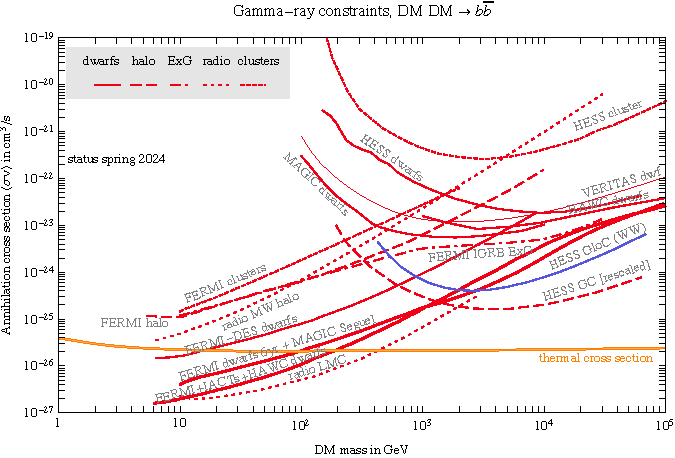
\includegraphics[width=0.80 \textwidth]{figs/ID_all_constraints_gammabb} 
\end{center}
\caption[Bounds from gamma rays]{\em\label{fig:IDconstraints_gammas} {\bfseries Bounds on weak-scale DM annihilations} 
imposed by different {\bfseries gamma-ray} (and radio) observations
assuming a typical hadronic DM annihilation channel, into $b\bar b$.
Certain constraints have been rescaled with respect to those published in the literature, in order to correct for the different choices of DM profiles: when possible, they have been brought to the standard NFW profile. 
The almost horizontal orange thin band is the thermal cross section of eq.~(\ref{eq:sigmavcosmo}), also plotted in fig.~\ref{fig:Omegafreeze-out} (left). 
We gratefully acknowledge the contribution of Alo\"ise Dijoux in compiling these results.}
\end{figure}

\begin{figure}[t]
\begin{center}
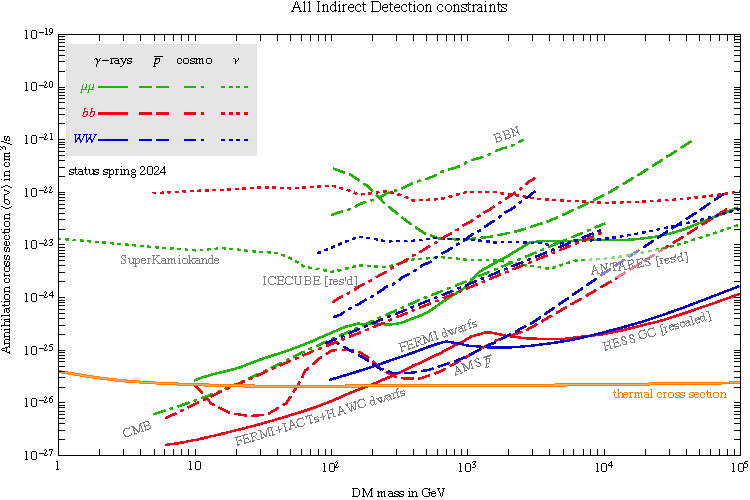
\includegraphics[width=0.80 \textwidth]{figs/ID_all_constraints} 
\end{center}
\caption[Bounds from all indirect detection channels]{\em \small \label{fig:IDconstraints} 
Summary chart of the {\bfseries current most stringent bounds on weak-scale DM annihilations}
into $\mu^+\mu^-$ (green),
$b\bar b$ (red) or $W^+W^-$ (blue),  from different searches, as discussed in the main text. 
Some constraints are rescaled with respect to the literature, to correct for the different choices of DM profiles.
The almost horizontal orange thin band is the thermal cross section of eq.~(\ref{eq:sigmavcosmo}), also plotted in fig.~\ref{fig:Omegafreeze-out} (left).}
\end{figure}




\begin{figure}[p]
\begin{center}
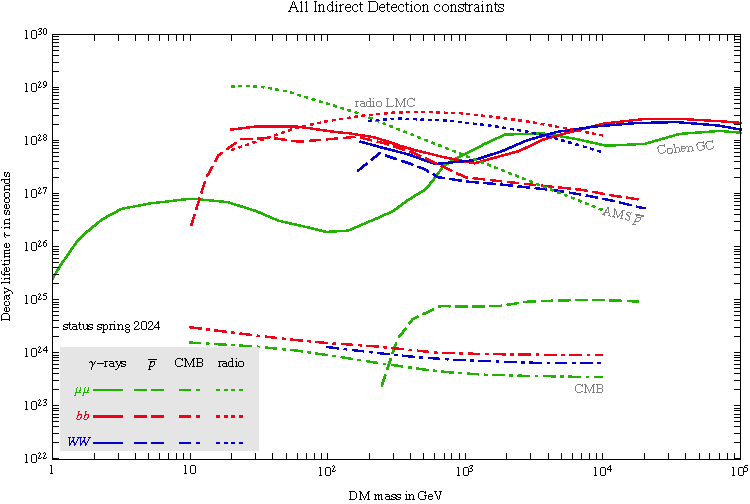
\includegraphics[width=0.80 \textwidth]{figs/ID_all_constraints_decay} 
\end{center}
\caption[Bounds from all indirect detection channels (decay case)]{\em \small \label{fig:IDconstraintsdecay} Summary plot of the {\bfseries most stringent current bounds on decaying weak-scale DM}, in different channels and from different searches, as discussed in the main text.}
\end{figure}



\begin{table}[p]
\resizebox{\columnwidth}{!}{
\begin{tabular}{|l||c|c|c|c|c|c|}
\hline \rowcolor[rgb]{0.95,0.97,0.97}
 & {\bf GC / GCH} & {\bf MW halo} & {\bf Dwarfs} & {\bf Clusters} & {\bf Cosmological} & {\bf other} \\
\hline
\multicolumn{7}{c}{} \\
\multicolumn{7}{c}{\bf DM annihilation: $\mb{\gamma}$-ray searches } \\
 \hline
{\multirow{6}{*}{\rotatebox[origin=c]{90}{\bf ~~~~~~ continuum }}} & {\sc Hess}~\cite{Abramowski:2011hc,Lefranc:2015vza,1607.08142,2207.10471} & {\sc Fermi}~\cite{Ackermann:2012rg} & {\sc Magic}~\cite{Aleksic:2013xea,MAGIC:2017avy,MAGIC:2020ceg} & {\sc Fermi}~\cite{Ackermann:2010rg,Ackermann:2015fdi,Thorpe-Morgan:2020czg} & {\sc Fermi}~\cite{Ackermann:2015tah} & {\sc Fermi}~\cite{Ackermann:2012nb} \\
 & ({\sc Fermi}~\cite{TheFermi-LAT:2015kwa}) & {\sc Hawc}~\cite{HAWC:2017udy,HAWC:2023owv} & {\sc Hess}~\cite{Abramowski:2014tra,HESS:2020zwn} & {\sc Hess}~\cite{Abramowski:2012au} & & {\footnotesize (dark satellites)} \\\cline{7-7}
 & Abazajian et al.~\cite{2003.10416} &  & {\sc Fermi}~\cite{Ackermann:2015zua} & {\sc Veritas}~\cite{Pfrommer:2012mm} & &  {\sc Hess}~\cite{Abramowski:2011hh} \\ 
 & & & {\sc Fermi}+{\sc Magic}~\cite{Ahnen:2016qkx} & & & {\footnotesize (GloCs)} \\ \cline{7-7}
 & & & {\sc Fermi-Des}~\cite{Drlica-Wagner:2015xua} & & &  {\sc Veritas}~\cite{NietoCastano}  \\ 
 & & & {\sc Hawc}~\cite{Albert:2017vtb} & & & {\footnotesize (subhalos) }\\  
 & & & {\sc Veritas}~\cite{1703.04937} & & & \\
 & & & {\sc Fermi}+{\sc Iact}s+& & & \\
 & & & +{\sc Hawc}\cite{Hess:2021cdp} & & & \\
 & & & McDaniel et al.~\cite{McDaniel:2023bju} & & & \\
\hline
{\multirow{2}{*}{\rotatebox[origin=c]{90}{\bf \hspace{3ex}lines }}} & {\sc Hess}~\cite{Abramowski:2013ax,1609.08091,1805.05741} & {\sc Fermi}~\cite{Ackermann:2015lka} & {\sc Magic}~\cite{Aleksic:2013xea} & {\sc Fermi}~\cite{Anderson:2015dpc,Thorpe-Morgan:2020czg}& & \\
 & & & {\sc Hess}~\cite{HESS:2018kom,HESS:2020zwn} & & & \\
 & & & {\sc Veritas}~\cite{1703.04937} & & & \\
  & & & {\sc Hawc}~\cite{HAWC:2019jvm} & & & \\
 \hline
\multicolumn{7}{l}{  } \\
\multicolumn{7}{c}{\bf DM annihilation: neutrino searches } \\
\hline
{\multirow{4}{*}{\rotatebox[origin=c]{90}{\bf \hspace{4ex}continuum }}} & {\sc Antares}~\cite{1505.04866,1912.05296,ANTARES_ICRC2023} & {\sc Icecube}~\cite{1406.6868,1606.00209,2303.13663} & {\sc Icecube}~\cite{1307.3473,1510.05226,2511.19385} & {\sc Icecube}~\cite{1510.05226}  &  &  \\
 & {\sc Icecube}~\cite{1505.07259,1705.08103} & {\sc Antares}~\cite{1612.04595} & {\sc Baikal}~\cite{1612.03836} & & & \\  
 & {\sc SuperK}~\cite{1510.07999,2005.05109} & & & & & \\
 & {\sc Baikal}~\cite{1512.01198} & & & & & \\
 & {\sc Antares+} & & & & & \\
 & {\sc Icecube}~\cite{2003.06614} & & & & & \\
 & {\sc Antares} (heavy/& & & & & \\
 & secluded DM)~\cite{2203.06029} & & & & & \\
 \hline
{\multirow{4}{*}{\rotatebox[origin=c]{90}{\bf lines  }}} & {\sc Antares}~\cite{1612.04595,ANTARES_ICRC2023} & {\sc Icecube}~\cite{1406.6868,1606.00209,2303.13663}  & {\sc Icecube}~\cite{1307.3473,1510.05226,2511.19385}  & & & \\
  & {\sc Icecube}~\cite{1505.07259,1705.08103} &  & {\sc Baikal}~\cite{1612.03836} & & & \\ 
  & {\sc SuperK}~\cite{1510.07999,2005.05109} & & & & & \\
   & {\sc Baikal}~\cite{1512.01198} & & & & & \\[1ex]
\hline
\multicolumn{7}{l}{  } \\
\multicolumn{7}{c}{\bf DM decay: $\mb{\gamma}$-ray searches } \\
\hline 
{\multirow{5}{*}{\rotatebox[origin=c]{90}{\bf continuum }}} &  &  &  &  &  &  \\
 & Cohen et al. \cite{1612.05638} &  {\sc Fermi}~\cite{Ackermann:2012rg} & {\sc Veritas}~\cite{1202.2144} & {\sc Fermi}~\cite{1110.6863} & Cirelli et al.~\cite{1205.5283} &  \\
 & Esmaili et al.~\cite{Esmaili:2021yaw} & {\sc Hawc}~\cite{HAWC:2017udy,HAWC:2023owv} & {\sc Magic}~\cite{Aleksic:2013xea} &  {\sc Magic}~\cite{MAGIC:2018tuz} & &  \\
 &  & & {\sc Hawc}~\cite{1706.01277} & {\sc Hawc}~\cite{Albert:2023ucd} & &  \\
 &  & &  &  & &  \\
 \hline
\rotatebox[origin=c]{90}{\bf  \ lines } & & {\sc Fermi}~\cite{Ackermann:2015lka} & {\sc Magic}~\cite{Aleksic:2013xea}  & & & \\
\hline
\multicolumn{7}{l}{  } \\
\multicolumn{7}{c}{{\bf DM decay: neutrino searches:} {\sc Icecube}~\cite{1101.3349,1804.03848,2107.11527,2303.13663}}
\end{tabular}
}


\caption[Main indirect detection searches]{\label{tab:gammanuconstraints} \em A collection of the currently most relevant  {\bfseries $\mb{\gamma}$-ray and neutrino searches for weak-scale DM}, as produced by different (mostly experimental) collaborations. The top tables pertain to the annihilating DM, the bottom one to decaying DM. The targets correspond to the broad classification presented in section~\ref{sec:IDgamma}.}
\end{table}





\begin{table}
\setlength\tabcolsep{10pt} \renewcommand{\arraystretch}{1.6}
\scriptsize{
\begin{center}
\begin{tabular}{|p{0.19\textwidth}|p{0.60\textwidth}|}
\hline
{\bf CR species} & {\bf Experiments}  \\
\hline
\hline
Positron fraction \newline $e^+/(e^++e^-)$  & {\sc Heat} 1997 \cite{Barwick:1997ig} $-$ {\sc Pamela} 2008 \cite{Adriani:2008zr} $-$ {\sc Pamela} 2010 \cite{Adriani:2010ib} $-$ {\sc Fermi} 2011 \cite{FermiLAT:2011ab}  $-$ {\sc Ams} 2013 \cite{AMSpositrons2013} $-$ {\sc Pamela} 2013 \cite{Adriani:2013uda} $-$ {\sc Ams} 2014 \cite{AMSpositrons2014} $-$ {\sc Ams} 2019 \cite{AMSele2019} \\
\hline
All leptons \newline ($e^++e^-$)        &  {\sc Hess} 2009 \cite{HESSleptons} $-$ {\sc Fermi} 2010 \cite{FERMIleptons} $-$ {\sc Magic} 2011 \cite{BorlaTridon:2011dk} $-$ {\sc Ams} 2014 \cite{Aguilar:2014fea} $-$ {\sc Voyager1} 2015 \cite{Voyagerepem} $-$ {\sc Veritas} 2015 \cite{Staszak:2015kza} $-$ {\sc Fermi} 2017 \cite{Abdollahi:2017nat} $-$ {\sc Hess} 2017 \cite{HESSleptons2017prelim} $-$ {\sc Dampe} 2017 \cite{DAMPEepem} $-$ {\sc Calet} 2017 \cite{CALETepem} $-$ {\sc Calet} 2018 \cite{Adriani:2018ktz} $-$ {\sc Veritas} 2018 \cite{VERITAS:2018iqb} $-$ {\sc Ams} 2019 \cite{AMSele2019} $-$ {\sc Ams} 2021 \cite{Aguilar:2021tos} $-$ {\sc Calet} 2023 \cite{CALET:2023emo}  $-$ {\sc Hess} 2024 \cite{HESS:2024etj}  \\ 
\hline
Positrons \newline $e^+$ 		&  {\sc Fermi} 2011 \cite{FermiLAT:2011ab} $-$  {\sc Pamela} 2013 \cite{Adriani:2013uda} $-$ {\sc Ams} 2014 \cite{AMSepem2014} $-$  {\sc Ams} 2018 \cite{Aguilar:2018ons} $-$ {\sc Ams} 2019 \cite{AMSpos2019} \\
\hline
Electrons \newline $e^-$		& {\sc Pamela} 2011 \cite{Adriani:2011xv} $-$ {\sc Fermi} 2011 \cite{FermiLAT:2011ab} $-$ {\sc Ams} 2014 \cite{AMSepem2014} $-$  {\sc Ams} 2018 \cite{Aguilar:2018ons} $-$  {\sc Ams} 2019 \cite{AMSele2019} \\
\hline
anti-proton/proton ratio \newline $\bar p/p$ & {\sc Pamela} 2008/10/12 \cite{PAMELApbar} $-$ {\sc Argo-ybj} 2012 \cite{Bartoli:2012qe}  $-$  {\sc Ams} 2016 \cite{Aguilar:2016kjl} \\ 
\hline
anti-protons \newline $\bar p$ 		& {\sc Wizard-Mass} 1991 \cite{Basini:1999hh} $-$ {\sc Caprice} 1994 \cite{Boezio:1997ec} $-$ {\sc Bess} 1996-97 \cite{Orito:1999re} $-$ {\sc Bess} 1998 \cite{Maeno:2000qx} $-$  {\sc Caprice} 1999 \cite{Boezio:2001ac} $-$ {\sc Bess} 1999-2000 \cite{Asaoka:2001fv} $-$ {\sc Ams01} 2001 \cite{Aguilar:2002ad} $-$ {\sc Pamela} 2010/12 \cite{PAMELApbar} $-$ {\sc Bess} 2012 \cite{Abe:2011nx} $-$ {\sc Ams} 2016 \cite{Aguilar:2016kjl} $-$ {\sc Ams} 2021 \cite{Aguilar:2021tos} \\
\hline
Protons \newline $p$ 			& {\sc Pamela} 2011 \cite{Adriani:2011cu} $-$ {\sc Voyager1} 2015 \cite{Voyagerepem} $-$ {\sc Ams} 2015 \cite{Aguilar:2015ooa} $-$ {\sc Calet} 2019 \cite{Adriani:2019aft} $-$ {\sc Dampe} 2019 \cite{An:2019wcw} $-$ {\sc Ams} 2021 \cite{Aguilar:2021tos} \\
\hline
Antideuterons \newline $\bar d$   		&  {\sc Bess} 2005 \cite{Fuke:2005it} $-$ {\sc Bess-Polar II} 2023 \cite{Sakai:2023uka} \\ 
\hline
Antihelium \newline $\overbar{He}$   		&  {\sc Ams-01} 1999 \cite{AMS:1999tha} $-$ {\sc Pamela} 2011 \cite{Mayorov:2011zz} $-$ {\sc Bess-Polar II} 2012 \cite{Abe:2012tz} \\ 
\hline
\end{tabular}
\end{center}}
\caption[Recent charged CR data]{\em  {\bfseries Recent data on charged cosmic rays} with relevance for weak-scale DM indirect detection. An exhaustive list of data can be found on the \href{https://lpsc.in2p3.fr/crdb}{Cosmic-Ray database}~\cite{CRDB}. 
\label{tab:CRdatareferences}}
\end{table}

\medskip

{\bf Gamma-rays}. Gamma-ray searches for DM signals have been pursued since the very beginning of indirect detection, in a variety of targets and energy ranges. 
In table \ref{tab:gammanuconstraints} we list the main (negative) results, both for DM annihilations and decays. For brevity, we focus mostly on the `official' results from the experimental collaborations rather than on the works by independent groups of theorists. 
A selection of the bounds is reproduced in fig.~\ref{fig:IDconstraints_gammas}.\footnote{For a recent exhaustive list of searches see also 
\arxivref{2208.00145}{H\"utten and Kerszberg (2022)} in \cite{otherpastDMreviews}.} Note that some of the constraints have been rescaled  from their originally published values, in order to correct for the different choices of DM profiles: when possible, they have been brought to the standard NFW profile.

For DM masses up to about 1 TeV the most stringent constraints come from dwarf galaxies.  For heavier DM, the constraints derived from {\sc Iact} observations of the GC, notably {\sc Hess}, take over. 


\smallskip

{\bf Radio-waves}. Radio observations have long been employed to set constraints on the synchrotron emissions from DM  \cite{DMradiobounds}. 
Historically, observations focused on small regions near the GC, since the expected large DM density and the presence of a strong magnetic field  
guarantee significant emissions  in this region.
However, uncertainties are also largest around the GC, both regarding the DM distribution, the astrophysical environments and the background emissions. 
Later on, several studies shifted the focus to much larger regions  of the galactic halo (or even the whole galactic halo), which can provide more robust results. 
Outer galaxies and galaxy clusters have also been considered, as well as isotropic signals of extragalactic origin. In fig.s~\ref{fig:IDconstraints_gammas}, \ref{fig:IDconstraints} and \ref{fig:IDconstraintsdecay}, we report a few selected bounds, selecting the most conservative estimates. 
Notably, the recent constraints derived in \arxivref{2106.08025}{Regis et al.~(2021)} \cite{DMradiobounds} from observations of the Large Magellanic Cloud, if confirmed, are very stringent. 

\arxivref{2204.04232}{Manconi et al.~(2022)} \cite{DMradiobounds} considered the {\em polarization} of the radio-waves emitted by $e^+e^-$ from DM annihilations, while these gyrated in the galactic magnetic field, and compared it with the polarization maps produced by {\sc Planck}. 
This results in stringent constraints on leptonic DM annihilation channels, 
however, assumptions regarding the galactic magnetic field can change the results by approximately  an order of magnitude.


\smallskip

{\bf Anti-protons (and electrons or positrons)}. Measurements of charged cosmic rays, a compilation of which is given in figure \ref{fig:CRdata} and table \ref{tab:CRdatareferences}, can also be used to impose competitive constraints. 
The anti-proton bounds reported in fig.~\ref{fig:IDconstraints} and \ref{fig:IDconstraintsdecay} were derived in~\cite{Calore:2022stf}. 
They are based on the 2016 results of {\sc Ams-02}, but do not change significantly if the 2021 data are used instead. The reported bounds are significantly more stringent than previous constraints~\cite{Giesen:2015ufa} for DM masses larger than 200 GeV and less stringent for lower DM masses. Notably, some authors have recently identified a possible excess at low DM masses in the same data, as discussed in section~\ref{sec:pbarexcess}. 

Some authors have also derived bounds from electrons or positrons (not reported in the figure) \cite{epconstraints}. Given that these channels exhibit clear excesses (see section \ref{sec:positronexcess}), the strategy is to attribute these excesses to astrophysical sources, and then search for any additional features in the spectrua that would be produced by DM. This strategy is possible for DM annihilating or decaying into a leptonic channel, since this produces a distinctive sharp feature.

\smallskip

{\bf Anti-deuterons}. The only current upper bound on the flux of cosmic anti-deuterons comes from the {\sc Bess} experiment \cite{Fuke:2005it,Sakai:2023uka} and is too weak to give any significant constraints on annihilating or decaying DM. The planned sensitivities of {\sc Ams} and {\sc Gaps}, though, may allow to test interesting regions of the DM parameter space,  for 100 GeV DM even down to the thermal cross section, in optimal conditions \cite{antiD,antideuteronssearches,antiDprospects}. 
An advantage of anti-deuteron searches is that the astrophysical background and DM signal peak at different energy ranges. Specifically, while the astrophysical background typically peaks at a few GeV per nucleon, the DM signal is expected to peak at energies below 1 GeV/n,  so that the search for a DM $\bar d$ signal can be considered as essentially background-free. 
The underlying reason is that the astrophysical $\bar d$ are produced in spallation of high-energy cosmic rays on the interstellar gas: the kinematics is such that low energy $\bar d$ are produced only very rarely. The DM $\bar d$'s are, in contrast, produced from a coalescence of $\bar p$ and $\bar n$ from essentially-at-rest DM particles and are not subject to the same kinematical constraints. For a recent detailed discussions of the light anti-nuclei astrophysical backgrounds see \cite{antinucleibkg}. 

\smallskip

{\bf Anti-helium}. Upper bounds on the flux of cosmic anti-helium nuclei come from {\sc Ams-01}~\cite{AMS:1999tha}, {\sc Pamela}~\cite{Mayorov:2011zz} and {\sc Bess-Polar II}~\cite{Abe:2012tz}. They are much higher that than the flux predicted by DM and by astrophysics. See however the detailed discussion in section~\ref{sec:antiHeexcess} concerning a possible anomaly in this channel.

\smallskip

{\bf Neutrinos}. All current experiments ({\sc Icecube}, {\sc Antares}, {\sc SuperKamiokande} and {\sc Baikal}) impose constraints from the non-observation of high-energy neutrino fluxes from the Galactic Halo and Galactic Center. References for these experiments can be found in table \ref{tab:gammanuconstraints}, and the most significant bounds are depicted in fig.s~\ref{fig:IDconstraints} and \ref{fig:IDconstraintsdecay}.\footnote{The combined {\sc Antares + Icecube} limits in \cite{2003.06614} are more stringent than the individual ones. However, they span only a limited range of DM masses, 
so they are not reported in the figure.} 
Quantitatively, the constraints derived from neutrino flux are somewhat weaker  than the $\gamma$-ray bounds discussed above (both in the case of DM annihilation and decay).  
Nevertheless, they offer an advantage:  they are less dependent on the DM particle mass.
This is because neutrino cross sections grow with energy, so that the higher energy neutrinos coming from annihilations of heavier DM have a higher probability for detection in the material of a neutrino telescope, which partly compensates for the reduced flux.
Neutrino constraints, both for annihilation and decay, are competitive with $\gamma$-ray constraints for DM masses above several TeV. 
\arxivref{1912.09486}{Arguelles et al.~(2019)} \cite{Arguelles:2019ouk} compiled current bounds and future sensitivities also for very small and very large DM masses.
A robust upper bound on the total annihilation cross-section, of the order of $\sigma v_{\rm rel} \circa{<} 10^{-21}\cm^3/\sec$ for $1 \ {\rm GeV} \lesssim M \lesssim 100$ TeV, can be imposed focusing on the least detectable messengers, namely neutrinos, and comparing the predicted flux with the atmospheric neutrino measurements \cite{ultimateannbound}.

\smallskip

{\bf Invisible radiation}.
The weakest bounds arise if DM annihilates or decays into invisible radiation, such as gravitons or  hypothetical extra particles much lighter than $M/2$.
The bound on the DM lifetime is~\cite{DMinvisibleDecay}
\beq \tau/f  \gtrsim 250 \,{\rm Gyr}, 
\eeq
where the factor $f\le 1$ accounts for the possibility that only a fraction $f$ of DM decays into invisible relativistic particles (this decaying component of DM has a life-time $\tau$). 
The above bound implies that up to today at most $\approx 5\%$ of DM decayed or annihilated in this way.
% 2% if tau << T_U


\smallskip

{\bf Other constraints}. 
The observation of the absorption of 21cm radiation by the {\sc Edges} experiment  (see section~\ref{sec:EDGESanomaly}) can be used to derive constraints on both annihilating and decaying DM~\cite{EDGESbounds}.


Another strategy used to set bounds on annihilating or decaying DM
are the cross-correlations among different sources or signals
discussed in section \ref{sec:correlations}.
For annihilating DM, the cross-correlations exclude the thermal cross-section for  DM with mass below
$M\circa{<}20\GeV$, in specific configurations (see e.g.~\cite{crosscorrelations}). These constraints are an order of magnitude weaker than the most stringent bounds from other strategies discussed above. 
For decaying DM, the decay times of roughly $10^{-25-26}/\rm{s}$ are excluded, 
which is also much weaker than the bounds obtained using other probes. 
The projected future sensitivities of cross-correlations are, however, quite promising, possibly reaching the thermal cross-section for TeV DM, in ideal configurations.


\medskip

The rough overall result is that indirect detection implies $\sigma v_{\rm rel} \circa{<} 10^{-27-24}\cm^3/\sec$, depending on the DM
mass and annihilation channel. In some cases this excludes the thermal cross section, e.g.,\ for DM lighter than $\sim 200\GeV$ annihilating
into $b\bar b$ quarks. 
Assuming that DM annihilates into a generic visibile channel implies the lower limit $M \gtrsim 20\GeV$, 
obtained in \arxivref{1805.10305}{Leane et al.~(2018)}~\cite{1805.10305} by marginalizing over the branching ratios.
Bounds on the DM lifetime are at the $\tau\circa{>} 10^{27-28}$seconds level, about 10 orders of magnitude longer than the age of the Universe.

\begin{figure}[t]
\begin{center}
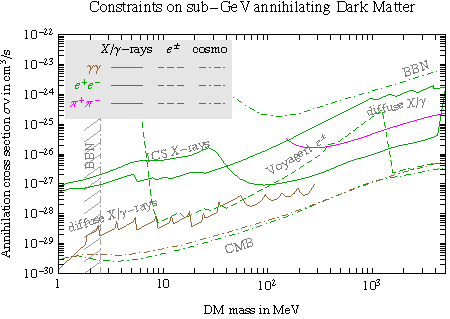
\includegraphics[width=0.48 \textwidth]{figs/ID_subGeV.pdf} \quad
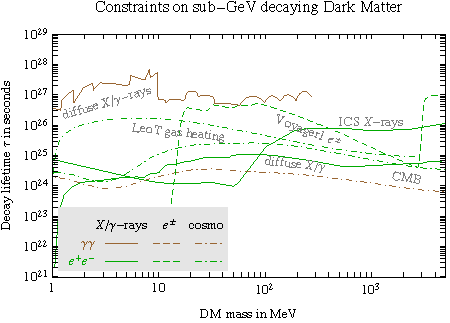
\includegraphics[width=0.48 \textwidth]{figs/ID_subGeV_decay.pdf} 
\end{center}
\caption[Indirect detection bounds on sub-GeV DM]{\em\label{fig:IDconstraintssubGeV} Summary plots 
of the current {\bfseries bounds on sub-GeV DM} annihilations (left) or decays (right)
from different searches, as discussed in the main text.}
\end{figure}


\subsubsection{Constraints on sub-GeV DM}\label{sec:IDconstraintsSub-GeV}
Next, let us consider DM with roughly MeV to GeV mass. 
The indirect detection constraints for this mass range are reported in figure~\ref{fig:IDconstraintssubGeV} ~\cite{subGeVconstraints}. The kinematically allowed annihilation or decay channels are: $\gamma \gamma$, neutrinos, $e^+e^-$, $\mu^+\mu^-$. One can also consider DM annihilations or decays into quarks, producing $\pi^+\pi^-$ and $\pi^0\pi^0$. If DM is heavier than a few GeV, it can also produce $p\bar p$ pairs. 

\smallskip 


The basic principles and techniques for indirect searches in this mass range are the same as for weak-scale DM, discussed above. 
However, certain unique characteristics do exist:
\begin{itemize}
\item[$-$]
 Regarding charged particles (primarily $e^\pm$ and potentially $\bar p$): particles with sub-GeV energies are not able to penetrate the heliosphere and therefore cannot  be detected by detectors located in the Earth's orbit.  Currently, only the {\sc Voyager-}1 and -2 space probes have crossed the outer boundary of the heliosphere, and are thus uniquely positioned to search for these signals. 

\item[$-$]
The MeV to GeV photons (i.e., the hard $X$-rays and soft $\gamma$-rays) are in principle a powerful tool, however, there are only a few current telescopes with good sensitivities and acceptances in this energy range (see the list in table \ref{tab:IDexp}). At energies below a few MeV, {\sc Integral} and {\sc Chandra} can be used. At energies above 100 MeV {\sc Fermi-Lat} takes over. In between, only the relatively old telescope {\sc Comptel} is relevant. A number of different experiments are being proposed to fill this so-called \index{MeV gap} {\em MeV gap}. 
An alternative approach is to look for secondary emissions: if sub-GeV DM annihilates or decays into channels that contain $e^\pm$, these produce inverse Compton photons in the $X$-ray energy range (see section \ref{sec:ICS}), which can be tested with telescopes such as {\sc Integral} and {\sc eRosita}. Currently, this actually produces some of the most stringent  constraints.\footnote{In the same vein, let us mention that the synchrotron  secondary emission from $e^\pm$ around super-massive black holes can lead to even more stringent constraints, however under significant assumptions for the magnetic field and the DM distribution (see \arxivref{2404.16673}{Chen et al.~(2024)} in \cite{subGeVconstraints}).}  

\item[$-$]
DM neutrinos with MeV energies are typically overwhelmed by the solar and atmospheric neutrino backgrounds. 

\item[$-$]
The cosmological bounds remain relevant in the entire DM mass range. For annihilating DM the CMB constraints are among the most stringent ones. For decaying DM, there are relevant constraints for low DM masses which arise from requiring that there is no excessive heating in the gas-rich dwarf galaxy Leo T. For annihilating DM, the BBN bounds discussed in section \ref{sec:BBNconstraints} exclude a portion of the parameter space at small mass and another portion at large cross sections.
\end{itemize}

\subsubsection{Constraints on DM with mass above 100 TeV}\label{sec:IDconstraints100-TeV}
Let us briefly discuss super-heavy DM, characterized by
$M \gtrsim 100$ TeV. 
Such a large mass for annihilating DM requires a special mechanism to avoid the unitarity constraints discussed in section \ref{unitarity}. For this reason most of the bounds in the literature focus on the decaying DM case.
Model-independent constraints have been derived by the {\sc Hawc} \cite{HAWC:2017udy,HAWC:2023owv,Albert:2023ucd}, {\sc Magic} \cite{MAGIC:2018tuz} and {\sc Lhaaso} \cite{Cao:2022myt} collaborations, and by a number of independent groups \cite{Kalashev:2016cre,1612.05638,Kachelriess:2018rty,Ishiwata:2019aet,Esmaili:2021yaw,Chianese:2021jke} using data from other high-energy cosmic ray observatories such as {\sc Kascade}, {\sc Kascade-Grande}, {\sc Pao} (Pierre-Auger-Observatory), {\sc Ta} (Telescope Array), {\sc Casa-Mia}, {\sc Tibet-AS$\gamma$} as well as {\sc Icecube}.  
The {\sc Pao} collaboration derived constraints on a specific scenario of super-heavy decaying DM coupled to ultralight sterile neutrinos \cite{PierreAuger:2023vql}. 
The bounds on the DM lifetime reach $\tau\circa{>} 10^{29-30}\sec$, which is somewhat higher than for weak-scale DM.
The {\sc Hawc} \cite{HAWC:2017udy,Acharyya:2023ptu,HAWC:2023owv} collaboration also derived constraints on annihilating super-heavy DM.\footnote{For sensitivity estimates to annihilating super-heavy DM, see also \cite{Tak:2022vkb}.}
  


\section{Astrophysical searches for ultra-light DM}\label{sec:UDM:indirect}\index{Fuzzy DM}
As discussed in section~\ref{LightBosonDM}, DM could be a sub-eV boson, behaving as a classical oscillating field. 
On galactic and stellar scales, such light and ultra-light DM can exhibit unique phenomena, 
providing opportunities to probe and restrict its properties. 
 The discussion of indirect detection constraints on light DM, focusing on axions and axion-like particles, is covered in section \ref{AxionExp}. 
In this section, we focus on the phenomenology primarily associated with ultra-light (fuzzy) DM, 
which exhibits the following features~\cite{FuzzyDMbounds}:
\begin{itemize}
\item[$\circ$] 
Numerical simulations find that the {\bf DM density distributions} exhibit a {\bf core} 
at the centers of galaxies and dwarf galaxies (these cores are often referred to as `solitonic', meaning that their sizes are comparable to the DM wavelength). 
Outside the cores, DM density transitions to the NFW profile. 
One can show (see \arxivref{1805.00122}{N. Bar et al.~(2018)} in \cite{FuzzyDMbounds}) that in this case the circular velocities of the {\em inner} stars (within the core) are expected to be comparable to the circular velocities of the {\em outer} stars. This is not seen in observations, which rather find that the inner stars have smaller circular velocities.
Using this observational data one can place a bound  on DM mass, though a rather weak one, $M \gtrsim 10^{-21}$ eV, which is already the minimum DM mass compatible with the dwarf galaxy sizes, see eq.~(\ref{eq:DMmassrange}). 

If the dwarf galaxies do have cores, their masses $M_c$ are expected to scale with the masses of the galactic halos 
as $M_c\propto M_{\rm halo}^{\alpha}$, where $\alpha$ is typically found to be 1/3 but reaches $\sim 5/9$ in some studies~\cite{FuzzyDMbounds}. 
This predicts for dwarf satellite galaxies to have cores of kpc sizes  and masses of $\sim 10^8M_\odot$, which is in the right ballpark to potentially solve the small scale controversies in the cold DM model (see section \ref{sec:astroanomaly}).


\item[$\circ$] {\bf Interference} between different modes of the scalar field results in temporally transient {\bf density fluctuations} roughly the size of the DM wavelength. The interference can be constructive or destructive, so that the fluctuations can exhibit as either significantly over-dense or under-dense regions.\footnote{While fuzzy DM leads to the suppression of small-scale structures on cosmological scales due to quantum pressure (see section~\ref{LightBosonDM}), the interference  can create sharp structures on very small scales.}
For example, in regions where the field amplitude vanishes,
$\psi=0$, this defines 1-dimensional curves in space, approximately one per de Broglie volume.
This phenomenon can be probed via gravitational lensing. 
In fact, the study by \arxivref{2304.09895}{Amruth et al.~(2023)} in \cite{FuzzyDMbounds} contends that wave DM with a particle mass of  $M \sim 10^{-22}\, \eV$ provides a superior fit to a specific strong-lensing observation when compared to a particle DM NFW profile.\index{Ultra-light DM!strong lensing}
The phenomenon can also be probed via pulsar timing, since fluctuating gravitational potentials may oscillate at frequencies comparable to those of  pulsars, allowing for sensitive probes. 


These fluctuations in the gravitational potential can furthermore heat up the random motions of stars and disrupt tight conglomerations of stars such as the globular clusters. 
Using observations of 
globular clusters within the Eridanus II dSph galaxy, \arxivref{1810.08543}{Marsh and Niemayer~(2019)} in~\cite{FuzzyDMbounds} derived a constraint $M > 10^{-19}$ eV. 
The stellar heating can also lead to thicker galactic disks, possibly improving the agreement with observations for fuzzy DM with $M \sim 10^{-22}$ eV~\cite{FuzzyDMbounds}, which is, however, in some tension with the other bounds discussed in this section.

\item[$\circ$] One expects {\bf fewer sub-halos}, since `quantum pressure' can favour their disruption beyond the usual effects of tidal forces. Comparing with, e.g., the census of MW satellites, this imposes $M > 2.9~10^{-21}$ eV.


\item[$\circ$] {\bf Reduced dynamical friction} \index{Dynamical friction} is expected.
As discussed in section \ref{sec:DynamicalFriction}, a massive object moving through DM attracts DM, which then tends to form a slightly over-dense DM trail behind the object.
The gravitational pull on the object from the over-density in the trail creates a friction-like force.
This effect of dynamical friction is reduced  by fuzziness, possibly by up to an order of magnitude,
especially in systems with low DM velocities,
because then the de Broglie wave-length 
is larger.
If DM is ultra-light ($M \sim 10^{-22}$ eV, somewhat below the lower bound in eq.~(\ref{eq:DMmassrange})), 
this could help explain the survival of globular clusters outside galaxies. 


\item[$\circ$] Fuzzy DM could form soliton-like objects, known as
`{\bf bose stars}', with mass $m$ and size $R$ such that the `quantum pressure' balances the gravitational pull,
$G m/R\sim 1/M^2 R^2$, giving for the bose star radius, $R \sim M_{\rm Pl}^2/m M^2$ (see section \ref{sec:axionstar} for further details).
If $m\gtrsim M_{\rm Pl}^2/M \sim M_\odot (10^{-10}\eV/M)$ the system collapses into a black hole, since then
$R_{\rm Sch} \sim G m \circa{>}R$. 
Self-interactions modify the picture:
a negative scalar quartic coupling $\lambda_4<0$ (see eq.~(\ref{eq:Vwave})) causes an instability, resulting in a collapse, $R\to 0$,
such that relativistic effects become important.



\end{itemize}
In summary, while above effects do set bounds on fuzzy DM, subject to astrophysical uncertainties, they only restrict the lower end of the possible mass spectrum: $M \gtrsim 3~10^{-21}$ eV, 
if the Eridanus II cluster disruption bound is neglected, $M \gtrsim 10^{-19}$ eV, if it is included. In addition, black hole super-radiance, discussed below, can probe a wide range of larger fuzzy DM masses. 

\begin{figure}[t]
$$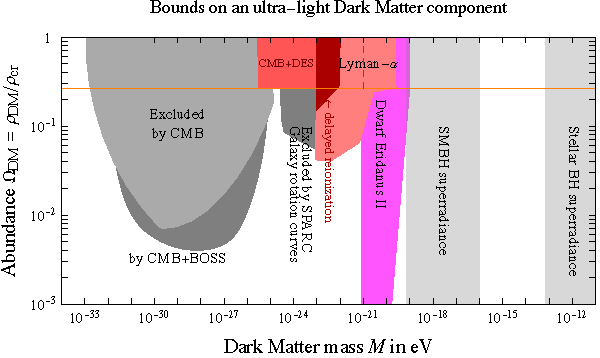
\includegraphics[width=0.70\textwidth]{figs/UltraLightDMexclusion}$$
\caption[Macroscopic DM]{\label{fig:ULDM}\em Bounds on the {\bfseries cosmological abundance of an ultra-light (fuzzy) DM component}. 
Figure adapted from fig.~3 of~\arxivref{2203.14915}{Antypas et al.~(2022)}~\cite{FuzzyDM}. References are listed  in \cite{FuzzyDMbounds2} and \cite{FuzzyDMbounds}. The figure somewhat naturally connects to fig.~\ref{fig:axion}, where the astrophysical, cosmological and laboratory constraints on axions and axion-like Dark Matter are presented. The vertical dashed  grey line signals the minimal DM mass of eq.~(\ref{eq:DMmassrange}). Laboratory constraints on ultra-light DM are discussed in section \ref{sec:UDM:direct}.} 
\end{figure}

\medskip


A wider parameter space opens up, if one relaxes the requirement that the fuzzy substance constitutes all of DM. Bounds that apply in this case are summarized in fig.\fig{ULDM}. Let us briefly discuss the main ones~\cite{FuzzyDMbounds2}. 
The CMB peaks are affected in various ways by the modified expansion history implied by the presence of a substance like fuzzy DM, e.g.,~via the suppression of small scales or an enhanced integrated Sachs-Wolfe effect on large scales. 
This allows to constrain the abundance of fuzzy DM  to below the percent level over the range $10^{-33} \ {\rm eV} \lesssim M \lesssim 10^{-24}$ eV.  The bounds become slightly more stringent, if modifications to the matter power spectrum as measured in {\sc Boss} are included.
Combining the CMB with the weak lensing shear measurements  by {\sc Des} (section \ref{sec:bullet}) extends the bound to $M > 10^{-23}$ eV, if fuzzy DM has a large abundance.
The galactic rotation curves of the {\sc Sparc} compilation can be tested for the presence of solitonic cores predicted by fuzzy DM, implying a bound on $\rho_{\rm DM}/\rho_{\rm cr}$
at the 5\% level over the range $10^{-24} \ {\rm eV} \lesssim M \lesssim 10^{-20}$ eV (partially covered in fig.\fig{ULDM}), although the precise contours depend on the assumptions. 
The suppression of the small scale structures that is induced by fuzzy DM has the additional effect of suppressing the formation of early galaxies and early stars at high redshifts, and therefore of delaying the onset of reionization. 
This excludes a fuzzy component with $M \lesssim 10^{-22}$ eV  from contributing more than half of DM abundance, although the bound may relax a bit following more recent determinations of the optical depth. 



\smallskip

Finally, let us turn to the constraints due to {\bf black hole super-radiance}. The constraint results from the observation that light scalars would cluster around compact objects such as black holes, if their Compton wavelength is comparable to the size of the black hole. They would form a characteristic atom-like object consisting of a BH `nucleus' and a surrounding `cloud' of ultralight bosons. The cloud builds up and then, if the BH is spinning, starts to extract energy and angular momentum from the BH, in a phenomenon known as {\em super-radiance.} The measurements of BH spins  can therefore be used to constrain the existence of ultra-light fields, whether they are the DM or not. Due to the required matching between the Compton wavelength of the ultra-light field and the size of the BH, black holes of different sizes probe different masses of ultra-light scalars: the super massive black holes in the centers of the galaxies probe  masses in the range $7~10^{-20} \ {\rm eV} \lesssim M \lesssim 10^{-16}$ eV, while stellar black holes probe the mass range $7~10^{-14} \ {\rm eV} \lesssim M \lesssim 2~10^{-11}$ eV, see fig.\fig{ULDM}. The bounds do depend significantly on the modeling of the process and also on the properties of the ultra-light scalars. 
In particular, self-interactions in the field potential can allow to evade the bounds.  The implications of BH super-radiance for axion parameters are discussed in section \ref{AxionExp}.


